\documentclass[11pt,openright,oneside,letterpaper,onecolumn]{report}  %% USE THIS FOR SINGLE SIDED
\newcommand{\thesistitle}{New Methods in Sampling in Molecular Mechanics Simulations and and Improved Algorithm for Calculating Energy Contribution of Implicit Solvent Models}
\newcommand{\thesisauthor}{Joseph Bylund}
\newcommand{\thesisyear}{2013}

%%%
%%% Packages
%%%
\usepackage[dvips]{epsfig}
\usepackage{amsmath}
\usepackage{named}
\usepackage{fancyhdr}
\usepackage{afterpage}

%
% We use the hyperref package and customize it for optimal PDF 
%
%\usepackage[dvipdfm,pdftitle={\thesistitle},pdfauthor={\thesisauthor},pdfpagemode={UseOutlines},letterpaper,bookmarks,bookmarksopen=true,pdfstartview={FitH},bookmarksnumbered=true,]{hyperref}

%%%
%%% Margins
%%%
\paperwidth=8.5in
\paperheight=11in

% 1in + hoffset + oddsidemargin + textwidth + marginparsep + marginparwidth
% For PhD at Columbia we have single side theses and 1.5in left margin
% The settings below leave 1.5 inch margin at the left and 1 inch at the right 
% for US Letter paper
\setlength{\hoffset}{0.0in}
\setlength{\oddsidemargin}{.5in}
\setlength{\textwidth}{6in}
\setlength{\evensidemargin}{0mm}

% 1in + voffset + topmargin + headheight + headsep + textheight + footskip 
% For PhD thesis we also need an extra inch at the bottom
% 1inch = 72 pt
\setlength{\voffset}{0.0in}
\setlength{\topmargin}{.0in}
\setlength{\headheight}{14pt}
\setlength{\headsep}{22pt}
\setlength{\textheight}{8.5in}
\setlength{\footskip}{0pt}

%%%
%%% Spacing
%%%
\newcommand{\singlespace}{\renewcommand{\baselinestretch}{1.15} \small \normalsize}
\newcommand{\oneandhalfspace}{\renewcommand{\baselinestretch}{1.3} \small \normalsize}
\newcommand{\doublespace}{\renewcommand{\baselinestretch}{1.5} \small \normalsize}
\newcommand{\normalspace}{\doublespace}
\footnotesep=1\baselineskip

%%%
%%% Counters depth
%%%
\setcounter{secnumdepth}{3}
\setcounter{tocdepth}{3}

%%%
%%% Title page.
%%%
\newcommand{\thesistitlepage}{
    \normalspace
    \thispagestyle{empty}
    \begin{center}
        \textbf{\LARGE \thesistitle} \\[1cm]
        \textbf{\LARGE \thesisauthor} \\[8cm]
        Submitted in partial fulfillment of the \\
        requirements for the degree \\
        of Doctor of Philosophy \\
        in the Graduate School of Arts and Sciences \\[4cm]
        \textbf{\Large COLUMBIA UNIVERSITY} \\[5mm]
        \thesisyear
    \end{center}
    \clearpage
}

%%%
%%% Copyright page.
%%%
\newcommand{\thesiscopyrightpage}{
    \thispagestyle{empty}
    \strut \vfill
    \begin{center}
      \copyright \thesisyear \\
      \thesisauthor \\
      All Rights Reserved
    \end{center}
    \cleardoublepage
}

%%%
%%% Abstract page.
%%%
\newcommand{\thesisabstract}{
    \thispagestyle{empty}
    \begin{center}
    \textbf{\LARGE ABSTRACT} \\[1cm]
     \textbf{\LARGE \thesistitle} \\[1cm]
     \textbf{\LARGE \thesisauthor} \\[1cm]
    \end{center}
    % abstract should be roughly two pages
The process of bringing drugs to market continues to be a slow and expensive affair.
And despite recent advances in technology, the cost both in monetary terms and in terms of time between target identification and arrival of a new drug on the market continues to increase.

High throughput screening is a first step towards testing a large number of possible bioactive compounds very quickly.
However, the space of possible small molecules is limitless, and high throughput screening is limited both by the size of available libraries and the cost of running such a large number of experiments.
Therefore, advancements in computational drug screening are necessary in order to maining the current rate of progress in modern medicine.

Computational drug design, or computer assisted drug design, offers a possible way of addressing some of the shortfalls of conventional high throughput screening.
Using computational methods, it is possible to estimate parameters such as binding affinity of any small molecule, even those not currently present in any small molecule library, without having to first invest in the often slow and expensive process of finding a synthetic pathway.
Computational methods can be used to screen similar molecules, or mutations in small molecule space, seeking to increase binding affinity to the protein target, and thereby efficacy, while simultaneously minimizing binding affinity to other proteins, decreasing cross reactivity, and reducing toxicity and harmful side effects.

Computational biology methods of drug research can be broadly classified in a number of different ways.
However, one of the most common classifications is according to the methods used to identify possible drug compounds and later optimize those leads.
The first broad category is informatics or artificial intelligence based approaches.
In these approaches, artificial intelligence methods such as neural networks, support vector machines, and qualitative structure-activity relationships (QSAR) are used to identify chemical or structural properties that contribute heavily to binding affinity.
The next category, ligand based approaches, is very useful when there are a large number of known binders for a specific family of proteins.
In this approach, the ligands are clustered using a metric of chemical similarity and new compounds which occupy a similar chemical space are likely to also bind strongly with the protein of interest.
The final class of methods of computational drug design, and the method explored in this thesis, is the diverse class known as structural methods.
These approaches in the most general sense make use of a sampling method to sample a number of protein, or protein-small-molecule interaction conformations and an energy model or scoring function to measure dimensions which would be very difficult and or expensive to measure experimentally.

In this thesis, a number of different sampling methods that are applicable to different questions in computational biology are presented.
Additionally, an improved algorithm for evaluating implicit solvent effects is presented, and a number of improvements in performance, reliability and utility of the molecular mechanics program used are discussed.

    \cleardoublepage
}

%%%
%%% Miscellaneous
%%%
\newcommand{\draft}{
    \renewcommand{\normalspace}{\singlespace}
    \normalspace
    \chapter*{Draft. Version \today}
\clearpage }

\begin{document}
\pagestyle{empty}
\thesistitlepage
\thesiscopyrightpage
\thesisabstract
\pagenumbering{roman}
\pagestyle{plain}
\setlength{\footskip}{0.5in}
\setcounter{tocdepth}{4}
\renewcommand{\contentsname}{Table of Contents}
\tableofcontents
\cleardoublepage

%\draft   % Generates a draft version in single-space
%%% BODY
\pagestyle{headings}
\pagenumbering{arabic}

% In the "arabic" section of the thesis, we do not have numbers at  the
% bottom and we want to use the full length of the page to avoid vbox
% underfulls. We use the fancyheaders package to adapt the headers
% according to the  Columbia requirements.
\setlength{\textheight}{8.5in}
\setlength{\footskip}{0in}

% We change the pagestyle 
\fancypagestyle{plain} {%
\fancyhf{}
\fancyhead[LE,RO]{\thepage}
\fancyhead[RE,LO]{\itshape \leftmark}
\renewcommand{\headrulewidth}{0pt}
}
\pagestyle{plain}
\clearpage
\pagenumbering{arabic}

\chapter{Introduction}
\label{chapter:intro}

\section{Drug Development}
\label{section:drug_development}

\subsection{Costs of Drug Development}
\label{subsection:costs_of_drug_development}
\subsection{Costs of Drug Development}
\label{subsection:costs_of_drug_development}
\subsection{Costs of Drug Development}
\label{subsection:costs_of_drug_development}
\input{1_intro/drug_development/costs}

\subsection{Computer Assisted Drug Design}
\label{subsection:computer_assisted_drug_design}
\input{1_intro/drug_development/computer_assisted_drug_design}


\subsection{Computer Assisted Drug Design}
\label{subsection:computer_assisted_drug_design}
The ultimate goal of computer assisted drug design is to improve rational drug design by exploiting the continuously increasing processing power available both in high performance super computers, but also in single workstations.
Seeking to supplement the ability of a researcher either by allowing examination of a large number of possible interactions quickly or providing some insight that might be much more difficult to obtain through biochemical experiments, both in terms of time and expense.
Different classes of programs have been developed to help solve each of the distinct steps in the pre-clinical stages of drug development, namely:
\begin{enumerate}
\item Hit Identification – the process of screening a large small molecule database (up to one million or more small molecules) database to identify small molecules which bind a given target protein, or hits.
These hits are usually small molecules with a target binding affinity on the order of micromolar.
\item Hit to lead optimization - the process of modifying these ``hit'' molecules either by substitution or addition of chemical moieties or mixing and matching substructures between given hits, to produce compounds with higher binding affinities than the initial hit compounds.
Hit to lead optimization seeks to improve the micromolar binding affinity of hit compounds to nanomolar affinity or better.
\item Lead Optimization – the final step of modifying lead compounds to increase ``druglikeness'' to ensure that the molecule is sufficiently soluble, well tolerated, and does not disrupt regular cellular function.
\end{enumerate}

\subsubsection{Hit Identification}
\label{subsubsection:hit_identification}
% hit identification in general
The earliest form of hit identification experiments were animal screens, where mutant animals were studied to find the specific gene or protein causing a specific phenotype.
This type of experiment relies on careful genetic controls and breeding, but also some element of luck in observing a relevant phenotype in the first place.
``Brute force'' animal screens have since been improved with extensive mutation libraries and exhaustive non-lethal mutation libraries for organisms such as yeast and {\it Escherichia coli}.
Even so, these screens are slow, often taking three years or longer, and error prone, as performing a large number of repetitive experiments causes even the most fastidious of scientists to lose focus.
High-throughput screening seeks to supplement the human factor with robots, which are capable of performing similar experiments with greater speed and fewer errors.
With the help of this automation it is possible to test the interactions of as many as 100 million different reactions per day \cite{agresti2010ultrahigh}.
Though the high initial cost of high-throughput screening equipment as well as the cost of the small molecule libraries necessary for screening are often prohibitive even to large research institutions.
In order to make this sort of experiment available to a larger number of institutions some research institutions have instituted means of sharing this equipment, through high-throughput screening as a service type arrangements \cite{htsrc,mssr}.

% computational equivalents of hit identification
The direct computational equivalent to high-throughput screening is virtual screening, where a library of small molecules is computational ``docked'' into the active site of the target protein, and some scoring metric is used to identify possible binders.
In this sort of computational screen, he problem of the cost of small molecule libraries is essentially a solved problem in virtual screening as there are readily available libraries of drug-like small molecules for use in virtual screening programs.
For example, the ZINC database provides a library of over seven-hundred thousand commercially available small molecules in a number of different file formats for use in virtual screening \cite{irwin2005zinc}.
Another possibility for hit identification {\it in silico} is through fragment assembly methods.

% early docking history
The first published study using computational docking was published in 1982 by Irwin Kuntz describing a program which would later go on to become the well known DOCK program \cite{kuntz1982geometric}.
Generally docking consists of a method of quickly screening possible protein-small-molecule interaction conformations.
An emphasis is placed on the computational cost of evaluating the energy function over accuracy, as the poses generated by this step are usually fed into structural refinement programs for further sampling and more accurate estimation of energies.
For example in the original Kuntz study, the system only only had six degrees of freedom on which to sample, three translational and three rotational degrees of freedom for the ligand with the protein held fixed.
Along with a hard sphere collision model this provided a sufficiently selective screen to identify the native binding geometry of the heme group to myoglobin as well as thyroid hormone analogs to prealbumin \cite{kuntz1982geometric}.

% growth of pdb data
The rate at which new structures are being deposited into the Protein Data Bank is increasing on an annual basis.
But tools are necessary to draw meaningful insights from this data, hopefully leading to new drugs.
\begin{figure}[H]
\begin{center}
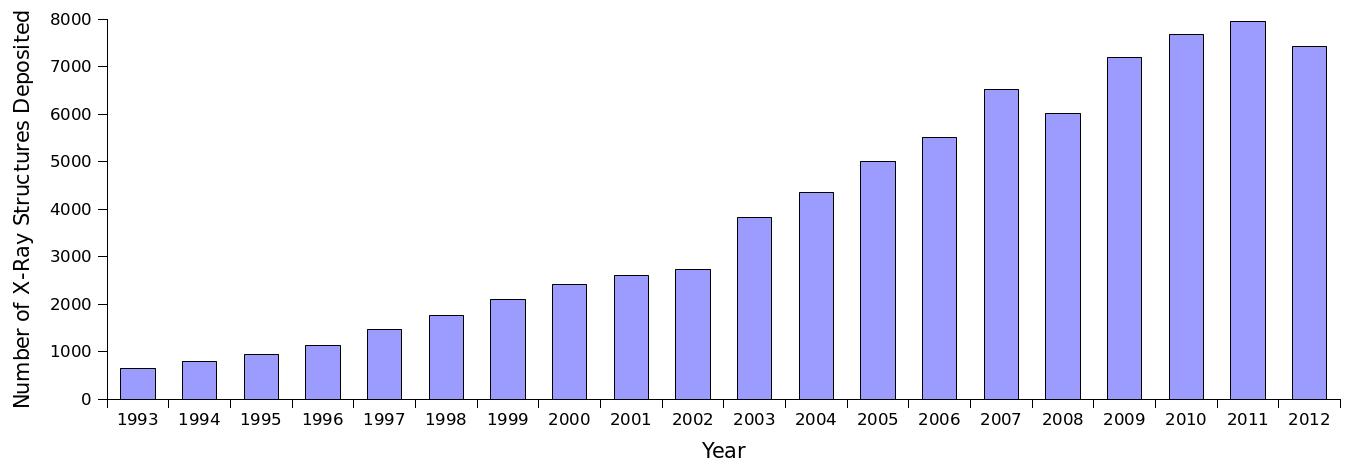
\includegraphics[width=\textwidth]{figures/pdb_deposit_rate.png}
\caption{The rate at which new structures is deposited into the PDB over the last two decades.
Due to a variety of improvements in the field of crystallography this rate has been steadily increasing.}
\label{figure:pdb_growth}
\end{center}
\end{figure}

% expected future growth of pdb
For example a recent increase in the field of crystallography, is ``crystal-less'' crystallography in which small molecules are bound by a porous scaffold matrix.
The regular structure of the matrix imparts a regular packing arrangement, necessary for interpreting diffraction patterns, onto the arrangement of small molecules.
This has the potential to address one of the largest difficulties in obtaining quality structural data for proteins, which is that it is very difficult to purify and crystallize certain proteins \cite{inokuma2013x}.

% unsorted
The number of target molecules of the set of all drugs currently available on the market consists of only about 500 proteins.
The bottleneck in introduction of new chemical entities is not virtual screening, but rather optimizing these hits into higher affinity leads and eventually balancing the requirements across all characteristics to produce a new drug \cite{bleicher2003hit}.

% unsorted
Of the total proteome only ~30,000 are regulated by small molecule binding, making them reasonable targets of drug action.
A large number of these possible drug targets are not implicated in any disease, due to this and a number of other factors, estimates of the total number of these proteins which are possible drug targets is much lower.
Frequently cited numbers for the number of possible drug targets in humans are six-hundred to fifteen-hundred, still significantly higher than the total number of targets which are exploited by current drugs.
The different families of cellular proteins are not equally likely to be targets of drugs.
As of {\the\year} 47\% of current drug targets are enzymes, followed by 30\% being GPCR's \cite{hopkins2002druggable}.

% drug-likeness
The consists of a number of characteristics which are generally true of drug like molecules:
\begin{enumerate}
\item Five or fewer hydrogen bond donors,
\item 500 Da or less total molecular mass
\item high liphophilicity
\item sum of nitrogen and oxygen atoms is not greater than 10 \cite{rule_of_five}
\end{enumerate}

% unedited
Through understanding the protein-ligand conformation and specific contacts they were able to modify a known substrate 
There is an advantage to flexible substrates, which is that they can flex in order to create better contacts with the protein structure increasing binding affinity.
This is especially important as the location of heavy atoms in the target protein is frequently only known to an accuracy of ~0.4 angstroms.
Further specific knowledge of the binding geometry between the initial lead compound and the target makes it possible to computationally screen possible chemical group substituents, to maximize binding affinity, increase solubility or bioavailability.
One of the earliest examples of the successful application of structure based drug design is the carbonic anhydrase inhibitor dorzolamide, in which most of these ideas were applied to find a drug with very high binding affinity \cite{greer1994application}.

% limitations
Despite advantages in speed and cost due to limitations in accuracy computational screening has struggled to produce the same results as empirical screening.
However, more recently virtual screening has succeeded in producing hit rates greater than those from empirical screening techniques.
Virtual screening has been used to identified leads which were later developed into the human immunodeficiency virus (HIV) protease inhibitor Viracept, and the anti-influenza drug Relenza.
\begin{figure}[h]
    \centering
    \begin{subfigure}[b]{0.3\textwidth}
        \centering
        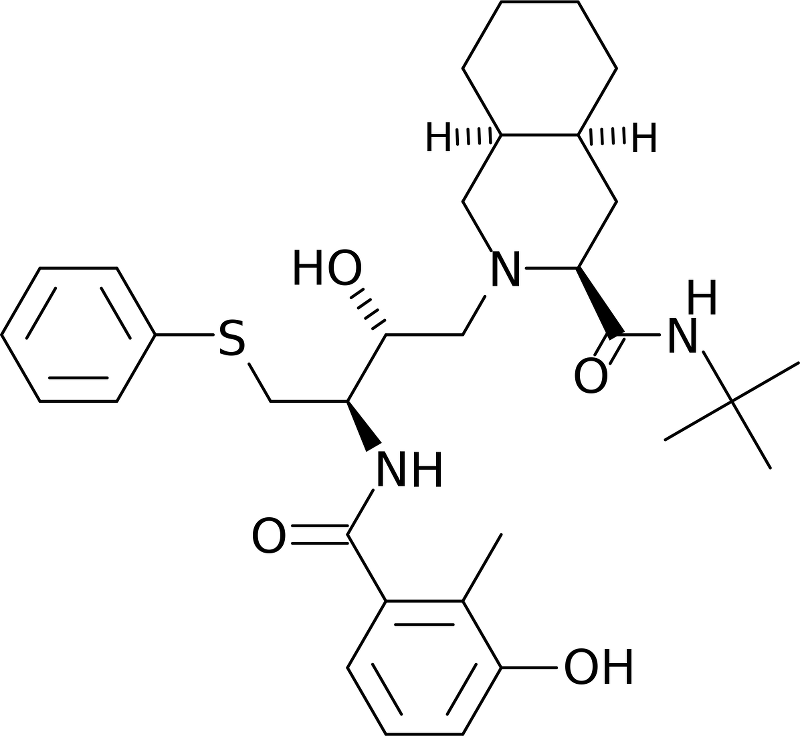
\includegraphics[width=\textwidth]{figures/nelfinavir_small.png}
        \label{fig:nelfinavir_chemical}
        \caption{}
    \end{subfigure}%
    \hspace{0.1\textwidth}
    \begin{subfigure}[b]{0.3\textwidth}
        \centering
        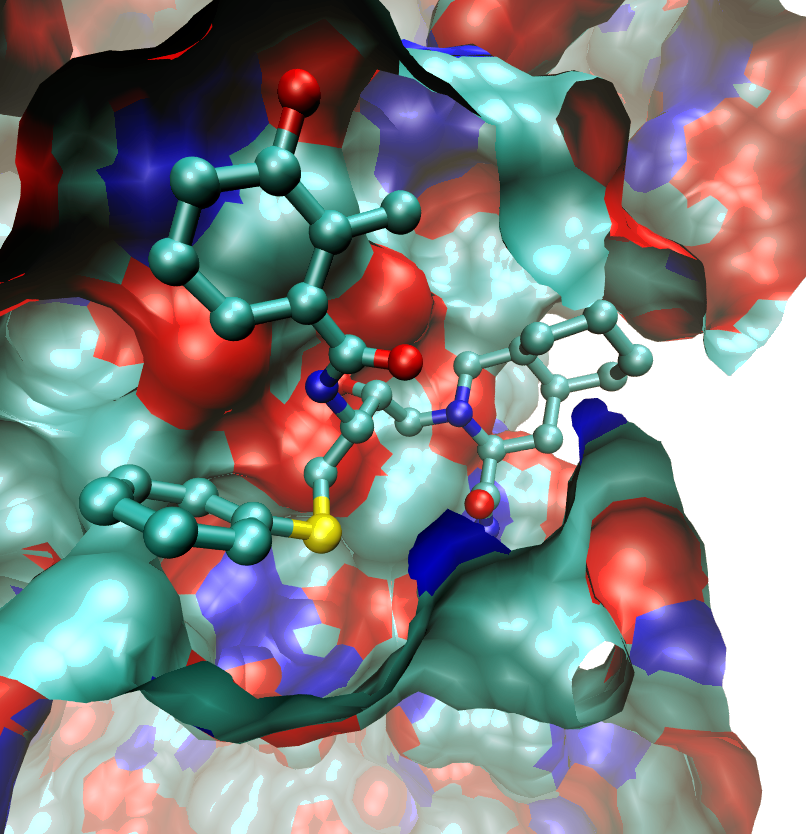
\includegraphics[width=\textwidth]{figures/complexed_nelfinavir_white.png}
        \label{fig:nelfinavir_docked}
        \caption{}
    \end{subfigure}
    \label{fig:nelfinavir}
    \caption{
The HIV protease inhibitor, nelfinavir, marketed under the name Viracept was originally identified using a computational docking screen.
It has a very high binding affinity for its target protein, 2 nM.
Here it is shown crystallized with multidrug variant (ACT) (V82T/I84V) of HIV-1 protease, PDBID 3EL5.
(b) generated with Visual Molecular Dynamics \protect\cite{humphrey1996vmd} and \protect\cite{povray}.
}
\end{figure}
A number of challenges which limit the utility of docking programs have been identified
\begin{enumerate}
\item The number of possible small molecules is essentially unbounded, however only a very small fraction of these ligands are potentially drug compounds. Limiting sampling to this subspace is a challenging problem.
\item The number of conformations of ligand molecules rises exponentially with the number of internal degrees of freedom of the ligand. Sampling the huge conformational space of the ligand becomes a computationally difficult problem on its own.
\item The difficulty of accurately assessing or comparing the energy of different protein-ligand complexes or conformations\cite{shoichet2004virtual}.
\end{enumerate}

% similarity between hits and leads
It has been found that introduced drugs are often very chemically similar the ``hit'' compounds from which they were derived \cite{proudfoot2002drugs}.
So in order to increase the diversity of drugs and find drugs which are able to treat new diseases, or diseases which have evolved resistance to current drugs it may be necessary to either increase the size of the screened database or increase the possible diversity which might be increase through the hit-to-lead step.

%\cite{kitchen2004docking}

\subsubsection{Hit-to-Lead Optimization}
\label{subsubsection:hit_to_lead}
Hit compounds generally have a binding affinity for the target protein on the order of micromolar binding.
The goals of hit-to-lead optimization are to further increase that affinity with the goal of eventually reaching binding affinities on the order of ~10 nanomolar or better, find other molecules with similar chemical characteristics to increase the size and diversity of the set of lead compounds, and screening hit compounds for any obvious issues.
At this stage for computational screening more accurate energy models are required than for the initial screen \cite{jorgensen2004many,gohlke2002approaches,jorgensen2009efficient}.
Depending on the type of ``hit'' compounds identified in the initial screen, hits are either combined through molecular-growing and evolution techniques, or similar structures to the hit compounds can be sampled either by exploring the local chemical space or ``mutation'' of substituents.
In either case, the potential lead compound is docked or grown in the known binding site.
A scoring function which is hopefully well correlated with the binding energy is then used to rank these possible compounds.
Interestingly it is not necessarily the case that the scoring function is anchored in a physical force field, it is possible to use statistical or artificial intelligence approaches with success, so long as they are able to successfully solve the classification problem of distinguishing strong binders from weak binders.
Docking as a means of converting hit compounds to lead compounds is very similar to docking as a means of hit generation, however in this case the small molecule library is much smaller and is generated to cover chemical space surrounding hit compounds.
Additionally whereas for initial hit generation a coarse grained energy function might have been sufficient to differentiate ligands which bind strongly from those which do not bind at all, to convert these ``hits'' to lead compounds it is necessary to use a more sensitive, and necessarily slower, energy model to accurately rank the binding affinity of different small molecules \cite{jorgensen2004many,gohlke2002approaches}.
These energy models will be discussed briefly in \ref{subsection:energy_functions}.

A popular program for building, or mutating lead compounds is Biochemical and Organic Model Builder (BOMB) \cite{barreiro2007docking}.
BOMB can operated as either a hit identification program or as a hit to lead optimization method.
Working to identify new compounds BOMB starts with a number of different small ``core'' scaffolds and attempts to increase binding affinity by adding or replace substituents with favorable interactions while avoiding steric clashes.
BOMB has been successfully used to evolve a hit compound which showed no inhibition of HIV reverse transcriptase into a potent non-nucleoside RT inhibitor with nanomolar level binding \cite{barreiro2007docking}.

Whereas previously, lead compounds were evaluated almost exclusively on binding affinity to the target protein, more recently more weight is being placed on identifying hit compounds which satisfy other characterisitcs besides binding affinity \cite{bleicher2003hit}.
It is important to begin to consider other characterisitcs of the potential drugs earlier in the pre-clinical process, because later it is difficult to make changes which affect characterisitcs such as solubility without significantly altering the binding affinity of an already highly modified hit compound.
As ``lead'' compounds are rarely very chemically distinct from the hits from which they were derived, and increasing binding affinity is actually sometimes an easier problem than addressing some of the other characteristics in the ``rule of five'' it is reasonable to begin by first trying to optimize hit compounds to satisfy some other criteria and postpone maximizing binding affinity \cite{proudfoot2002drugs}.

\subsubsection{Lead Optimization}
\label{subsubsection:lead_optimization}
In lead optimization the compounds which have been identified by the earlier steps in the process are optimized to drug molecules.
The largest differentiating factor between hit-to-lead optimization and lead optimization is the plausibility of the compound to act as a successful drug molecule.
The goals of lead optimization overlap heavily with those of the hit-to-lead stage.
Although this can include increasing binding affinity to the target even further, usually the focus is on other characteristics including selectivity, ease of synthesis, pharmacokinetic properties and intellectual property concerns \cite{keserHu2006hit}.
Computational modelling can help not only identify hit compounds, and convert those initial hits into leads, but also to help estimate absorption, distribution, metabolism, elimination, toxicology, sometimes referred to as the ADME characteristics \cite{kerns2008drug}.

Computational models for ADME characteristics ususally use regression equations or neural networks to predict these characteristics \cite{jorgensen2004many}.

Up to one half of all drugs which do not survive clinical trials, fail to do so because of lack of efficacy, which is influenced both by binding, but also by the absorption characteristics of the molecule.
The number of drugs which fail to make it through clinical trials due to toxcicity is similarly high, about 40\% \cite{li2001screening}.
Advancing a potential drug to clinical trials represents a very large financial investment, and effective computational screens of lead molecules at this point in the process can reduce the rate of failure in clinical trials, thereby having a very large impact on the final costs of new drugs brought to market.



\subsection{Computer Assisted Drug Design}
\label{subsection:computer_assisted_drug_design}
The ultimate goal of computer assisted drug design is to improve rational drug design by exploiting the continuously increasing processing power available both in high performance super computers, but also in single workstations.
Seeking to supplement the ability of a researcher either by allowing examination of a large number of possible interactions quickly or providing some insight that might be much more difficult to obtain through biochemical experiments, both in terms of time and expense.
Different classes of programs have been developed to help solve each of the distinct steps in the pre-clinical stages of drug development, namely:
\begin{enumerate}
\item Hit Identification – the process of screening a large small molecule database (up to one million or more small molecules) database to identify small molecules which bind a given target protein, or hits.
These hits are usually small molecules with a target binding affinity on the order of micromolar.
\item Hit to lead optimization - the process of modifying these ``hit'' molecules either by substitution or addition of chemical moieties or mixing and matching substructures between given hits, to produce compounds with higher binding affinities than the initial hit compounds.
Hit to lead optimization seeks to improve the micromolar binding affinity of hit compounds to nanomolar affinity or better.
\item Lead Optimization – the final step of modifying lead compounds to increase ``druglikeness'' to ensure that the molecule is sufficiently soluble, well tolerated, and does not disrupt regular cellular function.
\end{enumerate}

\subsubsection{Hit Identification}
\label{subsubsection:hit_identification}
% hit identification in general
The earliest form of hit identification experiments were animal screens, where mutant animals were studied to find the specific gene or protein causing a specific phenotype.
This type of experiment relies on careful genetic controls and breeding, but also some element of luck in observing a relevant phenotype in the first place.
``Brute force'' animal screens have since been improved with extensive mutation libraries and exhaustive non-lethal mutation libraries for organisms such as yeast and {\it Escherichia coli}.
Even so, these screens are slow, often taking three years or longer, and error prone, as performing a large number of repetitive experiments causes even the most fastidious of scientists to lose focus.
High-throughput screening seeks to supplement the human factor with robots, which are capable of performing similar experiments with greater speed and fewer errors.
With the help of this automation it is possible to test the interactions of as many as 100 million different reactions per day \cite{agresti2010ultrahigh}.
Though the high initial cost of high-throughput screening equipment as well as the cost of the small molecule libraries necessary for screening are often prohibitive even to large research institutions.
In order to make this sort of experiment available to a larger number of institutions some research institutions have instituted means of sharing this equipment, through high-throughput screening as a service type arrangements \cite{htsrc,mssr}.

% computational equivalents of hit identification
The direct computational equivalent to high-throughput screening is virtual screening, where a library of small molecules is computational ``docked'' into the active site of the target protein, and some scoring metric is used to identify possible binders.
In this sort of computational screen, he problem of the cost of small molecule libraries is essentially a solved problem in virtual screening as there are readily available libraries of drug-like small molecules for use in virtual screening programs.
For example, the ZINC database provides a library of over seven-hundred thousand commercially available small molecules in a number of different file formats for use in virtual screening \cite{irwin2005zinc}.
Another possibility for hit identification {\it in silico} is through fragment assembly methods.

% early docking history
The first published study using computational docking was published in 1982 by Irwin Kuntz describing a program which would later go on to become the well known DOCK program \cite{kuntz1982geometric}.
Generally docking consists of a method of quickly screening possible protein-small-molecule interaction conformations.
An emphasis is placed on the computational cost of evaluating the energy function over accuracy, as the poses generated by this step are usually fed into structural refinement programs for further sampling and more accurate estimation of energies.
For example in the original Kuntz study, the system only only had six degrees of freedom on which to sample, three translational and three rotational degrees of freedom for the ligand with the protein held fixed.
Along with a hard sphere collision model this provided a sufficiently selective screen to identify the native binding geometry of the heme group to myoglobin as well as thyroid hormone analogs to prealbumin \cite{kuntz1982geometric}.

% growth of pdb data
The rate at which new structures are being deposited into the Protein Data Bank is increasing on an annual basis.
But tools are necessary to draw meaningful insights from this data, hopefully leading to new drugs.
\begin{figure}[H]
\begin{center}
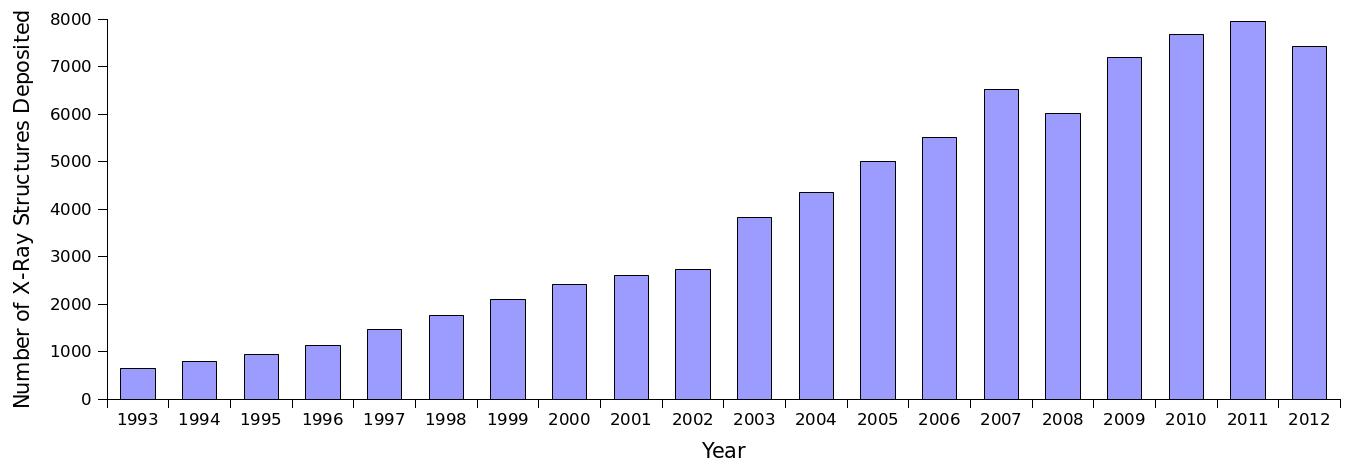
\includegraphics[width=\textwidth]{figures/pdb_deposit_rate.png}
\caption{The rate at which new structures is deposited into the PDB over the last two decades.
Due to a variety of improvements in the field of crystallography this rate has been steadily increasing.}
\label{figure:pdb_growth}
\end{center}
\end{figure}

% expected future growth of pdb
For example a recent increase in the field of crystallography, is ``crystal-less'' crystallography in which small molecules are bound by a porous scaffold matrix.
The regular structure of the matrix imparts a regular packing arrangement, necessary for interpreting diffraction patterns, onto the arrangement of small molecules.
This has the potential to address one of the largest difficulties in obtaining quality structural data for proteins, which is that it is very difficult to purify and crystallize certain proteins \cite{inokuma2013x}.

% unsorted
The number of target molecules of the set of all drugs currently available on the market consists of only about 500 proteins.
The bottleneck in introduction of new chemical entities is not virtual screening, but rather optimizing these hits into higher affinity leads and eventually balancing the requirements across all characteristics to produce a new drug \cite{bleicher2003hit}.

% unsorted
Of the total proteome only ~30,000 are regulated by small molecule binding, making them reasonable targets of drug action.
A large number of these possible drug targets are not implicated in any disease, due to this and a number of other factors, estimates of the total number of these proteins which are possible drug targets is much lower.
Frequently cited numbers for the number of possible drug targets in humans are six-hundred to fifteen-hundred, still significantly higher than the total number of targets which are exploited by current drugs.
The different families of cellular proteins are not equally likely to be targets of drugs.
As of {\the\year} 47\% of current drug targets are enzymes, followed by 30\% being GPCR's \cite{hopkins2002druggable}.

% drug-likeness
The consists of a number of characteristics which are generally true of drug like molecules:
\begin{enumerate}
\item Five or fewer hydrogen bond donors,
\item 500 Da or less total molecular mass
\item high liphophilicity
\item sum of nitrogen and oxygen atoms is not greater than 10 \cite{rule_of_five}
\end{enumerate}

% unedited
Through understanding the protein-ligand conformation and specific contacts they were able to modify a known substrate 
There is an advantage to flexible substrates, which is that they can flex in order to create better contacts with the protein structure increasing binding affinity.
This is especially important as the location of heavy atoms in the target protein is frequently only known to an accuracy of ~0.4 angstroms.
Further specific knowledge of the binding geometry between the initial lead compound and the target makes it possible to computationally screen possible chemical group substituents, to maximize binding affinity, increase solubility or bioavailability.
One of the earliest examples of the successful application of structure based drug design is the carbonic anhydrase inhibitor dorzolamide, in which most of these ideas were applied to find a drug with very high binding affinity \cite{greer1994application}.

% limitations
Despite advantages in speed and cost due to limitations in accuracy computational screening has struggled to produce the same results as empirical screening.
However, more recently virtual screening has succeeded in producing hit rates greater than those from empirical screening techniques.
Virtual screening has been used to identified leads which were later developed into the human immunodeficiency virus (HIV) protease inhibitor Viracept, and the anti-influenza drug Relenza.
\begin{figure}[h]
    \centering
    \begin{subfigure}[b]{0.3\textwidth}
        \centering
        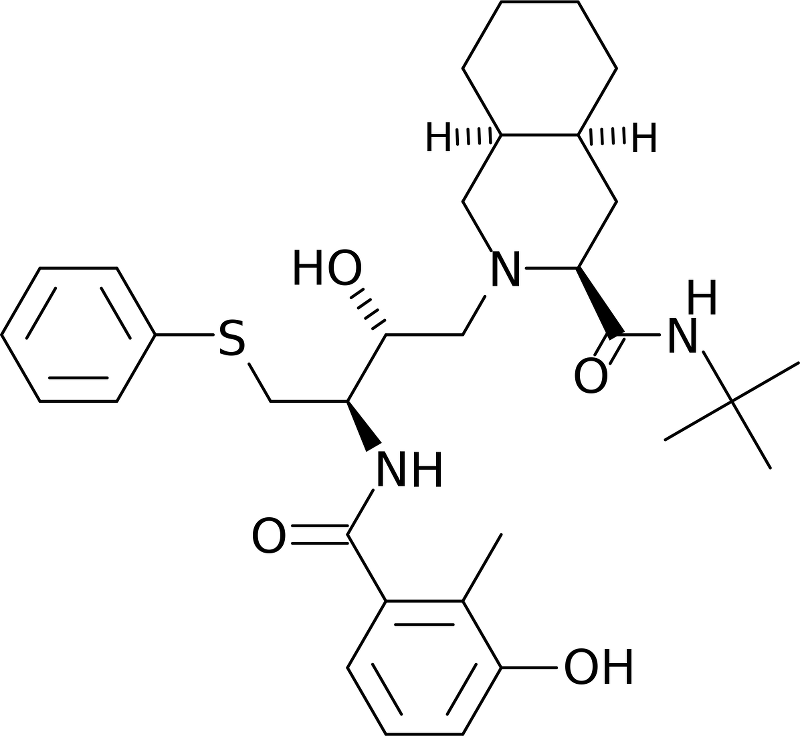
\includegraphics[width=\textwidth]{figures/nelfinavir_small.png}
        \label{fig:nelfinavir_chemical}
        \caption{}
    \end{subfigure}%
    \hspace{0.1\textwidth}
    \begin{subfigure}[b]{0.3\textwidth}
        \centering
        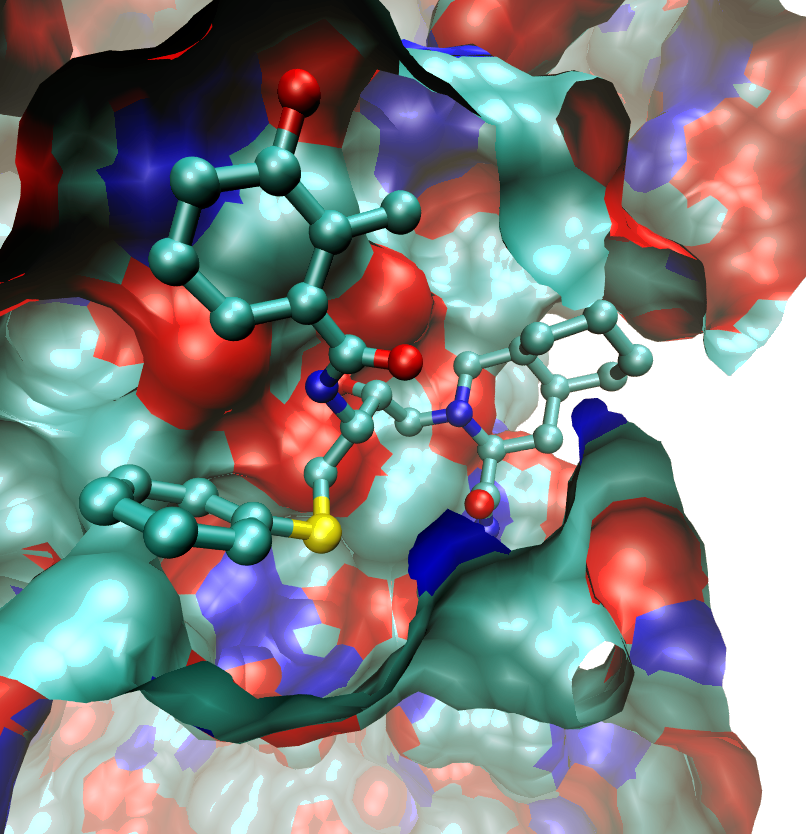
\includegraphics[width=\textwidth]{figures/complexed_nelfinavir_white.png}
        \label{fig:nelfinavir_docked}
        \caption{}
    \end{subfigure}
    \label{fig:nelfinavir}
    \caption{
The HIV protease inhibitor, nelfinavir, marketed under the name Viracept was originally identified using a computational docking screen.
It has a very high binding affinity for its target protein, 2 nM.
Here it is shown crystallized with multidrug variant (ACT) (V82T/I84V) of HIV-1 protease, PDBID 3EL5.
(b) generated with Visual Molecular Dynamics \protect\cite{humphrey1996vmd} and \protect\cite{povray}.
}
\end{figure}
A number of challenges which limit the utility of docking programs have been identified
\begin{enumerate}
\item The number of possible small molecules is essentially unbounded, however only a very small fraction of these ligands are potentially drug compounds. Limiting sampling to this subspace is a challenging problem.
\item The number of conformations of ligand molecules rises exponentially with the number of internal degrees of freedom of the ligand. Sampling the huge conformational space of the ligand becomes a computationally difficult problem on its own.
\item The difficulty of accurately assessing or comparing the energy of different protein-ligand complexes or conformations\cite{shoichet2004virtual}.
\end{enumerate}

% similarity between hits and leads
It has been found that introduced drugs are often very chemically similar the ``hit'' compounds from which they were derived \cite{proudfoot2002drugs}.
So in order to increase the diversity of drugs and find drugs which are able to treat new diseases, or diseases which have evolved resistance to current drugs it may be necessary to either increase the size of the screened database or increase the possible diversity which might be increase through the hit-to-lead step.

%\cite{kitchen2004docking}

\subsubsection{Hit-to-Lead Optimization}
\label{subsubsection:hit_to_lead}
Hit compounds generally have a binding affinity for the target protein on the order of micromolar binding.
The goals of hit-to-lead optimization are to further increase that affinity with the goal of eventually reaching binding affinities on the order of ~10 nanomolar or better, find other molecules with similar chemical characteristics to increase the size and diversity of the set of lead compounds, and screening hit compounds for any obvious issues.
At this stage for computational screening more accurate energy models are required than for the initial screen \cite{jorgensen2004many,gohlke2002approaches,jorgensen2009efficient}.
Depending on the type of ``hit'' compounds identified in the initial screen, hits are either combined through molecular-growing and evolution techniques, or similar structures to the hit compounds can be sampled either by exploring the local chemical space or ``mutation'' of substituents.
In either case, the potential lead compound is docked or grown in the known binding site.
A scoring function which is hopefully well correlated with the binding energy is then used to rank these possible compounds.
Interestingly it is not necessarily the case that the scoring function is anchored in a physical force field, it is possible to use statistical or artificial intelligence approaches with success, so long as they are able to successfully solve the classification problem of distinguishing strong binders from weak binders.
Docking as a means of converting hit compounds to lead compounds is very similar to docking as a means of hit generation, however in this case the small molecule library is much smaller and is generated to cover chemical space surrounding hit compounds.
Additionally whereas for initial hit generation a coarse grained energy function might have been sufficient to differentiate ligands which bind strongly from those which do not bind at all, to convert these ``hits'' to lead compounds it is necessary to use a more sensitive, and necessarily slower, energy model to accurately rank the binding affinity of different small molecules \cite{jorgensen2004many,gohlke2002approaches}.
These energy models will be discussed briefly in \ref{subsection:energy_functions}.

A popular program for building, or mutating lead compounds is Biochemical and Organic Model Builder (BOMB) \cite{barreiro2007docking}.
BOMB can operated as either a hit identification program or as a hit to lead optimization method.
Working to identify new compounds BOMB starts with a number of different small ``core'' scaffolds and attempts to increase binding affinity by adding or replace substituents with favorable interactions while avoiding steric clashes.
BOMB has been successfully used to evolve a hit compound which showed no inhibition of HIV reverse transcriptase into a potent non-nucleoside RT inhibitor with nanomolar level binding \cite{barreiro2007docking}.

Whereas previously, lead compounds were evaluated almost exclusively on binding affinity to the target protein, more recently more weight is being placed on identifying hit compounds which satisfy other characterisitcs besides binding affinity \cite{bleicher2003hit}.
It is important to begin to consider other characterisitcs of the potential drugs earlier in the pre-clinical process, because later it is difficult to make changes which affect characterisitcs such as solubility without significantly altering the binding affinity of an already highly modified hit compound.
As ``lead'' compounds are rarely very chemically distinct from the hits from which they were derived, and increasing binding affinity is actually sometimes an easier problem than addressing some of the other characteristics in the ``rule of five'' it is reasonable to begin by first trying to optimize hit compounds to satisfy some other criteria and postpone maximizing binding affinity \cite{proudfoot2002drugs}.

\subsubsection{Lead Optimization}
\label{subsubsection:lead_optimization}
In lead optimization the compounds which have been identified by the earlier steps in the process are optimized to drug molecules.
The largest differentiating factor between hit-to-lead optimization and lead optimization is the plausibility of the compound to act as a successful drug molecule.
The goals of lead optimization overlap heavily with those of the hit-to-lead stage.
Although this can include increasing binding affinity to the target even further, usually the focus is on other characteristics including selectivity, ease of synthesis, pharmacokinetic properties and intellectual property concerns \cite{keserHu2006hit}.
Computational modelling can help not only identify hit compounds, and convert those initial hits into leads, but also to help estimate absorption, distribution, metabolism, elimination, toxicology, sometimes referred to as the ADME characteristics \cite{kerns2008drug}.

Computational models for ADME characteristics ususally use regression equations or neural networks to predict these characteristics \cite{jorgensen2004many}.

Up to one half of all drugs which do not survive clinical trials, fail to do so because of lack of efficacy, which is influenced both by binding, but also by the absorption characteristics of the molecule.
The number of drugs which fail to make it through clinical trials due to toxcicity is similarly high, about 40\% \cite{li2001screening}.
Advancing a potential drug to clinical trials represents a very large financial investment, and effective computational screens of lead molecules at this point in the process can reduce the rate of failure in clinical trials, thereby having a very large impact on the final costs of new drugs brought to market.


\section{Molecular Modeling}
\label{section:molecular_modeling}
Molecular modeling seeks to gain new insights into the real world behavior of molecules by mimicking these molecules, usually using computer simulations.
According to the theory of ``minimal frustration'' the protein native state is not only a low energy state, but is also stable \cite{bryngelson1987spin}.
So the prediction of native or native-like conformations focuses on finding those conformations which have a low potential energy.
As measuring the true potential energy of a system is very difficult or impossible computational models seek to reproduce the qualitative behavior of the energy surface.
Quantum mechanics calculations are often viewed as the gold standard with respect to intramolecular energy calculations.
However, despite the accuracy of quantum mechanics, its application to large systems such as proteins is currently limited due to the amount of time necessary to perform quantum mechanics calculations on a large number of atoms.
Instead quantum mechanics calculations have been used to parameterize a majority of the most popular molecular mechanics force fields currently in use, including:
\begin{enumerate}
\item AMBER \cite{weiner1984new},
\item OPLS-AA \cite{kaminski1994free},
\item and CHARMM \cite{mackerell2002charmm}.
\end{enumerate}

The earliest molecular mechanics force fields either modeled groups of atoms as a unit, hydrogens being grouped with their bound heavy atom \cite{jorgensen1988opls}, or even each residue as a unit \cite{lee1999energy}, both to reduce the number of parameters in the model and to increase the speed of computations.
Although {\it ab initio} folding experiments are theoretically interesting, they are generally not practical both because of the difficulty in simulating such a large system for the time-frame necessary to observe behaviors like folding, and also because structural models for many proteins are available either directly as X-ray structures, or indirectly through homology.

\begin{figure}[h]
\begin{center}
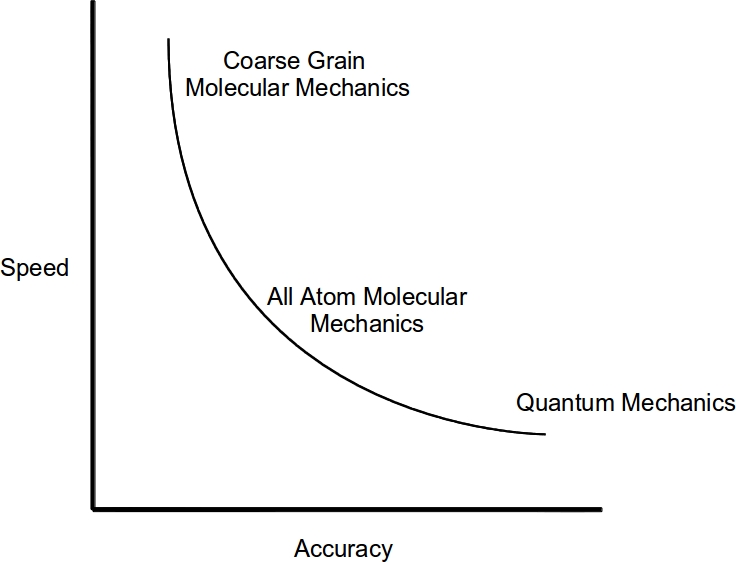
\includegraphics[width=0.7\textwidth]{figures/conservation_of_annoyance.png}
\caption{To an extent it is always possible to either increase accuracy or decrease running time, or the cost of an experiment.
New scientific methods should allow one to increase accuracy while not spending additional time.}
\label{figure:conservation_of_annoyance}
\end{center}
\end{figure}

Because of the evolutionary cost of mis-folded proteins, proteins have been selected to minimize mis-folding, making the general shape of the potential energy surface roughly funnel shaped with the native structure at the minimum \cite{leopold1992protein}.
Despite this shape, the energy landscape of proteins is a very ``jagged'' surface with a large number of local minima \cite{tsai1999folding}.

Even the smallest enzyme contains 62 amino acids, and has thousands of degrees of freedom \cite{chen19924}, and larger enzymes are regularly more than 1000 amino acids.
The number of degrees of freedom of these systems make any attempt to analytically solve for a global minimum energy conformation impossible, and require other methods of generating plausible conformations.
In order to compensate for this a number of different sampling methods have been developed.

%\subsection{Sampling Methods}
%\label{subsection:sampling_methods}

%    \subsubsection{Minimization}
%    \label{subsubsection:minimization}
%    Minimization techniques seek to find the lowest energy conformation in a given potential well.
Generally, they make no attempt to sample outside of that well, and therefore are frequently implemented as a final stage in sampling, in order to relieve any unfavorable interactions in proposed structures.
There are a large number of different minimization techniques, and they will not be covered in any real depth here, please see the original papers for more details, or \cite{schlick2010molecular} for a review.
As the basic terms of the general molecular mechanics potential energy function are differentiable, and discounting for the moment the significant effects of solvent, it is possible to solve for the energy gradient, or force on every atom for a given conformation.
A few minimizations methods include:
\begin{enumerate}
\item ``Steepest descent'', conceptually the simplest minimization algorithm, in which the gradient is calculated at each step, and the size of the step is proportional to the magnitude of the gradient \cite{levitt1969refinement,bixon1967potential}.
\item ``Newton'' methods instead of approximating the gradient as a linear function in a small neighborhood, express the gradient, as a quadratic function.  This has been shown to converge more quickly than steepest descent \cite{ponder1987efficient}.  
Discrete Newton and Quasi-Newton methods use numeric estimation techniques instead of analytically solving for the gradient \cite{schlick2010molecular}.
\item ``Truncated Newton'' methods find an approximate solution to Newton's equations, forcing the residual to approach zero as the series converges \cite{dembo1983truncated}. 
\end{enumerate}

% molecular mechanics burkert allinger

%Quasi-Newton methods like ABNR of CHARMM estimate the hessian, instead of computing it directly, by accumulating residuals over multiple steps \cite{chu2003super}.


%    \subsubsection{Monte-Carlo Sampling}
%    \label{subsubsection:monte_carlo}
%    Metropolis Monte-Carlo simulation was originally developed in the 1950's to provide rapid sampling of the solution space of many variable problems \cite{metropolis1953equation,hastings1970monte}.
Monte-Carlo techniques generate a sequence of states from a distribution by proposing a new state based only on the current state 
If the ensemble average is the same as the sequence average, a Monte Carlo Markov chain can be used to estimate ensemble averages, this is known as {\it ergodicicy} \cite{schlick2010molecular}.
Another requirement is {\it detailed balance} that the probability of transition from a state $X_{i}$ to a state $X_{i+1}$ is the same as the probability of the reverse transition, i.e. $X_{i+1}$ to $X_{i}$.
By setting the probability of acceptance to
\input{equations/metropolis_acceptance}
these conditions are met.

In molecular mechanics, Metropolis Monte Carlo provides a very efficient means of sampling conformation space and a simple method of estimating the distribution of states.
Modifications on this method, such as annealing, where the temperature is continuously decreased over the course of the simulation, or umbrella sampling, which attempts to achieve better sampling in cases where a potential energy barrier divides two or more states from each other \cite{torrie1977nonphysical}.
While Monte Carlo sampling techniques are very fast to provide new states, the majority of these states reflect higher energy conformations.
Since it is of practical biological interest, Monte Carlo minimization has been developed to increase the rate at which minima are sampled \cite{li1987monte}.



%    \subsubsection{Analytic Loop Closure}
%    \label{subsubsection:analytic_loop_closure}
%    Subsequences with regular secondary structures, i.e. $\alpha$-helices and $\beta$-sheets are generally better conserved, and therefore likely to be well covered by simple homology models \cite{kolodny2005inverse,petrey2003using}.
The intervening ``random coil'' or loop regions often play a large role in determining protein specificity for a specific ligand, as in antigen-antibody binding \cite{bajorath1996comparison}, small protein toxins to the receptors they target \cite{wu1996functional}, or transcription factors to specific DNA sequences \cite{jones1999protein}.

Loop closure or prediction is a significant part of homology modeling \cite{petrey2003using} and building structures consistent with X-ray refraction data.
Therefore, in order to accurately predict three dimensional structure through homology models, infer protein binding partners and function, or even build a three dimensional structure consistent with both X-ray data and physical constraints, accurately predicting these loop regions is critical \cite{fiser2000modeling}.

The loop closure question is, given two fixed endpoints and a flexible loop, or actuator, how does one find a loop conformation, or set of conformations, that connects the two endpoints.
Because similar problems are frequently encountered in the field of robotics, a number of loop closure algorithms have been adapted from robotics \cite{kolodny2005inverse}.
The first of these algorithms is analytical loop closure, where a conformation that satisfies the closure criteria is solved for directly by solving a system of equations.
Though this problem can be solved analytically for small loops \cite{wedemeyer1999exact,go1970ring,bruccoleri1985chain,palmer1991standard}, the difficulty of the problem increases as loop length grows and the number of degrees of freedom of the loop section increases.
Additionally, these closure constraints make sampling multiple different conformations more difficult \cite{cortes2005sampling}, though it is possible to hierarchically solve sub-loops in order to generate conformations for possible complete loop conformations \cite{wedemeyer1999exact}.


%    \subsubsection{Random Tweak}
%    \label{subsubsection:tweak}
%    Random tweak, like CCD, is a method of producing and sampling closed loop conformations.
It begins in much the same way as CCD, by randomizing $\phi$ and $\psi$ dihedral angles of the loop backbone.
Random tweak seeks to close the loop while retaining dihedral angles as close to the randomized starting structure as possible.
By adjusting each dihedral only a small amount at a time and staying in the region where $sin(\theta) \approx \theta$, it is possible to formulate a set of linear equations to solve for a set of $\Delta\theta_{i}$, which minimizes the distance between the crystal position of the atom to be closed and the random position.
Because the assumption $sin(\theta) \approx \theta$ only holds for small $\theta$, the maximum change in angle is limited to 10 degrees in the original implementation of the random tweak algorithm.
Because almost all structures predicted using the random tweak or cyclic coordinate descent produce closed loops, a much smaller fraction of time is spent sampling loops that do not satisfy the closure criteria, making these algorithms very efficient \cite{fine1986predicting,shenkin1987predicting}.


%    \subsubsection{Cyclic Coordinate Descent}
%    \label{subsubsection:cyclic_coordinate_descent}
%    Another robotics algorithm which has been successfully applied to protein loop closure is Cyclic Coordinate Descent (CCD) \cite{canutescu2003cyclic}.
As the length of a flexible loop grows the number of degrees of freedom increases and the possible solution space grows exponentially. 
Cyclic coordinate descent seeks to close the loop by adjusting the degrees of freedom, in this case the $\phi$ and $\psi$ dihedral angles, sequentially and possibly iterating over each degree of freedom multiple times until the loop is closed.
This method is able to solve for conformations very quickly, and the likelyhood of closing a loop {\it increases} as the number of degrees of freedom of the system increases.

In cyclic coordinate descent the $\phi$ and $\psi$ angles of each loop backbone residue are first randomized.
Then a loop dihedral is chosen at random, and varied to move the last atom of the loop as near as possible to its desired position.
A new dihedral is chosen and optimized until the loop is closed.
It is possible that this procedure does not converge to a closed state, however experiments have shown that this is very unlikely even for extended loops with few degrees of freedom, $ < 2\%$ failure rate for 4 residue loops.
Solving for the ideal dihedral angle at each step is a simple optimization problem making CCD a very fast algorithm \cite{wang1991combined,canutescu2003cyclic}.
In experiments CCD produces closed loop candidates in ~1/6 the time of the random tweak method.

A variation on cyclic coordinate descent seeks to close the loop by not only requiring atom closure, but by requiring that the entire backbone of the closure residue is superimposed, within some geometric similarity tolerance, between the predicted and crystal structure.
This constrainint ensures that the angles and dihedrals of the closure residue are reasonable\cite{canutescu2003cyclic}.


%    \subsubsection{Rotamer Assembly}
%    \label{subsubsection:rotamer_assembly}
%    Rotamer assembly or systematic search shares some similarity with fragment buildup techniques in that it uses a rotamer library to assemble possible loops.
This rotamer library represents the common backbone dihedrals for each amino acid.
This method operates by dividing the loop into two pieces, usually in half, and considering all possible half loops which can be built using rotamer library \cite{moult1986algorithm}.
For each side of the loop a ``tree'' is considered in both a physical sense, that the hemi-loop branches as it grows away from its anchor, and a decision tree sense, in that every residue represents a decision where a single rotamer is selected from the rotamer library.
When the hemi-trees for each side of the gap are fully constructed some closure criteria is applied, in the case of the original systematic search geometric agreement is required of the entire mid-residue \cite{moult1986algorithm}, however a more lax criteria is applied in the case of the PLOP where only one atom is required to be approximately superimposed \cite{jacobson2004hierarchical}.
By carefully pruning trees during the building process, and biasing the search towards occupied regions of $\phi$-$\psi$ space, systematic search can be quite efficient, spending little time sampling implausible regions of conformation space.
Additionaly, by building residue pairs, using a smaller
 possibly restricting the rotamer library by building multiple residues at a time this sort of procedure has been used to build loops of 20+ residues \cite{zhao2011progress}.


% \cite{kolodny2005inverse}


\subsection{Energy Functions}
\label{subsection:energy_functions}
    \subsubsection{The General Form of the Energy Model}
    \label{subsubsection:energy_general_form}
    Some energy models do not seek to accurately rank potential conformations, fast ``screening'' functions attempt to quickly differentiate physically impossible conformations from plausible conformations without performing an expensive minimization or energy calculation step.
Application of these screening functions has the potential to greatly reduce the number of potential conformations that must be scored using the full detail energy function, greatly decreasing the overall cost of conformation prediction.
These screening criteria can be applied either during the sampling procedure, potentially eliminating sampling of a large area of excluded conformation space, or after sampling before a more expensive energy function is applied to rank conformations.
Effective screening criteria have a large impact on the total performance of a structure prediction method.

One of the earliest screening criteria was the hard sphere overlap collision detection \cite{levinthal1966molecular}, and this method is consistently included in screening scriteria.
Other screens include:
\begin{enumerate}
\item bounds on bond lengths and angles, as a single bond which deviates significantly from equilibrium can dominate the energy of a conformation,
\item limitations on $\phi$-$\psi$ space occuped by backbone dihedrals corresponding to the Ramachandran plot of the residue,
\item limiting side chain dihedrals to staggered conformations, which correspond to the low energy well of side chain dihedral space \cite{moult1986algorithm},
\item excluding structuctures which present excessive solvent accessible surface area, as this conflicts with the hydrophobic effect, which has a large effect on the conformation of the native state \cite{chothia1975principles}
\item limitations on the number of ``dry'' cavities, and the number of internal charged residues \cite{moult1986algorithm}
\end{enumerate}

The general form of most molecular mechanics energy potentials is reasonably consistent, with bonds and angles being modeled as a spring, dihedrals as a Fourier series.
\input{equations/opls.tex}
\input{equations/bonds.tex}
\input{equations/angles.tex}
\input{equations/dihedrals_compact.tex}
The non-bonded terms are modeled as a Columbic potential between any point charges and a Lennard-Jones or 6-12 potential between any non-bonded atoms.
These non-bonded atoms are phased in by a ``fudge factor'' for atoms in a 1-4 configuration.
\input{equations/nonbonded.tex}
Where $\sigma_{ij} = \sqrt{\sigma_{ii} \sigma_{jj}}$ and $\epsilon_{ij} = \sqrt{\epsilon_{ii}\epsilon_{jj}}$ \cite{jorgensen1996development}.



    \subsubsection{Molecular Surfaces}
    \label{subsubsection:molecular_surfaces}
    Central to the discussion of solvent is a discussion of how to formulate the surface of a protein.
The most frequently used formulations of surface area include:
\begin{enumerate}
\item The Van der Waals (VDW) surface is the surface formed by the VDW radius of each molecule, though sometimes differing parameters are used for the VDW radii, and the ideal radii may even vary by application.
\item The solvent accessible surface, which is defined as the surface traced by the center of a spherical probe ``rolled'' over the VDW surface \cite{richards1977areas}.  This idea is very closely related to the idea of the solvent excluded volume, or the shape of the solvent cavity enforced by the VDW surface of the molecule \cite{richmond1984solvent}.
\item The molecular surface, or Connolly surface, is composed of the VDW surface in areas where the spherical probe touches the VDW surface, in union with all points on the probe ``between'' two points on the VDW surface when the probe is contacting multiple atoms \cite{connolly1983analytical}, put another way the surface of the volume which intersects no possible probe location.
\end{enumerate}
Frequently these surfaces are approximated numerically, using the Shrake-Rupley algorithm \cite{shrake1973environment}, by considering a spherical mesh about every atom and including only points which satisfy the definition of the surface, or using these points to interpolate a surface.

The significance of surface area is determined by physical constraints but can be well illustrated by a number of observations about proteins.
First the ratio of total area of a theoretical unfolded, i.e. linearly arranged, protein to its length is almost among proteins, only varying by \textapprox 3\% between different proteins.


\subsection{Solvent Models}
\label{subsubsection:solvent_models}
The section on solvent models.




\chapter[Cell Based Implicit Solvent Model]{A Cell Based Method for Evaluating Implicit Solvation Effects}
\label{chapter:cell_solvent}

One can see in the Generalized Born model \eqref{equation:generalized_born}, computing the electrostatic contribution to solvation requires computing the distance between every two atoms.

\section{Introduction}
\label{section:cell/intro}
% super broad computational chemistry is important because
Computational protein structure prediction and related areas of research such as target screening and lead optimization continue to be areas of active research in both pure chemistry and pharmaceutical applications \cite{jorgensen2009efficient}.
These methods range from identifying leads using chemical similarity metrics, to artificial intelligence methods such as neural networks and support vector machines, to structural based methods \cite{geppert2010current}.
In the recent past, structural methods have contributed to the identification of bioactive drug compounds \cite{corsino2009novel}, making computational protein structure prediction highly important to the medical field, and because of its pharmaceutical applications, economically relevant as well.

% the expense of computational biology and necessity of fast algorithms 
There are over 81,000 X-ray structures presently in the PDB, more than 8,500 of which have been added in the last 12 months, and the rate at which new structures are determined by X-ray crystallography continues to accelerate (see figure \ref{figure:pdb_growth}) \cite{berman2007worldwide}.
The chemical space of small molecules, i.e. potential drug compounds, is essentially unlimited, and at the least too large to effectively screen using conventional experimental methods \cite{jorgensen2009efficient}. 
Furthermore, computational loop prediction experiments are predicting longer loops, increasingly relying on the output of initial predictions as the input to a later ``fixed stage'' refinement step that re-predicts some central region of the same loop.
This has been shown to increase accuracy \cite{jacobson2004hierarchical} at the cost of an increased number of experiments and corresponding increase in computational cost.
Taken together, these factors necessitate the development of more accurate and efficient methods of generating and evaluating protein-protein and protein-small molecule conformations and interactions.

% intro of plop and solvent models
The Protein Local Optimization Program (PLOP), originally developed by Friesner and co-workers, is a popular program used to predict, sample, and evaluate protein conformations \cite{jacobson2002role,jacobson2002force,jacobson2004hierarchical}.
PLOP makes use of the OPLS-AA energy model, an atomic detail force field optimized for organic, including protein, interactions \cite{jorgensen1996development}.
In addition to the terms defined by the OPLS-AA model, it has been shown that solvent effects can make a large contribution to prediction accuracy.
The solvent contribution to an energy model can be evaluated either by explicitly modeling and sampling solvent molecules (usually water) or by treating the solvent as a continuous medium, i.e. implicit solvation.
PLOP, like many other molecular mechanics programs, makes use of an implicit solvent model.
% introduction of explicit/implicit solvent
This is largely because explicitly modeling solvent molecules, while possibly very accurate, requires extensive, and therefore very time consuming, sampling of a large number of small molecules \cite{zhang2001solvent}.
Further, energy errors using explicit solvent models can be due to either unrealistic force field parameters or insufficient sampling of solvent molecule conformations \cite{zhou2003free}.
Continuum solvation methods, or implicit solvent methods, attempt to address these issues by removing the dependence on sampling of solvent molecules and introducing approximations that reduce the cost of calculating the solvent contribution to energy \cite{roux1999implicit}.

% talking about implicit solvent
Among implicit solvent methods, the surface area based generalized Born (S-GB) model is one of the most popular and has been shown to produce results in good agreement with experimental data \cite{zhang2001solvent,gallicchio2002sgb}.
The surface area based generalized Born implicit solvent model provides an approximate solution to the Poisson--Boltzmann equation based on a surface integral \cite{ghosh1998generalized}.
However, in a naive implementation of this model, the electrostatic contribution is a sum over every charge-charge pair in the system, in this case the protein and its crystal copies.
\begin{equation}
U = \sum_{charges}U_{self}(q_k,r_k) + \sum_{charges,\ i \ne j}U_{pair}(q_i,q_j,r_i,r_j)
\end{equation}

The electrostatic contribution to solvation free energy, can be decomposed into self, and pairwise terms.
The time complexity of evaluating the pair term is quadratic in the number of charges in the system \cite{ghosh1998generalized}.
This means that calculating the electrostatic solvation contribution for a single atom requires a linear search over all other charges in the system, which for large systems becomes the bottleneck of the computation.
A common optimization is to assume that the electrostatic contribution to the solvation term for point charges separated by a distance greater than a defined cutoff distance is negligible \cite{gallicchio2004agbnp}. 
However, making this assumption does not improve the underlying quadratic time complexity of evaluating the solvation term, as it is necessary to compute the inter-charge distance for every charge pair in the system before possibly excluding the interaction.
In the implementation of S-GB in the Protein Local Optimization Program, computing the solvation term of a large structure is the rate limiting step of energy calculations, accounting for over 80\% of the total time spent computing the energy (see figure \ref{fig:timing_pie}).
Therefore, less expensive methods of evaluating the implicit solvent contribution to the energy of a system can allow for increased sampling with the same available resources, thus improving efficiency of computational modeling. 

We present an application of a geometric hashing method, grid based spatial indexing, to implicit solvent calculations in PLOP.
The hashing method proceeds by dividing space into cubical regions, or cells, and distributing atoms into those cells, while maintaining a list of the contents of each.
Retrieval of atoms within a cell can then be performed in constant time, and retrieval of a superset of atoms contained within a region can be performed in time proportional to the number of cells intersecting the region.
This efficient geometric lookup allows one to replace a loop over all atoms inside the structure with a loop over only the atoms contained in cells intersecting the sphere with radius corresponding to the distance cutoff of the force in question.
While maintaining a list of atoms for each of these grid boxes introduces some overhead when updating atomic coordinates during a simulation, updating atomic coordinate is still a constant time operation.
Thus, the benefits outweigh the costs, especially for large systems.
As long as the cell size is bounded below, the number of cells necessary to consider when evaluating a fixed distance interaction is constant.
Physical limitations provide an upper limit to atom density.
Constant time retrieval of the contents of each hash cell, along with upper bounds on the number of atoms per cell and the necessary number of cells to consider for each charge, guarantee constant time lookup of all atoms within a given sphere.
This reduces the time complexity of evaluating the electrostatic contribution from $O(n^2)$ to $O(n)$.
We show that an implementation of this hashing method can reproduce results obtained with a non-hash based implementation while providing significant performance improvements.



\section{Methods}
\label{section:cell/methods}
    \subsection{Energy Model}
    \label{subsection:energy_model}
    The energy model used in side chain prediction experiments was the optimized variable dielectric model (OVD), sometimes referenced as the variable dielectric surface generalized Born 2.0 model (VSGB2.0).
This energy model is based on the OPLS-AA energy model, which in turn gets most of its covalent parameters from the AMBER force field \cite{jorgensen1996development}.
The solvation term used is a surface area based generalized Born formulation, where the internal dielectrics of charged amino acids have been optimized over a set of 2239 single side chain predictions and 100 loop predictions of 11 to 13 residue loops.
In addition to the covalent terms from the OPLS-AA model, the current energy model also includes terms to describe $\pi-\pi$ stacking, hydrogen bonding, and a parametrized hydrophobic term for the non-polar free energy of solvation \cite{li2011vsgb}.
For the electrostatic contribution to solvation free energy, two different molecular surfaces are maintained at different resolutions.
A surface mesh is constructed for each atom using the generalized spiral points method \cite{rakhmanov1994minimal,saff1997distributing,zhou1995arrangements}.
The number of points for each sphere is 10 for the low resolution surface and 330 for the high resolution surface.
An atomic based distance cutoff is used when evaluating the electrostatic contribution to the solvation free energy.
Inside a distance of $\sqrt{50}$ angstroms, the high resolution surface is used; between this distance and 20 angstroms, the lower resolution surface is used; and the contribution of atoms outside this distance is assumed to be negligible.
The same set of cutoffs is used in both the current implementation in PLOP and the new cell based method described here.


    \subsection{Data Sets}
    \label{subsection:data_sets}
    % energy calculations data set
The data set used for energy calculation experiments consisted of large protein structures, containing neither DNA, RNA, or modified residues with molecular masses between 100 and 150 kDa. 
All samples had resolutions better than 2 angstroms. 
The data set was filtered at 30\% sequence identity, and from this, 20 structures were selected at random, though two were later excluded due to technical reasons.
% Larger structures were used to better illustrate the performance improvement using this method.

% side chain prediction data set
The structures used in side chain prediction experiments consisted of high resolution enzyme structures.
Structures without an enzyme classification were excluded, as were structures with X-ray resolution less than 1.5 angstroms, or those with modified protein residues.
This resolution requirement was imposed to make high resolution side chain prediction comparisons more meaningful.
All structures had a molecular mass between 11 kDa and 110 kDa.
Structures containing DNA, RNA or modified side chain residues were excluded, as were those that had unreasonable steric clashes either within the canonical structure or with crystal neighbors.
Structures containing certain small molecules without energy parameterizations currently defined within PLOP were also excluded.


    \subsection{Structure Preparation}
    \label{subsection:structure_preparation}
    In preparing the crystal structures for energy calculation and side chain prediction experiments, the first step was to add the crystal copies of the protein of interest.
PLOP completes this step for all space groups according to the crystal symmetry identified in the PDB file.
Before modeling a structure using an all atom force field, it is also necessary to add hydrogens and any missing heavy atoms.
When possible, PLOP uses the positions of bonded heavy atoms to build missing atoms into the structure.
However, adding hydrogens, especially for titratable residues, is a more complicated problem.
To address this, PLOP uses the independent cluster decomposition algorithm (ICDA) to determine the protonation states of any titratable residues, as well as the positions of polar hydrogens \cite{li2007assignment}.
Generally speaking, this proceeds by dividing titratable and polar residues into independent groups using a distance cutoff, and optimizing each group independently.
Structures with unreasonable steric clashes with crystal neighbors were removed from the data set on the basis that such structures are physically unlikely.


    \subsection{Grid-Based Spatial Indexing}
    \label{subsection:grid_based_indexing}
    Grid-based spatial indexing is a well known algorithm in computer science, especially computer graphics, that allows for efficient lookup based on geometric criteria and also provides fast collision detection \cite{bentley1979data}.
Critical to the present application, it allows constant time retrieval of a superset of atoms guaranteed to contain all atoms within a given Euclidean distance.
%describe when/how you set the Euclidean distance cutoff
In our implementation, the bounding box of the protein and its symmetric copies is subdivided along each of the orthogonal axes to form grid boxes or cells.
A simple convention for handling atoms that are positioned along cell boundaries guarantees that each atom is hashed to a unique cell.
For a single dimension, $d$, the cell index, or hash, of a point $p$ is 
\begin{equation}
i_{d}(p) = int\left(N * \frac{p_{d} - min_{d}(P)}{max_{d}(P) - min_{d}(P)}\right)
\end{equation}

where $min_d(P)$ and $max_d(P)$ are the minimum and maximum coordinates in dimension $d$ over the set of points $P$, $N$ is the number of cells in dimension $d$, and $p_{d}$ is the coordinate of $p$ in $d$.
Following the same procedure in each dimension gives a unique cell location for every atom.
In this way, at the beginning of the simulation, each atom is assigned to a specific cell, or grid box.
A list of the atoms in each grid box is then maintained over the course of the simulation.
When computing the electrostatic contribution to solvent free energy of an atom, $a$, it is only necessary to loop over the atoms contained in boxes that intersect the sphere corresponding to the distance cutoff around atom $a$. 
Beyond that cutoff, charge effects are considered to be negligible \cite{gallicchio2004agbnp}.
See figure \ref{figure:grid_hash} for an illustration of grid based spatial indexing in two dimensions.

In the present implementation, cell size is at first set to 2.745 angstroms, and the number of cells in a given dimension depends on the "length" of the system in that dimension.
If the number of cells that this would require is unmanageably large, cells are then grown simultaneously in all dimensions such that the cell size is 1/250th of the longest dimension of the structure.

% cells figure, pretty
\begin{figure}[h]
\begin{center}
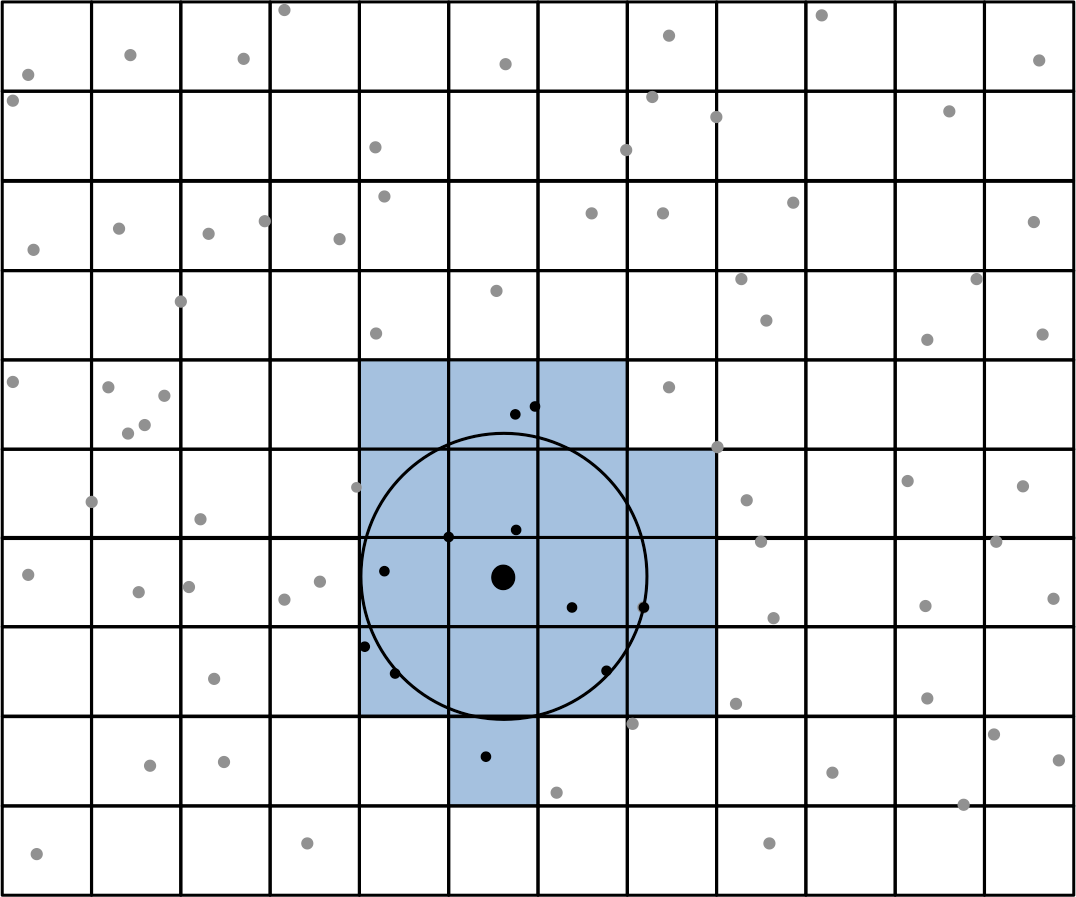
\includegraphics[width=0.6\textwidth]{figures/grid4_crop.png}
\caption{This illustrates, in two dimensions, the grid based spatial indexing method.
The naive S-GB method would require a distance computation to every other atom in the system.
By only considering atoms in cells intersecting the radius of influence, represented here in blue, it is possible to consider far fewer interactions.
Although only atoms inside the circle in this illustration contribute to surface charge, it is necessary to compute the distance over all black points.
Without using this hashing scheme, it would be necessary to compute the distance to each gray point as well.}
\label{figure:grid_hash}
\end{center}
\end{figure}


    \subsection{Experiments}
    \label{subsection:experiments}
    % side chain prediction experiments
For side chain prediction, the specific side chains used were those which had at least 30\% solvent accessible surface area when evaluated in the absence of other chains or crystal neighbors.
Glycine and proline residues were also excluded, as they do not have free side chains.
Residues missing heavy atoms in the crystal structure were predicted; however, RMSD was not measured for these residues because there is no experimental data.
Side chain prediction experiments were performed as described in \cite{jacobson2002role}.

% energy calculations experiments
The experiment in this case consisted of multiple energy calculations, using the modified version of the OPLS-AA force field described in \cite{li2011vsgb}.
In the control experiments, the same method for evaluating the implicit solvent term was used as in previous works.




\section{Results}
\label{section:cell/results}
\subsection*{Qualititave Measures of Prediction Quality}
\label{subsec:results_quality}

For side chain prediction experiments, 85.2\% of side chain prediction conformations (9406 of 11030 total) predicted with the new cell based solvation model are within 0.2 angstrom heavy atom RMSD of the prediction using the naive implementation.
In other metrics, the quality of prediction is comparable between the two solvent models. 
Median side chain heavy atom RMSD is 0.567 and 0.558 angstroms for the cell based method and the non-cell based method, respectively.
Average RMSD to the crystal structure is similarly close, 1.11 angstroms for both methods, with 79.9\% of side chain predictions within 2 angstroms RMSD of the native using the cell based model and 79.4\% within two angstroms using the naive approach.
Of side chains which are predicted differently by the two implementations there is no correlation between solvation model and prediction quality.
The distribution of side chain predictions with respect to RMSD to native is also indistinguishable between the two methods of computing the solvation term.

Data for energy calculations is not presented here because it is identical in every case.
This is expected, given that the two models represent two methods of computing the same quantity.
Thus, on the whole, prediction accuracy of the hash based model is comparable with the old implementation.

\subsection*{Performance Improvement}
\label{subsec:performance_improvement}
The principal goal of the hash based approach is to improve the performance of the implicit solvent models. 
Thus, the key metric of performance improvement is the speedup over the previous implementation.
Energy computations were found to be from 1.6 to 2.5 times as fast, and the trend indicates that even larger improvements would be obtained in larger system.
This sort of experiment represents a ``best case'' for the expected performance increase of a hash based solvent, as they represent a minimum amount of time spent on other parts of the experiment.
Implicit solvent calculations, and energy calculations in general, compose a smaller fraction of time in simultaneous side chain prediction therefore the observed performance improvement is less than that of energy calculations.
The observed performance increase in this sort of experiment is still on approximately 20\%.

\begin{figure}[H]
\begin{center}
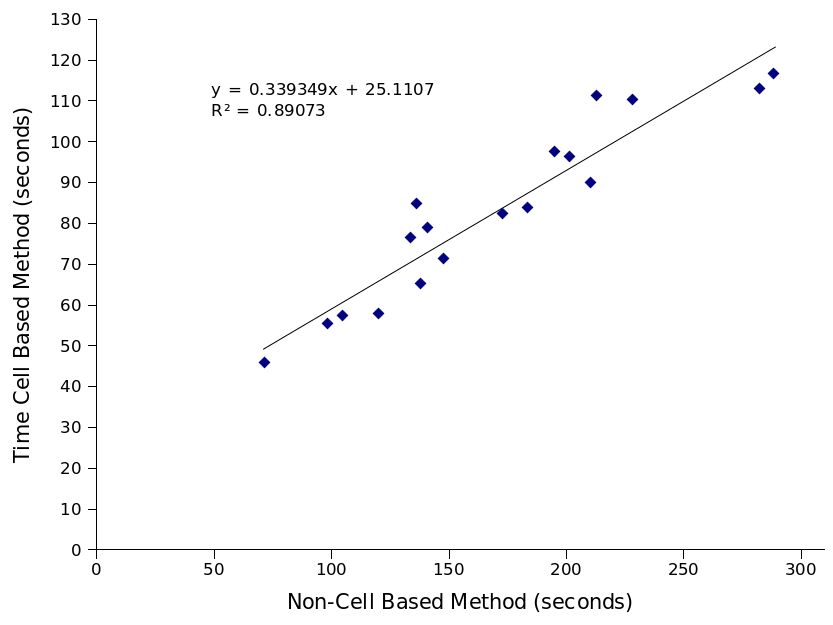
\includegraphics[width=0.8\textwidth]{figures/energy_calculation_timings.png}
\caption{Energy computations using a grid based method yields approximately a three times performance improvement, though in the case of some very small structures it is possible that the overhead introduced by maintaining the grid structure outweighs the improvement.}
\label{fig:ddr}
\end{center}
\end{figure}

\begin{table}[H]
\centering
\label{table:energy_timings}
\begin{tabular}{|c|c|c|}
\hline
PDB id	& Naive Method	& Cell Based Method	\\
\hline
1F5Z	&   201.75	&   96.37	\\
1H2V	&   98.31	&   55.32	\\
1HRD	&   228.38	&   110.12	\\
1M1Z	&   147.83	&   71.28	\\
1M9X	&   282.35	&   113.04	\\
1O60	&   172.82	&   82.34	\\
1R0V	&   210.35	&   90.0    \\
1XMP	&   213.25	&   111.25	\\
2E3Z	&   141.11	&   78.79	\\
2H6U	&   138.25	&   65.07	\\
2OU1	&   104.93	&   57.24	\\
2XI9	&   71.68	&   45.73	\\
3AMD	&   288.58	&   116.52	\\
3DEL	&   133.62	&   76.48	\\
3E1E	&   183.8	&   83.8	\\
3FGN	&   120.38	&   57.75	\\
3HHP	&   195.25	&   97.58	\\
4GVR	&   136.35	&   84.78	\\
\hline
\end{tabular}
\caption{The specific timings for a series of energy computations presented in Figure \ref{fig:ddr}.
These represent a ``best case'' scenario, as the majority of time in these experiments is spent computing the solvent contribution.}
\end{table}
% Would it be useful in this table to add a column that shows %improvement?






\section{Discussion}
\label{section:cell/discussion}
%Summarize what you did and results
We have developed an application of a classic computer science grid based hashing algorithm to the implicit solvent model of PLOP.
We demonstrate that this application does not affect accuracy of results compared with the previous implicit solvent model implementation in PLOP.
Though in a small number of cases side chain conformations are predicted in widely different conformations by the hash based method and the old implementation, the two methods are equally likely to predict the more native-like structure, so this variance can be attributed to noise.
We have also found in other experiments that the final predicted structure of a minimization is very sensitive to both small changes in pre-minimization coordinates, of a magnitude far less than bond distances, and minimization parameters.
It possible that these effects magnify small differences present early in the experiment, resulting in much larger differences between the final predicted structures.
Finally, we present data showing that the reduced computational cost of evaluating the solvent contribution using this hash based approach dramatically reduces the total time spent evaluating the energy model by a factor of 1.6 to 2.5.

% talk about hash method, 
Note that any such geometric hashing will introduce some overhead for maintaining the data structure.
As discussed by Bentley and Friedman \cite{bentley1979data}, the total storage necessary for the hash structure and the time necessary to sort atoms into cells are both linear in the number of atoms, and placing or updating a single atom in the structure is a constant time operation.
The improvement in retrieval using this structure dominates the cost of maintaining the structure, and the difference becomes more pronounced as system size grows.
Bentley and Friedman also present a through review of the performance characteristics of a number of other geometric hashing techniques, though they compare the algorithms in a data agnostic means.
Taking advantage of the characteristics of physical data, in this case atomic coordinates, has some effect of the relative advantages and disadvantages of specific hashing techniques. 
Specifically, the maximum number of atoms per cell is limited by physical constraints of atomic interactions.
% other hashing methods - octree.  why yours is better
An octree is a similar, though hierarchical, hash structure used in computer graphics for fast location based retrieval.
However, because the criteria for ``collision'' in this case is a fixed distance cutoff, and the data is roughly uniformly distributed it is efficient to used a fixed cell size\cite{turk1989interactive}.

% Can be implemented anywhere there is a pair interaction term
Though the implicit solvent term was initially targeted, because it dominates the time spent in energy calculations, it is possible to apply this method to any pair-pair interaction.
Though especially for shorter range interactions it might be beneficial to either maintain a higher resolution hash, or implement a hierarchical spatial hash, such as an octree.
We are also applying this geometric hashing technique to collision detection between simultaneous loop predictions.
This will allow efficient screening of neighboring loop prediction candidates, which will be particularly useful in predicting structures with multiple nearby solvent exposed loops, such as G-protein coupled receptors.

% implicit/explicit comparison discussion
Implicit solvation models offer a very tangible benefit over explicit solvent models, both in performance and experimental complexity.
Though explicit solvation is sometimes viewed as a ``gold standard'', it has been shown that current implicit solvent models can, at least sometimes, reproduce predictions of explicit solvent models.
However, development of implicit solvent models is important since improved performance compared with explicit solvent methods allows modeling of larger systems, longer timescales, or improved sampling.
The complexity of the experiment is also reduced, using implicit solvent models, because results are not dependent on sampling of water conformations in addition to protein conformations.
However, implicit solvent models can still be very computationally expensive.
For instance, in the PLOP implementation of the OPLS-AA energy model with SG-B solvation term, evaluating the solvation term consumes up to 80\% of the total time spent in energy calculations, dependent on size of the symmetric system.
This is in large part due to the time complexity of evaluating the SG-B solvation term.
Thus an algorithm that offers further reduction in experimental cost without a tradeoff in accuracy represents valuable progress in the development of implicit solvent models.


%%%%%%%%%%%%%%%%%%%%%%%%%%%%%%%%%%%%%%%%%%%%%%%%%%%%%%%%%%%

% practical considerations and limitations
Because the size of protein systems are limited, at some level, by physical limits, the maximum system size expected to be encountered is limited.
Therefore, although the new method reduces the time complexity of implicit solvent calculations, the maximum expected speedup is limited to about a factor of three in large systems.
The actual speedup depends on both the system size, and the amount of time that a given experiment spends evaluating the solvent contribution.
The speedup observed in side chain prediction experiments was much less, around 20\%, though it is possible that applying a similar method to terms of the gradient during minimization would increase that amount.
Nonetheless, even a 20\%  speedup represents a significant improvement, especially as structure prediction methods continue to depend on parallel prediction and reprediction of the same region as a method of structure refinement\cite{goldfeld2013loop}.
% could be future work
Although this algorithm improves on the theoretical time complexity of the S-GB implicit solvent model, parameterization such as the number, and size of cells in the grid structure could have a significant effect on run time.
Some effort was made towards choosing reasonable parameters, but they are likely not optimal.
Hardware that is optimized for this sort of spatial indexing and collision detection, or proximity detection, exists in modern video cards, and along with general purpose programming for this sort of hardware it should be possible to further parallelize computation of implicit solvation effects for even greater performance improvements\cite{harris2008cuda}.

\subsection*{Acknowledgements}
\label{subsec:acknowledgements}
Experiments were performed by J.B. over the last year at the Columbia University Chemistry Department cluster on a mix of hardware. 
J.B. is funded by XXXX.
R.F. is funded by XXXX. R.F. has a significant financial stake in Schr\"{o}dinger, Inc., is a consultant to Schr\"{o}dinger, Inc., and is on the Scientific Advisory Board of Schr\"{o}dinger, Inc.



\chapter[Computational Mutation Scanning]{Progress in Computational Mutation Scanning}
\label{chapter:mutation}

\section{Introduction}
\label{sec:mutation/intro}
In order to determine which amino acids in a protein play the largest role in determining binding affinity it is convenient to compare the binding affinity of the native protein with that of a single residue mutant.
If the change in residue does not affect the folding of the protein, which with the exceptions of mutations to glycine, proline, or depending on the local structure possibly large amino acids, is unlikely. 
Alanine is the most frequently occurring amino acid, appearing in both solvent exposed and buried positions \cite{chothia1976nature,rose1985hydrophobicity}, and is unlikely to disrupt the protein fold in the same way glycine or proline might \cite{klapper1977independent}.
Additionally because it lacks a charge it does not interact electrostatically with the ligand.
These reasons makes it an attractive choice as a ``control'' amino acid for mutation scanning experiments.
Mutation scanning experiments, seek to identify residues which are have the largest contributions to binding affinity or ``hot spot'' residues.
By identifying single residue mutants which have a significantly decreased binding affinity when mutated to alanine \cite{cunningham1989high}.
\begin{figure}[h]
\centering
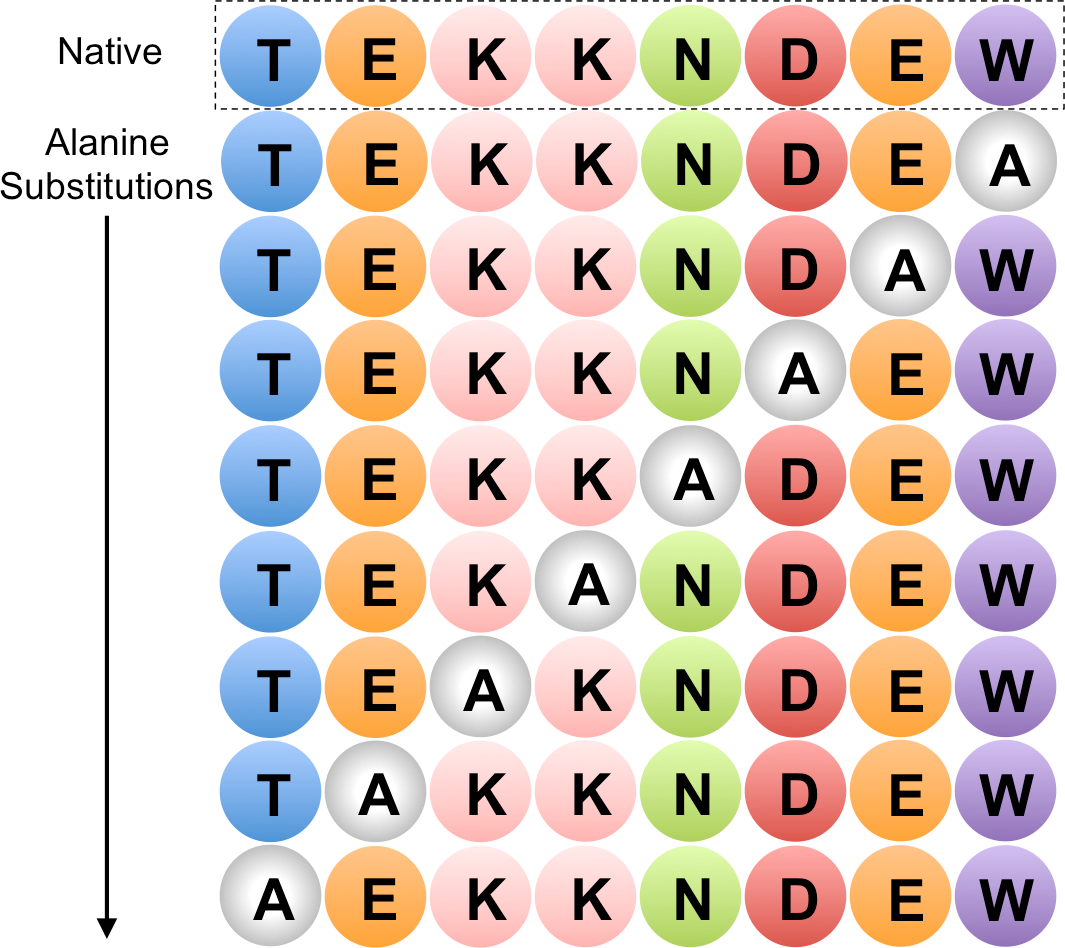
\includegraphics[width=0.5\textwidth]{figures/alanine_scan.png}
\caption{The sequences which would be evaluated during an alanine scan for Fc domain of a human IgG for streptococcal protein G.
The residues identified here were taken from the AESDB.
The native protein is represented in the top row \protect\cite{sauer1995crystal,thorn2001asedb}.
}
\label{fig:alanine_scan}
\end{figure}

The immune system maturation response, selects antibodies which have a reasonable affinity for an antigen, and creates a large number of variants of these antibodies. 
The effect of this is that the body produces antibodies with increasing affinity for an antigen some time after the initial exposure \cite{griffiths1984somatic}.
In vitro affinity maturation attempts to select molecules, frequently antibodies, with high affinity for some target molecule by creating a library of bacteria displaying variants of these antibodies on their cellular surface.
The means of doing this is bacteriophage display, which provides a method of pairing the protein represented on a bacterias surface with the genetic material contained by that bacteria \cite{smith1985filamentous}.
A bacteria is infected by a library of bacteriophages, containing a large number of variants of antibody of interest.
The phage will cause the bacteria to display their specific variant of the antibody on the bacteria surface, allowing sorting of the bacteria according to their affinity of the antigen, though affinity column purification or similar technique.
This step greatly enriches the fraction of antibody variants which bind the protein.
It is then possible to allow the bacteria to reproduce, sometimes causing more mutations to increase diversity of the antibody library and perform this affinity purification step again.
Sequential application of this affinity maturation makes it possible to identify a handful of antibody variants with high affinity from as many as $10^{6}$ different variants \cite{gram1992vitro,hawkins1992selection}.
However, the number of possible variants of the complementarity determining region (CDR) of an antibody many orders of magnitude larger than this.

Computational mutation scanning attempts to replicate the same sort of experiment {\it in silico}.
Making the same assumptions as above, namely that the backbone conformation is not altered by mutating a single residue to alanine, computational experiments attempt to identify hot spot residues by measuring the \ddg\ between the bound states of the native and mutated protein.

Mutated structures were generated by truncating side chain at C\subscript{$\gamma$} 
\cite{massova1999computational}

Varying cutoffs for {\it hot spot} residues are used, usually from 1.0 kcal/mol \cite{kortemme2002simple} to 4.0 kcal/mol \cite{pons1999energetic}.

Mutations at these {\it hot spot} residues tend to be strongly deleterious leading to above average conservation  \cite{hu2000conservation,lichtarge1996evolutionary}.

% computer aided antibody design \cite{kuroda2012computer}
%\cite{moreira2007computational}

\subsection{Entropy-Enthalpy Compensation}
Some computational alanine scanning experiments explicitly compute or approximate the entropic contribution to the change in the free energy of binding \cite{hao2010computational,guerois2002predicting}. 
However, other models have achieved good agreement with experimental data while assuming these effects are either accounted for by the correlation between entropy and enthalpy for small changes in protein structure \cite{sharp2001entropy} or to be small relative the entropic changes \cite{kortemme2004computational}.
PLOP has not made use of entropic contributions to free energy and has in many cases achieved good agreement with experiment, so in these experiments it is assumed that contributions due to entropy are small relative entropic contributions.



\section{Methods}
\label{sec:mutation/methods}
\subsection{General Mutation Screening}
The generalized mutation screening method implemented in PLOP allows efficient evaluation of a large number of possible mutations.
It accepts as input a set of possible mutations for each residue, or a set of possible mutations for a set of residues.
For instance tryptophan, tyrosine and arginine are overrepresented in hot spot resiudes \cite{hu2000conservation}, so it may be desirable to consider all mutations in which a set of residues are either left at their native identity or replaced with one of these residues.
If desired the user can also set bounds for the minimum and maximum number of simultaneous mutations allowed.
The residues which will be mutated are referred to as {\it free} residues as the conformations of the other residues are held fixed throughout the entire process.
While the residues are still in their native states the structure is subjected to some sort of sampling.
This is done in order to prevent bias towards predicted states which will later be predicted in the same fashion.
In the present implementation this consists of predicting the conformation of each free residue is minimizing those residues.

In this side chain sampling, for each free residue, the sidechain is initially replaced with a random conformation from a high resolution rotamer library screened for steric clashes with the static part of the protein.
The free residues are then examined sequentially replacing each with the lowest energy conformation present in the rotamer library.
This replacement process is continued until the termination condition is met, which is that two or fewer residues are replaced by lower energy conformations during the replacement stage.
Five iterations of this procedure, from randomization to a static conformation, are performed and the most frequently selected conformation is chosen for each amino acid \cite{jacobson2002force,jacobson2002role}.

In the mutation stage, each free residue is first updated to its new chemical identity, possibly remaining in the native state, sidechains are replaced with the sidechain of the desired amino acid, with the corresponding updates to the bond, angle, torsion, and 1-4 interactions.
The conformations of free residues are then re-predicted using the same side chain prediction algorithm described for the native conformation.

\subsection{Alanine Scanning Experiments}
Three protein complexes, 1FCC, 1BRS, and 1DVF, with both experimental data for binding affinity and crystal structures were identified using the ASEdb \cite{thorn2001asedb}.
Protonation states and locations of polar hydrogens were assigned for all residues as in \cite{li2007assignment}.
A crystal context was built for each structure using symmetry data determined by experiment.
For each mutation represented in the alanine scan database single residue was mutated to alanine and this side chain prediction was repeated.
The resulting structures were examined side chain conformation agreement with crystal structures and the change in binding free energy to native was recorded. 


\section{Results}
\label{sec:mutation/results}
A strong correlation between observed and expected \ddg\ was not found for any of the structures nor for the set of mutations taken as a whole.
Despite this single side chain conformations were in very good agreement between predicted side chain locations and crystal structures, suggesting that sufficient sampling was done in the side chain prediction step.
\begin{figure}[H]
  \centering
  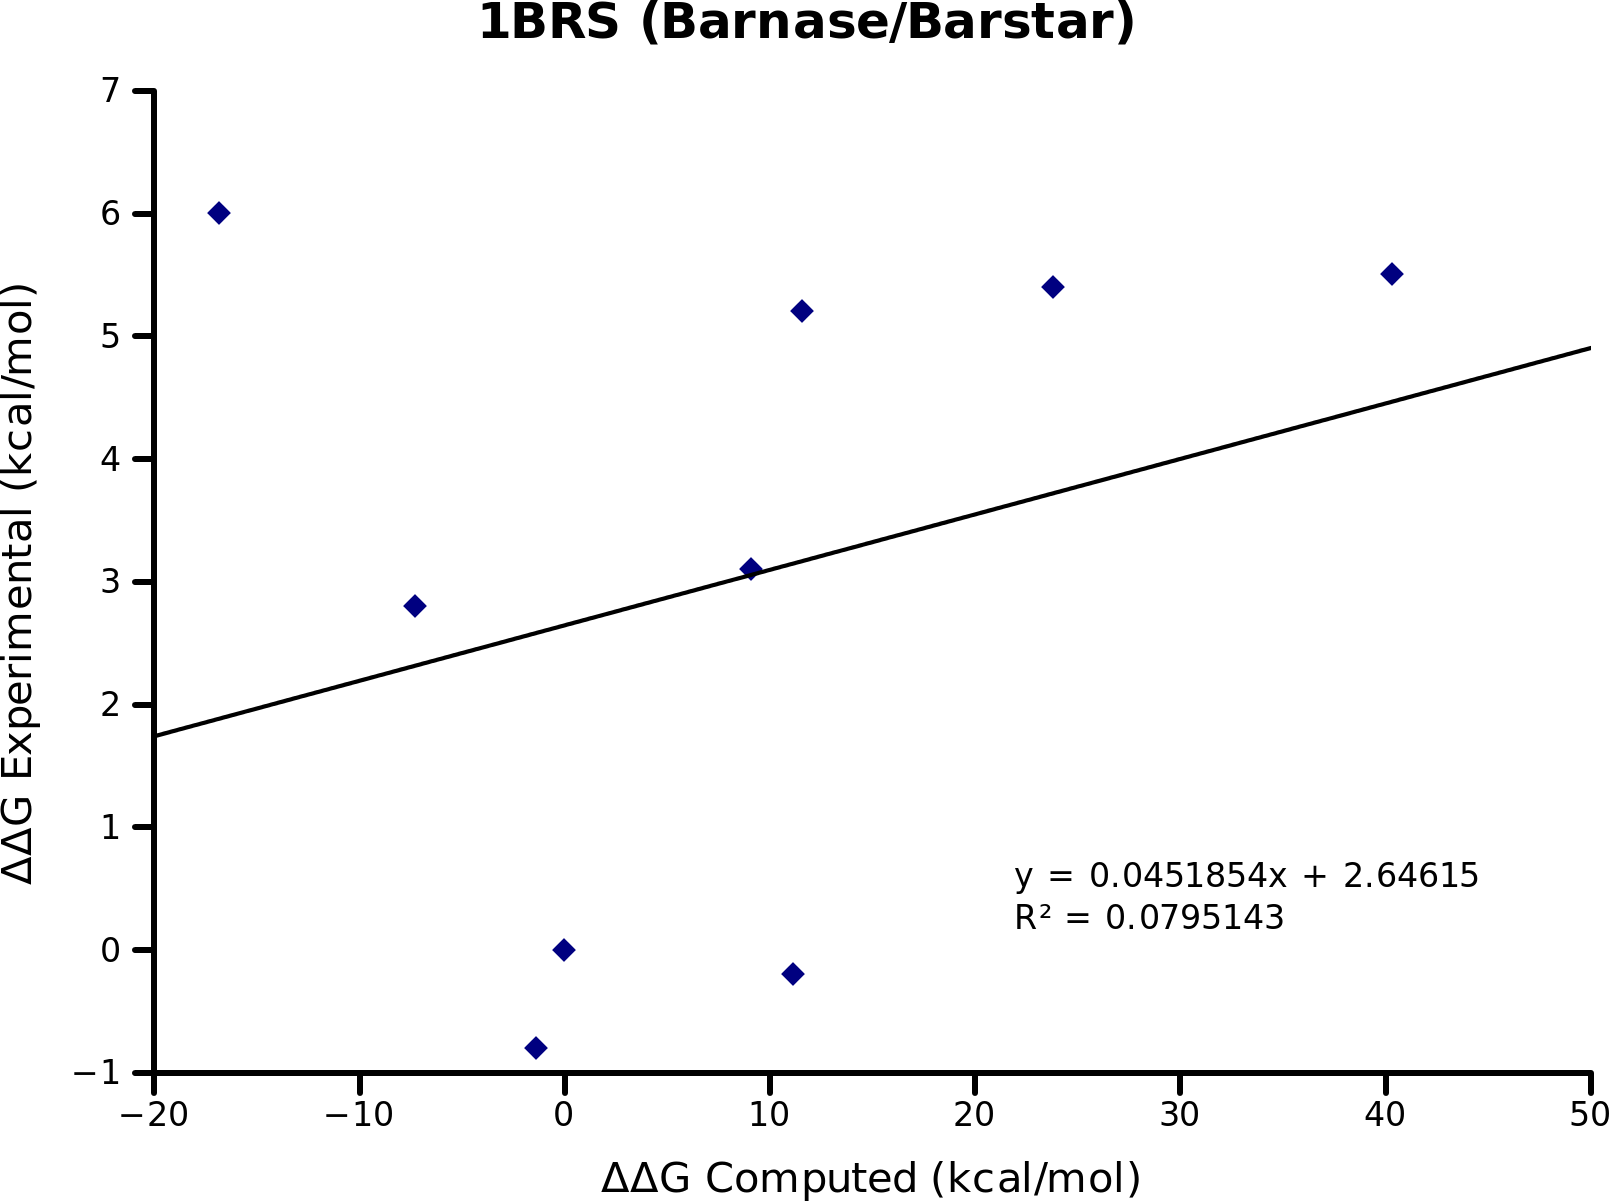
\includegraphics[width=0.65\textwidth]{figures/1brs_barnase_barstar.png}
  \caption{
Computed versus experimental \ddg\ binding for 8 alanine mutations in the Barstar-Barnase binding pair.
Crystal structure used for computations was 1BRS.
Specific amino acids mutated were residues 27, 54, 58, 59, 60, 73, 87, and 102, all of chain A.
Experimental binding affinity taken from \protect\cite{thorn2001asedb}.
            }
\end{figure}

\begin{figure}[H]
  \centering
  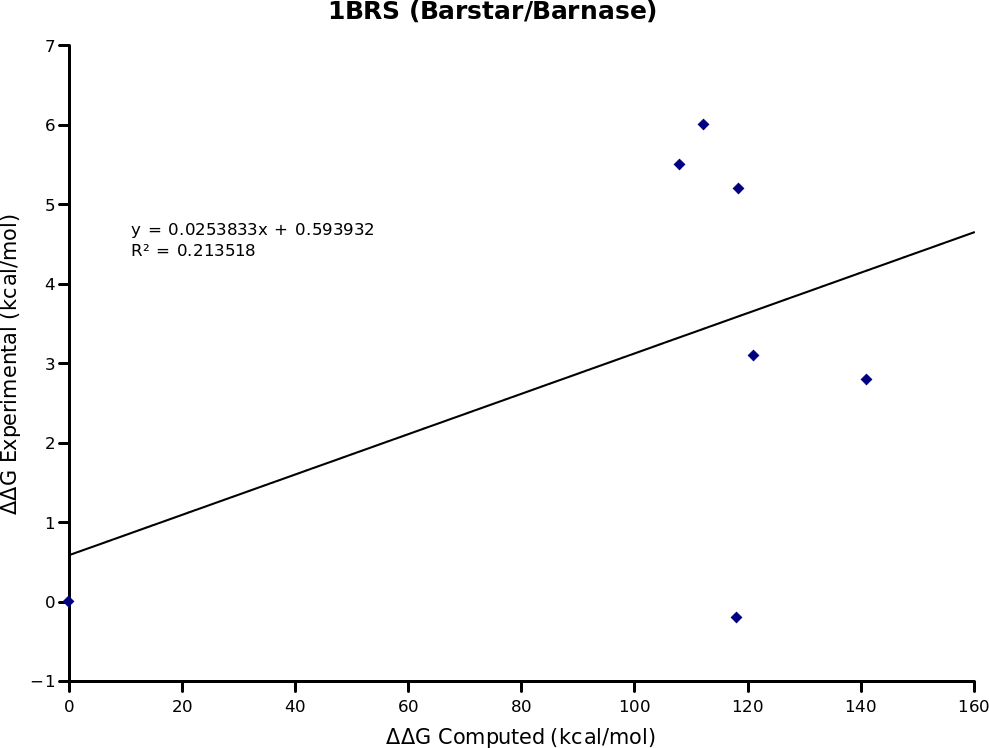
\includegraphics[width=0.65\textwidth]{figures/1brs_barstar_barnase.png}
  \caption{
Computed versus experimental \ddg\ binding for 6 alanine mutations in the Barstar-Barnase binding pair.
Crystal structure used for computations was 1BRS \protect\cite{buckle1994protein}.
Specific amino acids mutated were residues 29, 35, 39, 42, 74, and 78, all of chain D.
Experimental binding affinity taken from \protect\cite{thorn2001asedb}.
            }
\end{figure}

\begin{figure}[H]
    \centering
  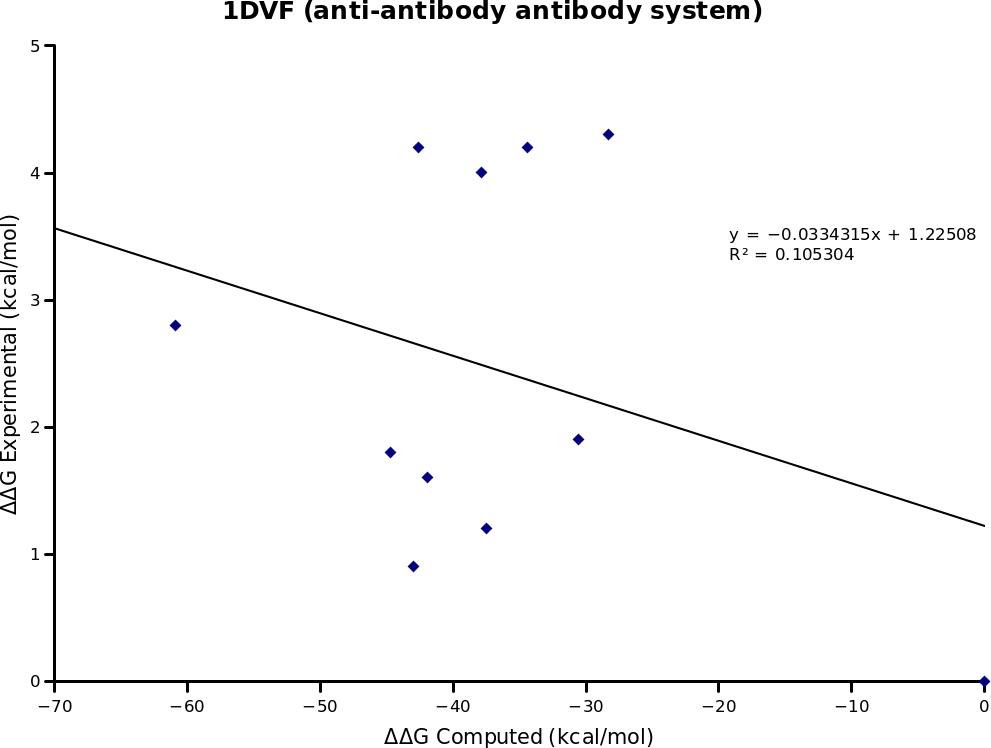
\includegraphics[width=0.65\textwidth]{figures/1dvf.png}
  \caption{
Computed versus experimental \ddg\ binding for 10 alanine mutations in the anti-hen-egg-white lysozyme antibody (D1.3) anti-idiotopic antibody (E5.2) complex.
Crystal structure used for computations was 1DVF \protect\cite{braden1996crystal}.
Specific amino acids mutated were residues 30, 32, 52, 54, 56, 58, 98, 99, 100, and 101, all of chain A.
Experimental binding affinity taken from \protect\cite{thorn2001asedb}.
            }
\end{figure}

\begin{figure}[H]
    \centering
  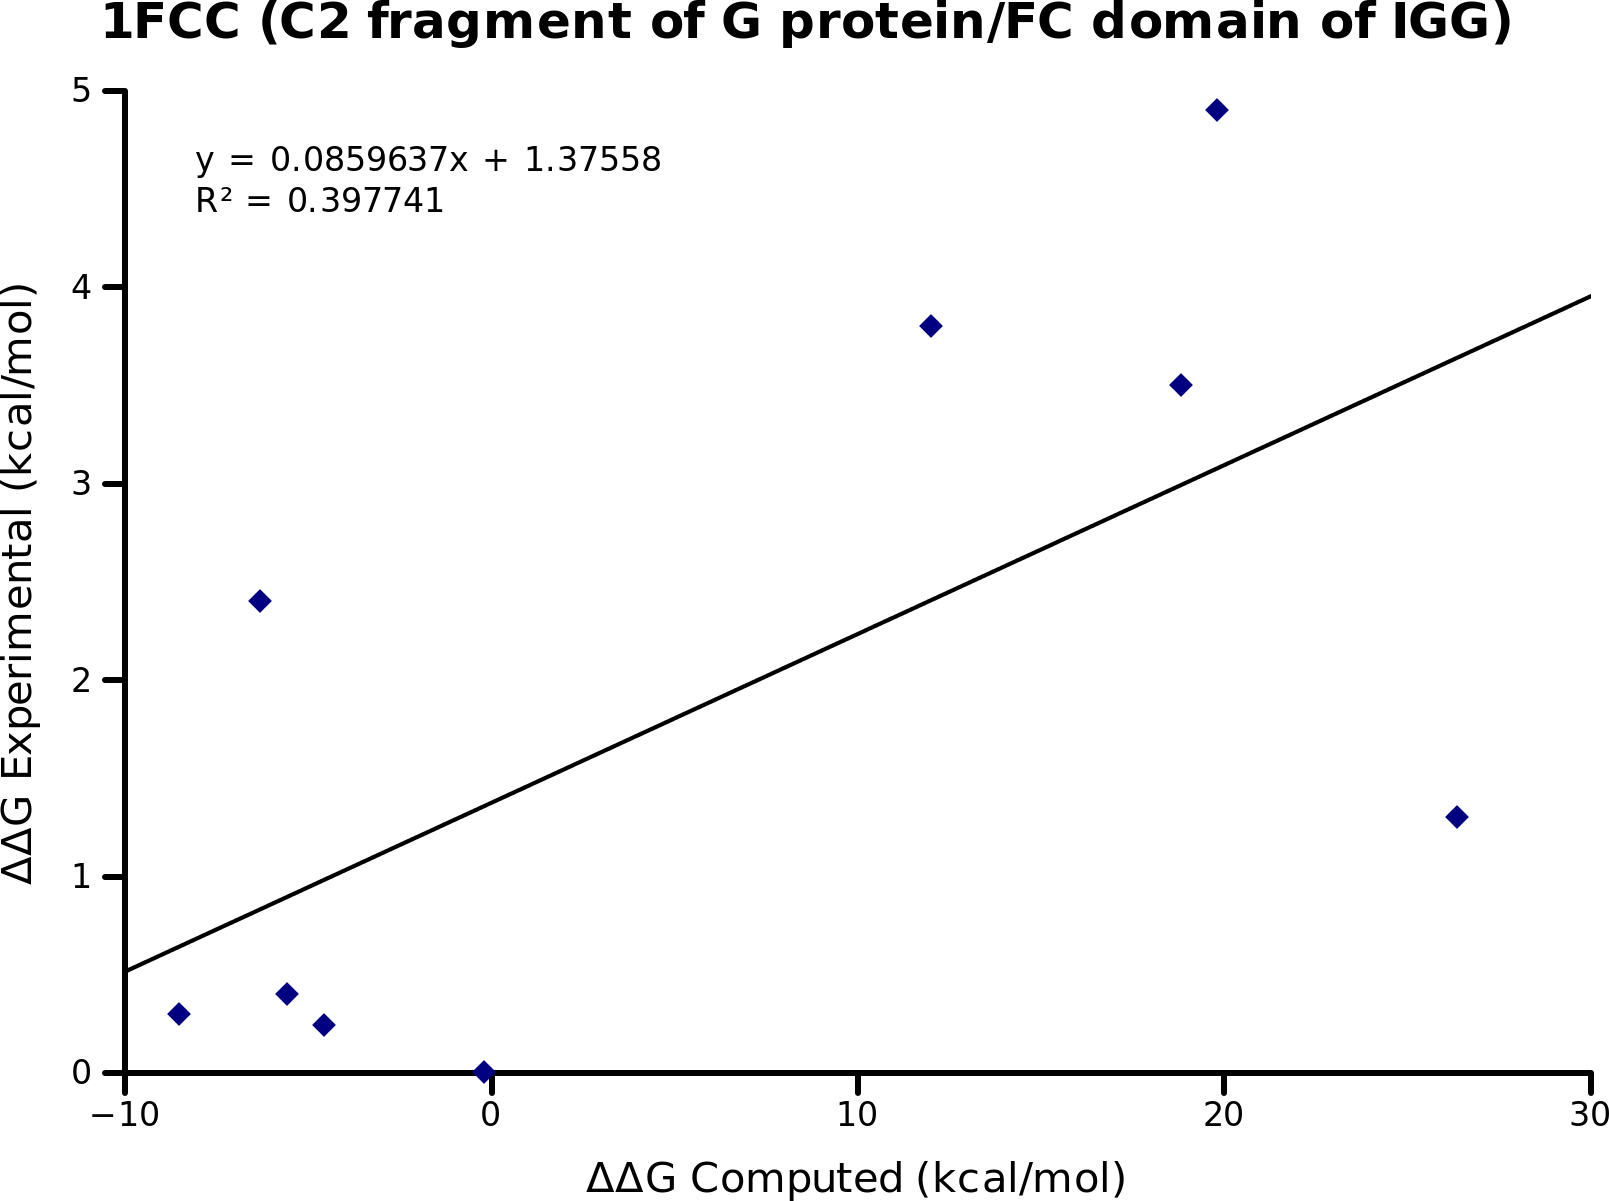
\includegraphics[width=0.65\textwidth]{figures/1fcc.png}
  \caption{
Computed versus experimental \ddg\ binding for 8 alanine mutations in  binding pair.
Crystal structure used for computations was 1FCC.
Specific amino acids mutated were residues 25, 27, 28, 31, 35, 40, 42, and 43, all of chain A.
Experimental binding affinity taken from \protect\cite{thorn2001asedb}.
            }
\end{figure}



\section{Discussion}
\label{sec:mutation/discussion}
There are two necessary subproblems in accurately predicting the effect of mutations on local protein structure:
\begin{enumerate}
\item prediction of side chain conformations, and
\item accurately describing the energetics of the interactions.
\end{enumerate}
In the work presented here, we have shown that our current methods are able to accurately predict side chain conformations of mutated residues, discussed below in \ref{subsection:side_chain_prediction_accuracy}.
However, it seems that despite being able to differentiate between native and non-native side chain conformations, we are unable to correlate experimental changes in binding energy with computational predictions.
Possible reasons for this discrepancy are addressed in subsection \ref{subsection:energetic_correlation_with_experimental_data}.

\subsection{Side Chain Prediction Accuracy}
\label{subsection:side_chain_prediction_accuracy}
Our results indicate that we are able to successfully predict side chain conformations on protein interfaces in the majority of cases examined.
Specifically, 29 of 32 side chains predicted over four chains in three independent structures are within 1.5 angstroms of the native conformation, with a significant number of side chains predicted closer to the native crystal conformation than the resolution of the crystal structure.
This indicates that both the sampling performed here and the energy model are sufficiently extensive and accurate to reproduce the native conformation, which has been used as a standard metric of success in many previous studies, e.g. loop predictions \cite{jacobson2004hierarchical,rapp1999prediction,zhu2006long,sellers2008toward} and side chain predictions \cite{jacobson2002force,jacobson2002role,zhu2007improved}.
One of the reasons that RMSD is so popular as a performance metric is the difficulty of obtaining experimental data that can be directly compared to experimental predictions.
Binding affinity studies, especially alanine scanning experiments, represent a wealth of data that might be used in training more accurate next generation molecular mechanics energy functions.


\subsection{Energetic Correlation with Experimental Data}
\label{subsection:energetic_correlation_with_experimental_data}
We found that despite predicting side chain conformations approximately correctly, there was generally no correlation between our computed \ddg\ and the experimental \ddg\ from the alanine scanning database.
The relationship between experimental and computationally predicted \ddg\ can be seen in figures \ref{figure:computational_mutation_scanning/1BRSa_ddg}, \ref{figure:computational_mutation_scanning/1BRSd_ddg}, \ref{figure:computational_mutation_scanning/1DVF_ddg}, and \ref{figure:computational_mutation_scanning/1FCC_ddg}.
It is somewhat surprising that side chain predictions are as accurate as they are without any real correlation in binding affinity.
A common assumption is that accuracy of predicted conformations implies accuracy of the energy model.
However, this depends on very extensive sampling, such as in full molecular dynamics simulations.
It is possible for biased sampling, such as is performed here with the goal of both increasing accuracy and speed of exploring conformation space, to mask shortcomings in an energy model.

Experiments by other groups have demonstrated some success in correlating computational \ddg\ with experimental \ddg\ \cite{kortemme2004computational}.
Some of these experiments have made use of energy models that are largely similar to the one implemented in the PLOP program.
Despite this, we did not find a significant correlation between experimental data and predictions with respect to \ddg.
It is possible that the interactions at a protein-protein interface are somehow different than intramolecular interactions, which have constituted the majority of the training sets used to develop the PLOP energy model.

Additionally, some hot spot residues are tightly constrained in conformation by neighboring protein structure, making prediction more similar to placing a jigsaw piece than searching for a low energy conformation among many possibilities.
This sort of situation was especially prevalent in tyrosine 43 of 1FCC.
In this case there were only two conformations from the side chain rotamer library that were not eliminated in the initial screening process.
The conformation of tyrosine 43 in the protein context is shown in \ref{figure:1fcc_43_pocket}.

Finally, because the rotamer library used here biases sampling towards experimentally observed side chain conformations, it is possible that the energy model is capable of correctly ranking conformations present in the library by energy, but it performs less well for areas of conformational space outside the rotamer library.
In order to test this hypothesis it would be necessary to use a non-rotamer based approach in a similar set of experiments.
Conveniently, the side chain sampling method used in the minimization Monte Carlo experiments described in chapter \ref{chapter:p450} can be used to perform such an experiment.

\subsection{Future Directions}
% where is the error coming from sampling/energy
Current data indicates that the sampling method introduced here is sufficiently exhaustive to identify native like conformations.
Thus, it would be logical for future work to focus initially on exploring and improving the energy model.
As mentioned above, one possible means of doing this would be to implement an energy model used in similar experiments, such as CHARMM, used by the Baker lab in their hot spot identification experiments, in which they were able to successfully predict hot-spot residues, and those that did not contribute significantly to the binding affinity \cite{kortemme2004computational,lazaridis1999effective}.
This would allow for testing of the sampling method independently of the energy model used, to support the success of or reveal potential shortcomings in the sampling method.

% energy model accuracy
Testing the performance of the energy model on protein-protein surfaces and classifying the errors would be a necessary step in improving the correlation between predicted and experimental \ddg.
It would also be very enlightening to be able to compare the performance of the PLOP sampling methods using a known energy model implemented in a different molecular mechanics toolkit.

% sampling modular allows for flexibility
The sampling introduced in these experiments is very modular in nature.
Because of this, it would be possible to modify the sampling procedure used in the code, or even to specify the sampling method in the input file.
This flexibility will hopefully allow testing of many different sampling methods in order to find a method that provides a good balance of time and coverage of conformational space.

Because the method implemented here is capable of not only alanine scanning, but also generalized mutation scanning, it is possible to computationally screen interactions between a large number of variants of similar proteins.
If the correlation between predicted and experimental binding affinities can be further improved, there would be a number of extremely valuable applications for such a method.
First, it would be possible to screen variants of an antibody in order to help accelerate affinity maturation.
Second, it might also be possible to test the efficacy of a number of drugs targeting highly variable proteins, such as HIV protease \cite{watkins2003selection}, by screening the drug against a number of possible mutations.



\chapter[p450 Sites of Metabolism]{Prediction of p450 Sites of Metabolism}
\section{Introduction}
\label{section:p450/introduction}
The most common method of drug clearance among currently perscribed drugs is metabolism, which is the primary method of clearance for approximately 75\% of the top 200 most commonly perscribed drugs in the United States \cite{williams2004drug}.
Cytochrome p450 is critical to drug metabolism, being active in approximately 75\% of drugs which are cleared in this method \cite{guengerich2007cytochrome}.

\begin{figure}[h]
\centering
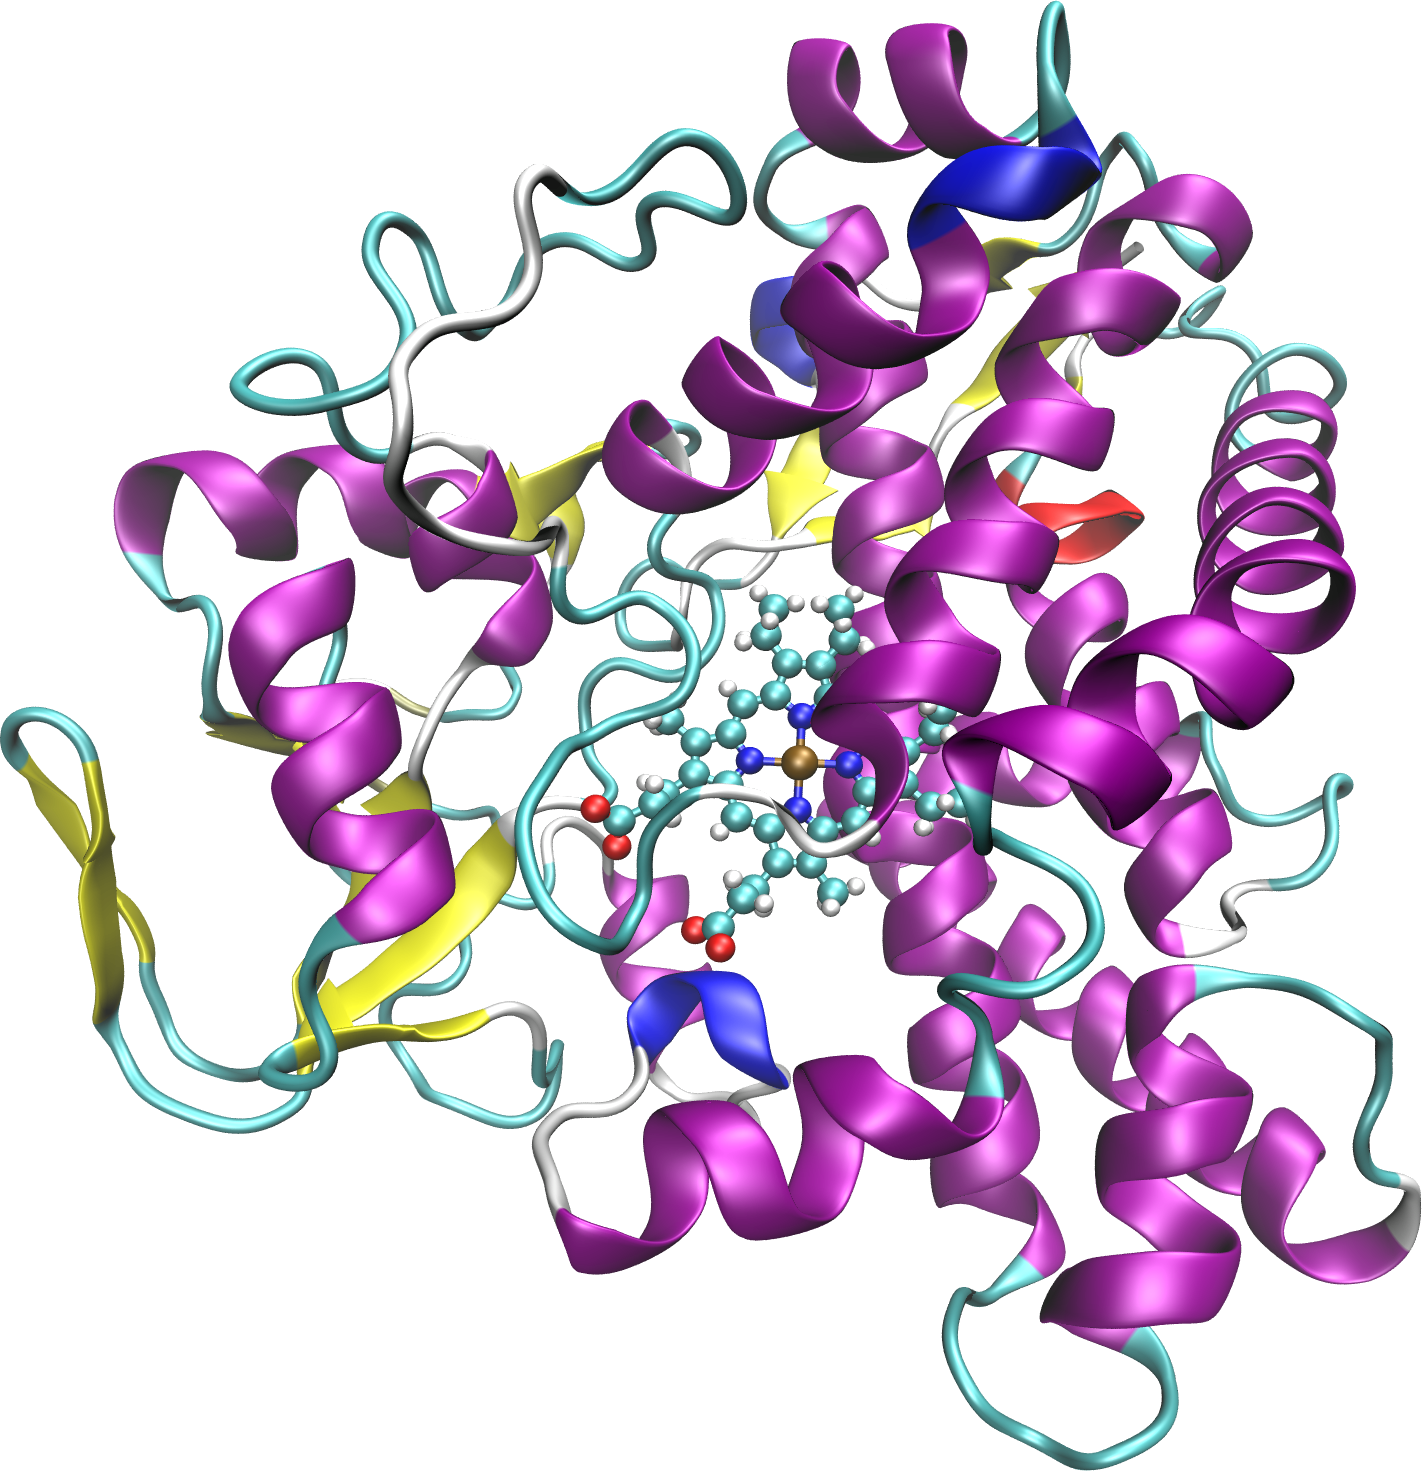
\includegraphics[width=0.5\textwidth]{figures/p450.png}
\caption{
The structure of cytochrome P450, taken from PDBid 1JFB, shown in cartoon representation.
The bonded heme group, shown as ball and stick model, is visible in the center.
}
\label{fig:p450}
\end{figure}


\section{Methods}
\label{section:p450/methods}

\begin{figure}[h!]
\centering
\includegraphics[width=0.55\textwidth]{dot_files/idsite.png}
\caption{An overview of the entire IDSite procedure.
The dotted lines represent abbreviated versions of the full procedure.
Receiver operating characteristic graphs for the full version, and these abbreviated versions, are presented in \ref{figure:idsite_roc_sampling}.
Series colors on ROC graphs correspond to arrow colors here.}
\label{figure:idsite_overview}
\end{figure}

Prediction of sites of metabolism is a three stage procedure:
\begin{enumerate}
\item Initially a number of different ligand conformations are generated, and these are docked into a rigid protein, with soft VDW terms using Glide \cite{halgren2004glide,friesner2004glide}.
\item The docked conformations are refined using a Monte Carlo Minimization (MMC) approach which samples degrees of freedom in both the ligand and protein.
\item Refined conformations are classified into reactive site or non-reactive site on the basis of the energy of the refined conformations and the intrinsic reactivity of the site. \cite{li2011idsite}
\end{enumerate}

\subsection{Docking}
\label{subsection:p450/docking}
In the initial docking stage of the IDSite protocol Glide is used to generate a number of proposed docked conformations for each ligand.
Glide (standard precision) is used to generate a number of different ligand conformations by sampling conformations of freely rotatable bonds and rings.
A bounding box, which will be used for a grid search, is defined centered at the centroid of the ligand with an edge length of 10 angstroms.
Because the crystal structure used for CYP2D6 (PDBID: 2F9Q) does not have a ligand, the centroid of residues Glu216, Asp301, Thr309, and Phe483 was used instead in this case.
Because the steric clashes present in many proposed docked conformations can be relieved using a simple minimization procedure a reduced Van der Waals (VDW) radii are used in the docking stage for non-polar atoms.
The VDW radii used for the P450 are scaled by a factor of 0.4, and the scaling for the ligand starts at 0.8.
If an insufficient number of poses, in this case fewer than four, are found using these scaling factors for the radii the scaling of the ligand is stepped down until at least four poses are found.
Additional filtering of possible high energy conformations was also skipped in order to ensure the greatest diversity of docked poses reached the refinement stage.
The collection of docked poses are then clustered according to the RMSD of the ligand, and each pose is minimized.
The top sixty ranked poses according to the Glide SP metric are retained screened using a number of different criteria.
A hard sphere overlap criteria is used to remove poses with obvious steric clashes which were not removed during the minimization procedure.
A conserved feature of CYP2D6 ligand complexes is a salt bridge with Glu216 or Asp301.
In order to reduce sampling cost IDSite only considers structures with at least one hydrogen-bond donor within 4 residues of the centroid of these two residues and Ser304.
The sphere defined by these residues is illustrated along with the bounding box used for sampling in Figure \ref{fig:idsite_glide}
A number of other rule based geometric screens are used to remove structures which are unlikely to react.
Structures meeting any of the following criteria:
\begin{enumerate}
\item The distance of the basic nitrogen to the ferryl oxygen is less than 5.0 angstroms;
\item The distance of the basic nitrogen to the negative charged oxygen (in Glu216 or Asp301) is greater than 5.5 angstroms;
\item More than 2 heavy atoms from the ligands are further than 16.0 angstroms away from the heme iron;
\item More than 1 heavy atom from the ligand are closer than 1.0 angstroms to the receptor;
\item More than 6 heavy atoms from the ligand are closer than 1.8 angstroms to the receptor;
\item No heavy atom in the ligand is within 5.0 angstroms to the heme iron;
\end{enumerate}
are removed.
If the number of structures at this point is too low, the VDW scaling factors of the non-polar atoms of the ligand are stepped down, and the process is repeated.
If four or more poses are found at these point these poses are passed onto the next stage of the IDSite procedure, the Monte Carlo Minimization refinement stage.

\begin{figure}[h]
\centering
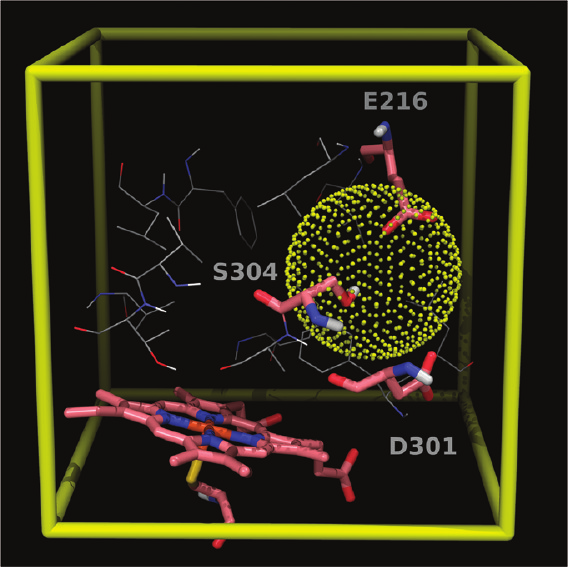
\includegraphics[width=0.35\textwidth]{figures/idsite/glide.png}
\caption{An overview of the entire IDSite procedure.}
\label{fig:idsite_glide}
\end{figure}

% IDSite uses reduced VDW radii for nonpolar atoms both in the protein receptor and the ligand, so that slight steric clashes are tolerated during the docking stage.
% For the protein receptor the VDW scaling factor is fixed at 0.40, while for the ligand, the scaling factor starting from 0.80 is adaptively adjusted until at least 4 valid poses are found.
% With highly flexible ligands and relatively high scaling factors, Glide often finds only a handful of valid poses, and even fewer survive after IDSite screening.
% However, if the scaling factor is set too low, the docked poses may contain too many serious steric clashes, which can cause problems in the subsequent minimization.
% If IDSite fails to find enough valid poses, the scaling factor is adjusted and the number of poses to pass the initial docking phase in Glide is increased accordingly to augment sampling.

% joe is this far
% If the ligand contains other hydrogen-bond donors except for the basic nitrogen, the constrained docking is likely to generate poses that form hydrogen bonds instead of the salt bridge to Glu216 or Asp301.
% However, IDSite is able to distinguish these poses and filter them via an additional salt bridge filter in the pose screening, so that only the poses with a stable salt bridge are allowed to pass to the refinement stage.


\subsection{Monte Carlo Minimization Refinement}
\label{subsection:p450/mcm}
Since the emphasis in IDSite sampling is efficient sampling of low energy conformations, as only the lowest energy conformations are passed on to the next stage of prediction, Monte Carlo Minimization was used instead of a more traditional Monte Carlo simulation because it provides more efficient sampling of low energy conformations (see \ref{subsection:monte_carlo}).
The Monte Carlo Minimization sampling used by IDSite for refinement incorporates three different types of steps: side chain motions, rigid body transformations, and hybrid Monte Carlo simulations.
For each Monte Carlo step, one of three types of motions is selected according to the weighted probabilities, which are different for the two different PLOP sampling stages (see table \ref{table:mmc_params}).
\begin{table}[h]
    \centering
    \begin{tabular}{|c|c|c|}
        \cline{2-3}
        \multicolumn{1}{r|}{~}                       & \multicolumn{2}{c|}{PLOP Sampling Stage} \\
        \cline{2-3}
        \multicolumn{1}{r|}{~}                       & First                        & Second                        \\
        \hline
        Number of Residues Sampled                   & 12                           & 40                            \\
        \vspace{-1.5ex}
        Number of Structures                         & \multirow{2}{*}{max(n*8,24)} & \multirow{2}{*}{max(n*20,60)} \\
        Advanced to Next Stage                       &                              &                               \\
        P(side chain step)                           & 0.5                          & 0.7                           \\
        P(rigid body step)                           & 0.1                          & 0.2                           \\
        P(HMC)                                       & 0.4                          & 0.2                           \\
        \hline
    \end{tabular}
    \caption{The number of residues sampled as well as the number of structures advanced to the next stage from each of the sampling stages.
Also, the relative probabilities of selecting each of the different sampling steps during a Monte Carlo minimization sampling stage.}
    \label{table:mmc_params}
\end{table}

Using the chosen method, a new conformation is proposed and minimized before the Metropolis acceptance criteria (equation \ref{equation:metropolis_acceptance}) is applied to the proposed state, using a temperature of 300 K.
All atoms of all residues with any atom within 5 angstroms of the ligand in the starting crystal structure were allowed to move during Monte Carlo moves, including the ligand itself.

During the minimization Monte Carlo sampling stages of the IDSite procedure, artificial constraints are used to guide the sampling towards a transition state like conformation.
These constraints create artificial bond or angle potentials, which affect the minimization but are not used in the Monte Carlo acceptance test.
For each of the minimization Monte Carlo sampling stages of the IDSite procedure, two different sets of constraints are applied depending on the hybridization of the carbon atom at the possible site of metabolism, for a total of four possible different sets of constraints.
In the first minimization Monte Carlo stage, two constraints are applied, shown in figures \ref{figure:first_sp2_constraints} and \ref{figure:first_sp3_constraints}:
\begin{enumerate}
\item The sulfur-iron-carbon angle is constrained to 145 degrees, with 20 degrees of ``slack'', or a flat bottom to the potential well (denoted as 145\plusorminus20 degrees).
The spring constant of this constraint is about 25 kcal/mol/degree\superscript{2}, or {\textapprox}40\% the strength of a carbon-carbon-carbon angle.
\item A ``dummy'' oxygen atom is placed above the plane of the heme group, in the same position that it would occupy if an oxygen molecule was bound to the heme.  
This dummy atom has no interactions with other atoms, but is used as the anchor of a distance constraint for the carbon at the site of metabolism.  
The carbon-dummy oxygen distance is constrained to 2.5\plusorminus0.5 angstroms.
The spring constant of this constraint is 100 kcal/mol/angstrom\superscript{2}, approximately 1/3rd the strength of a carbon-carbon bond.
\end{enumerate}
\begin{figure}
\centering
\begin{subfigure}[b]{0.35\textwidth}
\centering
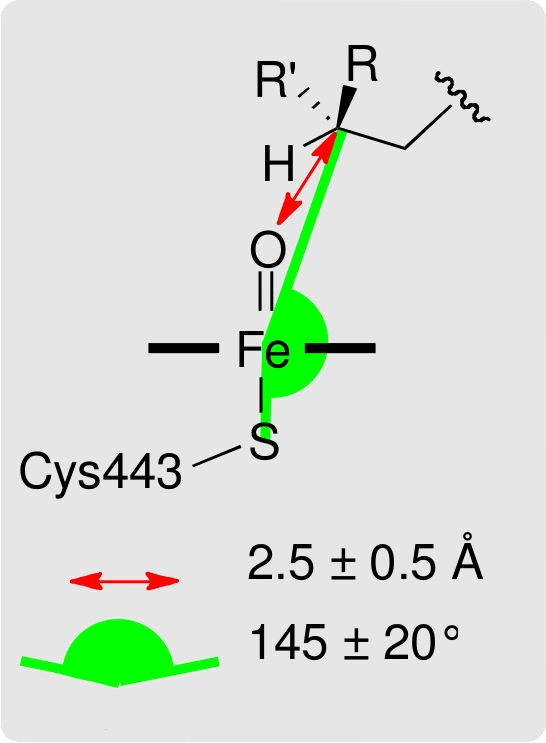
\includegraphics[width=\textwidth]{figures/idsite/33a}
\caption{}
\label{figure:first_sp3_constraints}
\end{subfigure}
\hspace{0.1\textwidth}
\begin{subfigure}[b]{0.35\textwidth}
\centering
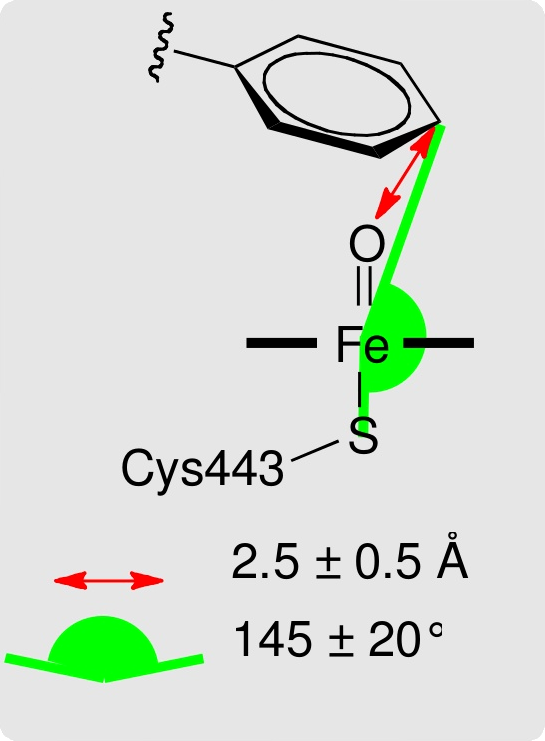
\includegraphics[width=\textwidth]{figures/idsite/33b}
\caption{}
\label{figure:first_sp2_constraints}
\end{subfigure}
\caption{The constraints applied to (a) sp\superscript{3} and (b) sp\superscript{2} atoms during the constrained minimization and first minimization Monte Carlo sampling stage.
The spring constant of the bond constraint (red arrow) is 100 kcal/mol/angstrom\superscript{2}, and that of the angle constraint is 25 kcal/mol/degree\superscript{2}.
The oxygen atom depicted in this figure is a ``dummy'' atom and does not interact with any other atoms in the structure except through the constraint.}
\label{figure:first_constraints}
\end{figure}


In the second minimization Monte Carlo sampling stage, the constraints are different for sp\superscript{2} and sp\superscript{3} carbons.
These constraints are illustrated in figures \ref{figure:second_sp3_constraints} and \ref{figure:second_sp2_constraints}.
For sp\superscript{3} sites:
\begin{enumerate}
\item the hydrogen bound to the carbon at the possible site of metabolism is constrained to a distance of 1.25\plusorminus0.1 angstroms and a spring constant of 20 kcal/mol/angstrom\superscript{2},
\item the carbon in question is constrained to 2.2\plusorminus0.8 angstroms and a spring constant of 10 kcal/mol/angstrom\superscript{2},
\item the heme iron-hydrogen-carbon angle is constrained to 138\plusorminus5 degrees and a spring constant of 20 kcal/mol/degree\superscript{2}.
\end{enumerate}
For sp\superscript{2} sites:
\begin{enumerate}
\item the carbon at the possible site of metabolism is constrained to 1.8\plusorminus0.1 angstroms and a spring constant of 20 kcal/mol/angstrom\superscript{2},
\item both adjacent carbons are also constrained to the dummy oxygen atom, at a distance of 2.5\plusorminus0.1 angstroms and a spring constant of 20 kcal/mol/angstrom\superscript{2}, and
\item finally, the hydrogen bonded to the carbon at the possible site of metabolism is constrained to the oxygen atom at a distance of 2.0\plusorminus0.1 angstroms and a 20 kcal/mol/angstrom\superscript{2} spring constant.
\end{enumerate}
\begin{figure}
    \centering
    \begin{subfigure}[b]{0.35\textwidth}
    \centering
    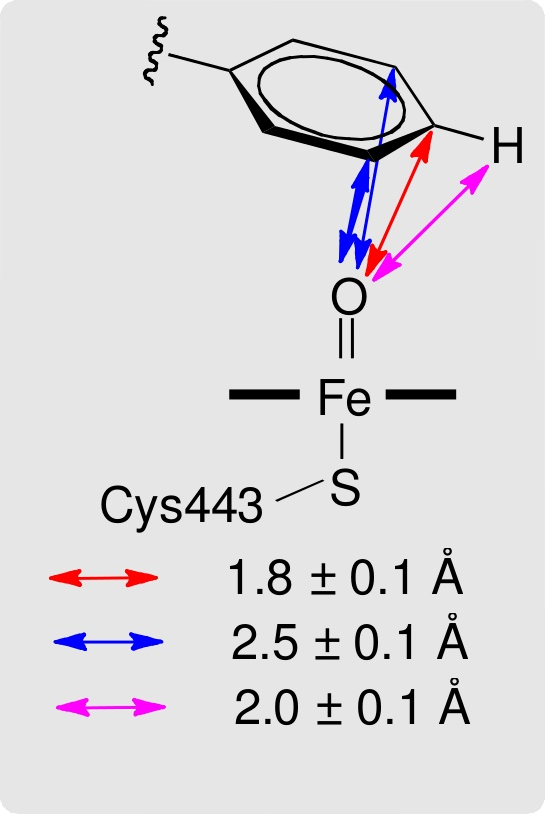
\includegraphics[width=1.0\textwidth]{figures/idsite/34b}
    \caption{}
    \label{figure:second_sp2_constraints}
    \end{subfigure}
    \hspace{0.1\textwidth}
    \begin{subfigure}[b]{0.35\textwidth}
    \centering
    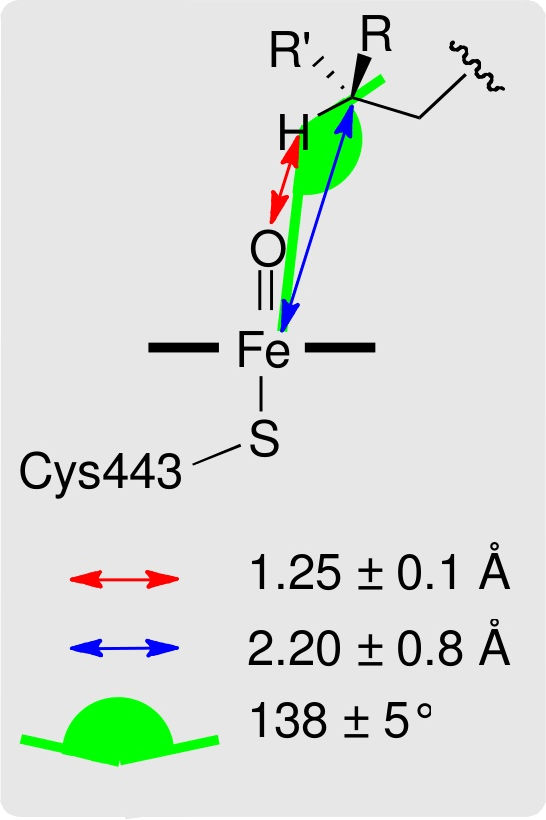
\includegraphics[width=1.0\textwidth]{figures/idsite/34a}
    \caption{}
    \label{figure:second_sp3_constraints}
    \end{subfigure}
    \caption{The constraints applied to (a) sp\superscript{2} and (b) sp\superscript{3} atoms during the constrained minimization and second minimization Monte Carlo sampling stage.}
    \label{figure:second_constraints}
\end{figure}
 

As CYP2D6 forms a conserved salt bridge with the substrate with either glutamate 216 or aspartate 301 \cite{paine2003residues}, this was also incorporated as a constraint during the sampling stages.
In the first sampling stage, this salt bridge is enforced by introducing a harmonic constraint of 3.0\plusorminus0.3 angstroms between the basic nitrogen of the substrate and each of the side chain oxygen atoms in GLU216, ASP301, and SER304 (see figure \ref{figure:salt_bridge_first}).
The spring constants of these constraints are 15.0, 8.0, and 4.0 kcal/mol/angstrom\superscript{2} for GLU216, ASP301, and SER304, respectively.
Additionally, an angle constraint of 150.0\plusorminus30.0 degrees with spring constant of 5.0 kcal/mol/degree\superscript{2} is applied to each of the N-H-O angles.
\begin{figure}[hp]
\centering
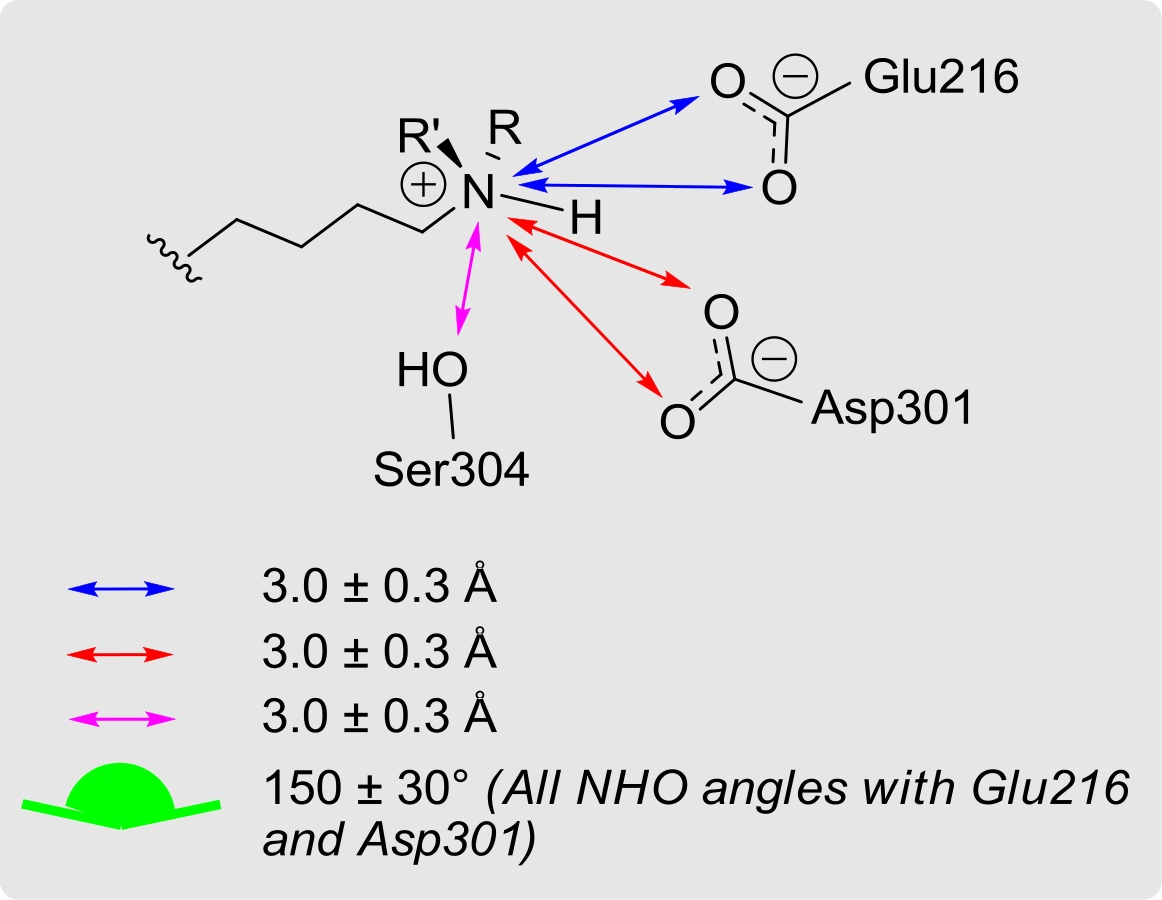
\includegraphics[width=0.50\textwidth]{figures/idsite/salt_bridge_first}
\caption{The constraints applied to the salt bridge region of CYP2D6 during the {\it first} minimization Monte Carlo sampling stage.}
\label{figure:salt_bridge_first}
\end{figure}

In the second sampling stage, four separate trajectories are calculated for each of the four carboxalate oxygens of GLU216, ASP301 (shown in figure \ref{figure:salt_bridge_second}).
In each trajectory a constraint of 1.9\plusorminus0.1 angstroms is applied between the hydrogen attached to the basic substrate nitrogen and one of the four carboxalate oxygens.
Additionally, the angle of the hydrogen bond is constrained to 168\plusorminus12 degrees, with a spring constant of 5.0 kcal/mol/degree\superscript{2}.
\begin{figure}[hp]
\centering
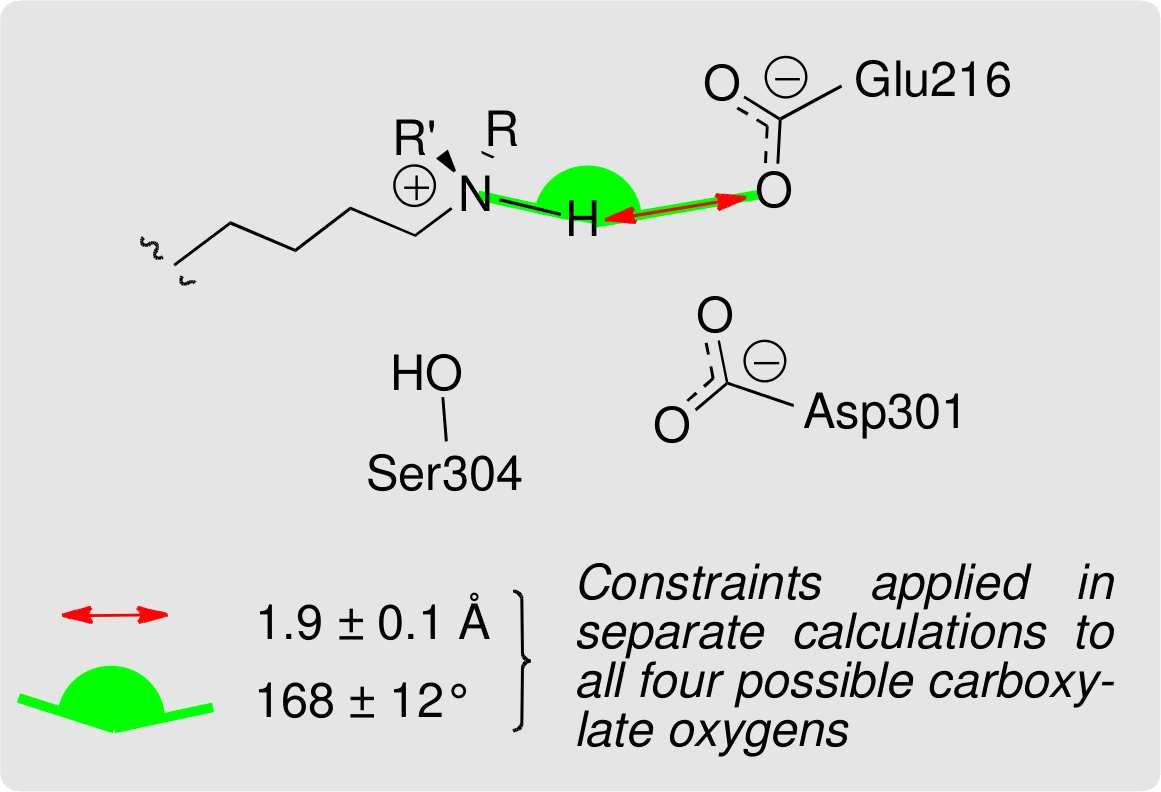
\includegraphics[width=0.50\textwidth]{figures/idsite/salt_bridge_second}
\caption{The constraints applied to the salt bridge region of CYP2D6 during the {\it second} minimization Monte Carlo sampling stage.}
\label{figure:salt_bridge_second}
\end{figure}
 % figure

\begin{figure}[hp]
\centering
\includegraphics[width=0.7\textwidth]{dot_files/mcm_flowchart.png}
\caption{An outline of the Monte Carlo minimization refinement stages in PLOP.}
\label{figure:mcm_flowchart}
\end{figure}

Three different methods of sampling, or moves, were implemented in order to sample different protein-ligand conformations.
A flow chart presenting the minimization Monte Carlo procedure is presented in figure \ref{figure:mcm_flowchart}.
\begin{enumerate}
\item Side chain moves.
Several types of side chain motions were implemented in PLOP.
In all cases, they are defined in a such a way that they can be applied to both ligands and proteins.
The same atomic overlap screening function implemented with the rigid body Monte Carlo was implemented with the side chain torsional moves.
a. Random torsion angle moves: The first type of move that was implemented is random movement of torsional chi angles.
For small torsion moves, a random perturbation of the angle of +/- X is made, where X is a random number with user defined magnitude.
For large torsion moves, for each torsion angle that is changed, a random angle is selected in the form 60*Y +/- X, where Y = 1 through 5, and X is the same random number for the small torsion moves.
The large move was introduced since positions at the top of rotamer barriers are relatively unlikely to be selected, and efficiency thus can be improved by focusing on the more probable moves.
The ratio of small to large torsion moves can be used-adjusted, as can the ratio of probabilities of changing all the torsions in a randomly selected side chain versus changing only one single (randomly selected) torsion among all the free torsions in the simulation can be set as a user-defined parameter.
Rotamer side chain moves: A second type of torsional samples implemented is random selection of a new rotamer state for the entire side chain, plus an optional user defined small noise term for each torsion in the rotamer state.
A database of protein rotamer states obtained from crystallographic data are already a part of PLOP \cite{xiang2001extending} Rotamer libraries for ligands are generated by examining all possible side chain conformations at 10 degree resolution and screening this set for steric clashes.
A Monte Carlo move in this case represents a choice of a new torsional rotamer state for the entire side chain.
Monte Carlo moves based on torsional states cannot lead to correct equilibrium distributions, as transitions from non-rotamer states to rotamer states are defined, but not reverse transitions, upsetting detailed balance.
However, a pretabulated rotamer state is more likely to be low energy than a randomly generated torsional state, and thus allows for more diverse conformational searching.
Correlated torsional moves: Most torsional rearrangements of the side chains in the core of proteins are highly correlated because of the density.
In order to attempt to include correlated torsional motion, at each step we examine the distance between all pairs of beta carbons in the ligands that are free to move.
At each step, for the set of side chains that are free to move, clusters where beta carbons are all mutually within a user-specified distance are identified.
This process takes a trivial amount of time compared to an energy evaluation, so does not slow the simulation at all.
Then, with user specified probabilities, clusters of different sizes are selected for the torsional moves, either with random side chain moves, or rotamer selection moves.
By selecting only clusters where all residues are mutual neighbors, detailed balanced is observed for simulations where accurate equilibrium sampling is desired.
By varying the dihedral angles of the rotatable bonds, IDSite uses side chain MC moves in PLOP to sample the selected side-chain conformations of the protein and of the ligand.
Up to three close residues (C beta distance within 6 angstroms) are allowed to rotate collectively, but the moves of the protein residues and those of the ligand are separated.
In each attempted movement, the conformations of the selected side chains (from the protein/ligand) are either changed by random perturbations or assigned by the randomly selected rotamers from a library.
For an attempt with a random perturbation, the displacement of each dihedral angle is the sum of a large rotation (N times 60 degrees with N as a random integer between 0 and 5) and a random perturbation from 0 to 30 degrees.
For a rotamer library attempt, a side-chain conformation is updated with a random rotamer from a high resolution side-chain library for protein residues \cite{xiang2001extending}, and from a homogeneous library at 10 degree resolution for the ligand.
If a structure with tolerable overlaps is generated in an attempt, it is minimized and sent to subsequent stages for judgment of acceptance.
Each side-chain move takes less than 15 seconds and is the fastest among all the three move types.

% from mike's
For side chain Monte Carlo, a steric screen with an overlap factor of 0.6 was used.
Rotamer torsional moves were selected 75\% of the time, with half of the remaining being of random torsions, and the other half random perturbations of all torsions within the randomly selected side chains.
Clusters of size 1 (i.e. single side chains), size 2 and size three were selected in equal proportion, and all side chains in the cluster were perturbed with the selected torsion move.
A mutual beta carbon distance of 6 Angstroms was used for the clustering size.
Small torsion perturbations made +/- 60 degress from the current dihedral angle, and were performed 5\% of the time; Large periodic moves were performed 95\% of the time.
Only outer steps were performed, and each side chain Monte Carlo series consisted in only one move.
Minimization was performed after the single step, and acceptance was performed at 1 K.


\item % TODO
Rigid motion moves.
Rigid body translation and rotation were also implemented for noncovalently linked moieties, such as ligands.
Random rotations and translations were coupled together, allowing for more concerted movement.
Rigid body move implemented in PLOP can optionally include a screening step, where atomic Lennard-Jones overlaps that would lead to energies much higher than would be observed in any conceivably long equilibrium simulation are rejected without further evaluation.
A ratio of 0.7 between the distance between the two atoms and the sum of the Lennard-Jones radii of the two atoms yields energies on the order of 10's of thousands of kcal/mol, and is thus reasonable to maintain equilibrium sampling in a Monte Carlo simulation.
Translations were implemented in a random direction, with a user-defined magnitude.
Rotations were implemented by picking a random quarternion (a random angle around a random axis, through the geometric center of the rigid group) with a user specified maximum random angle centered around either the current angle, or 180 from the current angle, in the case of a flip.
Multiple time scale Monte Carlo sampling was also implemented with rigid body moves, with short range and long range interactions defined as above.
In addition, an option to compute the inner Monte Carlo loops with reduced Lennard-Jones radii were also implemented, to increase the ability to escape from tight spacial bottlenecks.
In this case, the long time step energies are the full energies with unscaled Lennard-Jones radii.
This increases the conformational freedom and therefore sampling for the short, at a cost of decreasing the acceptance probability in the outer loop.
Scaled Lennard-Jones radii were also implemented in multiple time dynamics, but yielded very little apparent improvement because of the lack of phase space overlap between dynamics with different scaled Lennard-Jones radii).
Rigid body moves are used to sample the translational and rotational space of the ligand.
Multiple attempts with reduced VDW radii are applied, as it is quite common to fail in searching for a clash-free conformation in a single rigid body moving attempt (especially when the ligand is large and flexible and the binding pocket is relatively small).
Each rigid body move includes 1000 attempts, and each attempt performs a translation along a random vector and a rotation around a random axis, with less than 0.5 angstroms and 60 degree displacement, respectively.
In addition, the VDW radii are reduced (scaling factor 0.8) to soften the Lennard-Jones potential, so that mild steric clashes are allowed, which are likely to be resolved by the subsequent minimization.
The rigid body move usually takes 20 to 40 seconds per move.

% from mike's
For rigid body Monte Carlo, a steric screen with an overlap factor of 0.7 was used, with a translation size of 0.5 Angstroms and a rotation size of plus or minus 60 degrees.
No flip moves were included, as flips were not anticipated with the geometry of the ligand system [Robert, check this is true?] A Lennard-Jones scaling parameter of 0.8 was used during the inner steps.
Each rigid MC step consisted of 1000 inner steps, and only one outer step, meaning that only one minimization occurred each time rigid body Monte Carlo was selected as the move step.


\item The Hybrid Monte Carlo (HMC) \cite{duane1987hybrid} step is a velocity verlet molecular dynamics simulation.
This simulation allows all atoms in both the ligand and residues containing atoms withing 5 angstroms of the ligand to move.
Initial velocities are taken from a Maxwell-Boltzmann distribution at 900 K.
Bonded and short range interactions evaluated every 1 nanosecond inner time step, and long range potentials are assumed to be fixed over inner steps.
Five inner steps compose each outer HMC step.
In the outer step the molecular surface, long range interactions and, Born alphas are updated before computing the energy and applying the Metropolis acceptance criteria at a temperature of 900 K after each MD run.
Taking up to 15 minutes per move, the HMC is the most expensive among all three types of moves in PLOP.

%, with long range interactions evaluated every long time step.
%In this case, molecular dynamics is run only using only the short range energies, which will conserve energy and thus yield proper Markov chain behavior while the cutoffs and Born alpha are not updated.
%Inner loop Monte Carlo steps are performed with only the short range dynamics, and outer loop Monte Carlo steps are performed with all interactions.
%In the case of implicit solvent simulations, the Born alpha are only reevaluated in the outer loop Monte Carlo steps.
%This allows for evaluation of the full surface integral relatively infrequently, and yields a properly weighted Boltzmann distribution of conformations without needing position derivatives of the Born alphas.

%Energies are conserved in vacuum simulations if the long range cutoff extends to cover the entire molecule.
%With implicit solvent dynamics, energies are not conserved as there is no derivative of the Born alpha with respect to position, so a thermostat must be used to approximate realistic dynamics.
%One mode of action is to run HMC on top of normal RESPA dynamics, with acceptance and rejections done after a fixed number of steps of MD, as in typical HMC.
%Velocities are re-randomized after every Monte Carlo step from the Maxwell-Boltzmann distribution.
%However, HMC can also be implemented in a multiple-time step Monte Carlo framework \cite{hetenyi2002multiple}.
%The hybrid Monte Carlo (HMC)\cite{duane1987hybrid} move in PLOP performs simultaneous sampling for the selected residues in the protein side chains and backbone as well as the ligand.
%Each HMC move performs a 5 picosecond, constant energy molecular dynamic (MD) simulation (starting at 900K) on all the atoms in the selected residues.
%Taking up to 15 minutes per move, the HMC is the most expensive among all three types of moves in PLOP.

%The underlying molecular dynamics for the hybrid Monte Carlo consisted of 500 5 ns RESPA \cite{tuckerman1991molecular} steps, each with 5 1 ns short range steps.
%The dynamics were initialized from a Maxwell-Boltzmann distribution at 900 K, and then run without any thermostat the full 2.5 ps run.
%Minimization was performed after the single HMC step, with acceptance/rejection performed at a Monte Carlo temperature of 900 K.

% is built on top of a molecular dynamics (MD) integrator.
% We implemented velocity verlet MD using the RESPA formalism \cite{tuckerman1991molecular}, with bonded and short range interactions evaluated every inner time step, with long range interactions evaluated every long time step.
% We also included in the including Andersen, Berendsen, and Langevin thermostats, as well as Brownian Dynamics.
% Short range interactions included all bonded interactions and nonbonded interactions less than a user-specified cutoff.
% Both short and long range cutoffs are dipole-based as described in a previous paper [cite].
% and then run without any thermostat the full 2.5 ps run.

\end{enumerate}

\subsection{Evaluation}
\label{subsection:p450/evaluation}
Both a parameterized and an unparameterized model were used to classify potential sites of metabolism.
IDSite makes the assumptions that all intermediates before the rate determining step are at equilibrium \cite{wang2007stochastic}, that hydrogen abstraction is the rate limiting step for hydroxilation of aliphatic carbons and electrophilic attack is the rate limiting step for hydroxilation of aromatic rings \cite{guengerich2001common,shaik2005theoretical}.
With these assumptions the rate of metabolism at each possible site of reaction is affected by the free energy of binding in order to put that site in the site of reaction, as well as the free energy barrier of rate determining step, or
\input{equations/curtin_hammett} % dG = dG bind + dG react
The ${\Delta}G_{\mathrm{binding}}$ above is calculated using a PLOP evaluation of the refined pose.
The intrinsic reactivity for the system is computed from DFT calculations on a simplified system, replacing the heme with a methody radical, and using a linear relationship between $IR(\mathrm{heme})$ and $IR(\mathrm{methoxy\ radical})$ to estimate the true reactivity for the heme system.
\begin{figure}[h]
\centering
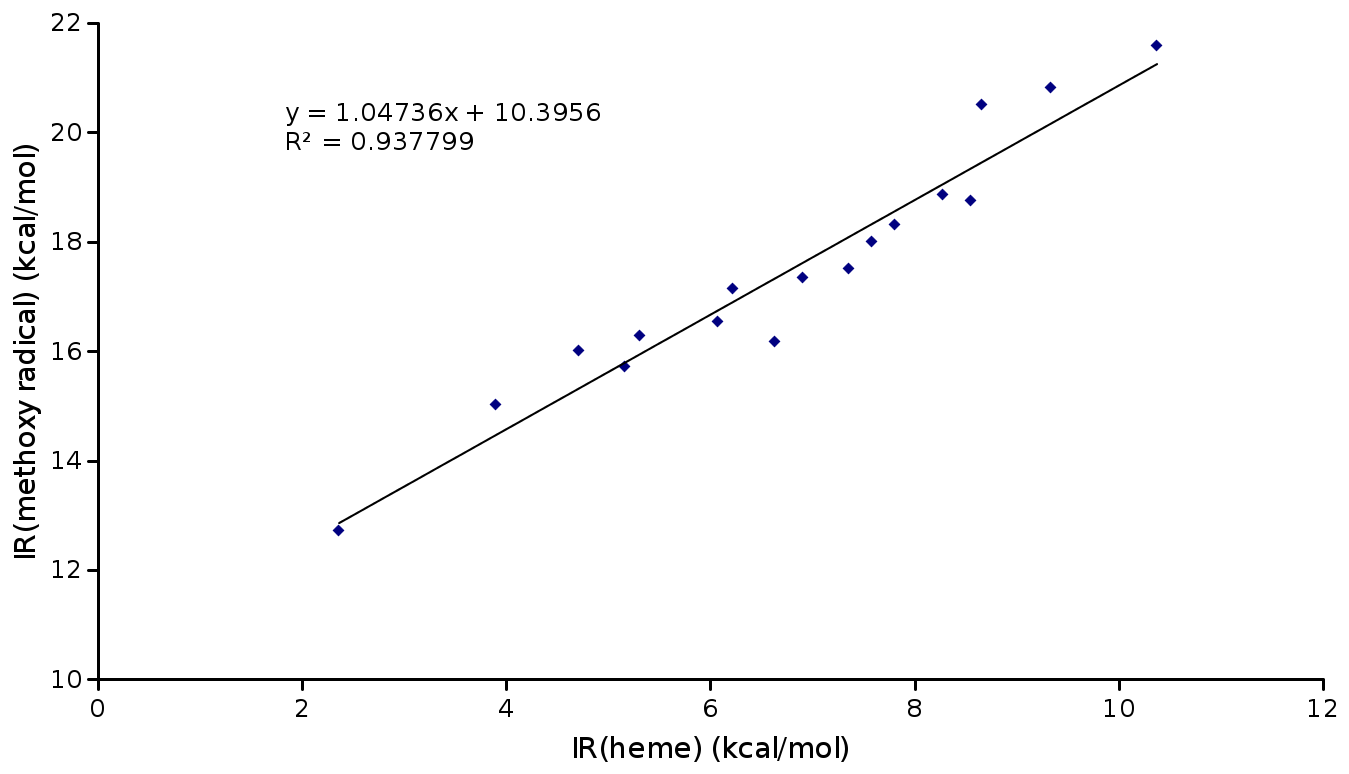
\includegraphics[width=0.8\textwidth]{figures/idsite/intrinsic_corrected.png}
\label{fig:idsite/intrinsic}
\caption{The linear relationship between the calculated intrinsic reactivity of the methoxy radical complex and that of the heme complex.
Adapted from \protect\cite{li2011idsite} with minor correction.
In the original manuscript the slope of the regression was reported as 1.117 and that number was used throughout.
This difference should not significantly affect the physical IDSite classifier results, and does not affect the results of the fit model.
In the rest of this text the value from the original publication of 1.117 will be used.}
\end{figure}
\input{tables/heme_methoxy.tex}
\input{equations/intrinsic_reactivity} % estimate from abbreviated reactivity
Since this constant $C$ is identical for each state it has no effect on the relative differences in ${\Delta}G_{\mathrm{site}}$ or the relative rate of metabolism at possible sites.
\input{equations/g_site} % E/G equation
Since the ligand is forced to assume a different conformation in order to react, the energy of this transition state conformation, $E_{\mathrm{TS}}$, is also computed using PLOP.
As the relative abundance of different metabolites is determined by differences in ${\Delta}G$ per site rather than absolute reactivities, the constant in equation \ref{equation:g_site} does not affect which metabolites are produced.
A site of possible metabolism is classified as positive if it is observed in greater than 0.1\% yield, which corresponds to a \ddg\ of \textapprox4.75 kcal/mol between the most favored state and the cutoff for negative predictions. 

The second classifier is similar however:
\begin{enumerate}
\item a different constant is used to estimate $IR(\mathrm{heme})$ from $IR(\mathrm{methoxy\ radical})$, namely 1.071,
\item if the binding energy of the transition state complex of a pose is within 5.26 kcal/mol of the lowest pose, it is set to the binding energy of the lowest pose.
Otherwise the difference is scaled by 0.58,
\item and the cutoff for an active prediction is changed from 4.75 kcal/mol to 1.46 kcal/mol.
\end{enumerate}
These parameters were decided upon by maximizing $\frac{\mathrm{true\ positives}}{(\mathrm{false\ positives + false\ negatives})}$ on a training set of 36 compounds.


\section{Results}
\label{section:p450/results}
Both physical and fitted IDSite were able to acheive promising results predicting CYP2D6 sites of metabolism.

The physical model correctly identified 68 of 82 active sites of metabolism for a sensitivity of 0.829.
For inactive sites this model correctly identified 1054 of 1075 inactive sites with a specificity of 0.980.
The fit model performed similarly, and even slighly better identifying 52 of 57 sites of metabolism (sensitivity of 0.912) in the training set and 25 of 25 in the test set (sensitivity of 1.0).
\begin{equation}
\mathrm{sensitivity} = \frac{TN}{TN + FP} = \frac{\text{\# of true sites of non-metabolism identified}}{\text{\#\ experimental\ sites\ of\ non-metabolism}}
\end{equation}

\begin{equation}
\mathrm{sensitivity} = \frac{TP}{TP + FN} = \frac{\text{\#\ of\ true\ sites\ of\ metabolism\ identified}}{\text{\#\ experimental\ sites\ of\ metabolism}}
\end{equation}

\begin{table}[h]
\singlespace
\footnotesize
\centering
\begin{tabular}{cccccccccc}
\hline
	&	&Physical	&	&	&Fitted	&	&	&	&\\
Compound \#	&Compound Name	&TP	&FP	&FN	&TP	&FP	&FN	&	&\\
\hline
1	&4-methoxyamphetamine	&1	&0	&0	&1	&0	&0	&	&\\
2	&Amitriptyline	&2	&2	&0	&2	&0	&0	&	&\\
3	&Aprindine	&4	&0	&1	&5	&0	&0	&	&\\
4	&Brofaromine	&1	&0	&0	&1	&0	&0	&	&\\
5	&Bufuralol	&0	&1	&1	&1	&0	&0	&	&\\
6	&Carvedilol	&1	&0	&2	&2	&0	&1	&	&\\
7	&Cinnarizine	&0	&2	&1	&0	&2	&1	&	&\\
8	&Clomipramine	&1	&0	&1	&1	&0	&1	&	&\\
9	&Codeine	&1	&0	&0	&1	&0	&0	&	&\\
10	&Desipramine	&2	&0	&0	&2	&0	&0	&	&\\
11	&Dextromethorphan	&1	&0	&0	&1	&0	&0	&	&\\
12	&Dihydrocodeine	&1	&1	&0	&1	&0	&0	&	&\\
13	&Ethylmorphine	&1	&0	&0	&1	&0	&0	&	&\\
14	&Flunarizine	&1	&0	&0	&1	&0	&0	&	&\\
15	&Fluperlapine	&1	&0	&0	&1	&0	&0	&	&\\
16	&Hydrocodone	&1	&0	&0	&1	&0	&0	&	&\\
17	&Imipramine	&2	&0	&0	&2	&0	&0	&	&\\
18	&Indoramine	&1	&0	&0	&1	&0	&0	&	&\\
19	&MDMA	&1	&0	&0	&1	&0	&0	&	&\\
20	&Methamphetamine	&1	&0	&0	&1	&2	&0	&	&\\
21	&Methoxyphenamine	&2	&0	&0	&2	&0	&0	&	&\\
22	&Metoprolol	&1	&0	&1	&2	&0	&0	&	&\\
23	&Mexiletine	&2	&0	&1	&2	&0	&1	&	&\\
24	&Mianserin	&1	&0	&0	&1	&0	&0	&	&\\
25	&Mirtazapine	&0	&1	&1	&1	&1	&0	&	&\\
26	&Nortriptyline	&1	&1	&0	&1	&0	&0	&	&\\
27	&Ondansetron	&2	&0	&0	&1	&0	&1	&	&\\
28	&Paroxetine	&1	&0	&0	&1	&0	&0	&	&\\
29	&Perhexiline	&2	&0	&0	&2	&0	&0	&	&\\
30	&Propafenone	&1	&1	&0	&1	&1	&0	&	&\\
31	&Propranolol	&2	&2	&0	&2	&1	&0	&	&\\
32	&Tamoxifen	&1	&0	&0	&1	&0	&0	&	&\\
33	&Terfenadine	&3	&0	&0	&3	&0	&0	&	&\\
34	&Tiracizine	&1	&2	&0	&1	&1	&0	&	&\\
35	&Tropisetron	&2	&0	&1	&3	&0	&0	&	&\\
36	&Venlafaxine	&1	&0	&0	&1	&0	&0	&	&\\
	&TOTAL	&47	&13	&10	&52	&8	&5	&	&\\
\hline
\end{tabular}
\caption{Results of physical and fitted IDSITE on training set of 36 compounds.}
\label{table:p450_training}
\end{table}

\begin{table}[h]
\singlespace
\footnotesize
\centering
\begin{tabular}{cccccccc}
\hline
 &  &  & Physical &  &  & Fitted & \\
Compound \# & Compound & TP & FP & FN & TP & FP & FN \\
\hline
37 & Atomoxetine & 0 & 1 & 1 & 1 & 2 & 0 \\
38 & Bicifadine & 1 & 2 & 0 & 1 & 0 & 0 \\
39 & Bupranolol & 1 & 0 & 0 & 1 & 0 & 0 \\
40 & Carteolol & 1 & 1 & 0 & 1 & 0 & 0 \\
41 & Chlorpromazine & 1 & 0 & 0 & 1 & 0 & 0 \\
42 & EMAMC & 1 & 0 & 0 & 1 & 0 & 0 \\
43 & Encainide & 1 & 1 & 0 & 1 & 1 & 0 \\
44 & Harmaline & 1 & 0 & 0 & 1 & 0 & 0 \\
45 & Harmine & 1 & 1 & 0 & 1 & 1 & 0 \\
46 & Ibogaine & 1 & 0 & 0 & 1 & 0 & 0 \\
47 & MAMC & 1 & 0 & 0 & 1 & 0 & 0 \\
48 & MMAMC & 1 & 0 & 0 & 1 & 0 & 0 \\
49 & MOPPP & 1 & 0 & 0 & 1 & 0 & 0 \\
50 & Oxycodone & 1 & 0 & 0 & 1 & 0 & 0 \\
51 & Spirosulfonamide & 2 & 0 & 0 & 2 & 0 & 0 \\
52 & Timolol & 2 & 0 & 2 & 4 & 0 & 0 \\
53 & Tolterodine & 0 & 1 & 1 & 1 & 1 & 0 \\
54 & Tramadol & 1 & 1 & 0 & 1 & 1 & 0 \\
55 & Tyramine & 2 & 0 & 0 & 2 & 0 & 0 \\
56 & Zotepine & 1 & 0 & 0 & 1 & 0 & 0 \\
 & Total & 21 & 8 & 4 & 25 & 6 & 0 \\
\hline
\end{tabular}
\caption{Results of physical and fitted IDSite on a test set of 20 compounds.
Note that for the physical model there is no training performed so results in the text are presented in a unified fashion for the training and test set.}
\label{table:p450_testing}
\end{table}






The fit model also correctly identified 709 of 717 inactive sites in the training set (specificity of 0.989) and 352 of 358 inactive sites in the test set (specificity of 0.983).
As the performance of the fit model is similar to that of the physical model, it does not appear that the fit model is overparameterized to the training set.
Specific results for both models are presented in Tables \ref{table:p450_training} and \ref{table:p450_testing}, and the specific sites identified by both models as well as experiments are illustrated in Figures \ref{fig:idsite_traininga} and \ref{fig:idsite_test}. 

We believe that the parameters help account for some degree of noise in the molecular mechanics calculations.
The scaling of the binding energy difference, either to zero inside a window about the minimum energy pose, or by a factor of 0.58 decreases the relative weight of the molecular mechanics contribution relative the quantum contribution to the classifier.
This might imply that some sites are not being classified as active because they are not in the lowest energy conformation around the docked pose, suggesting that additional molecular mechanics sampling might further improve results.
However as will be discussed later, the molecular mechanics stage already dominates the total time necessary for an IDSite prediction, and the current molecular mechanics procedure takes about 450 hours.   

\begin{figure}
\centering
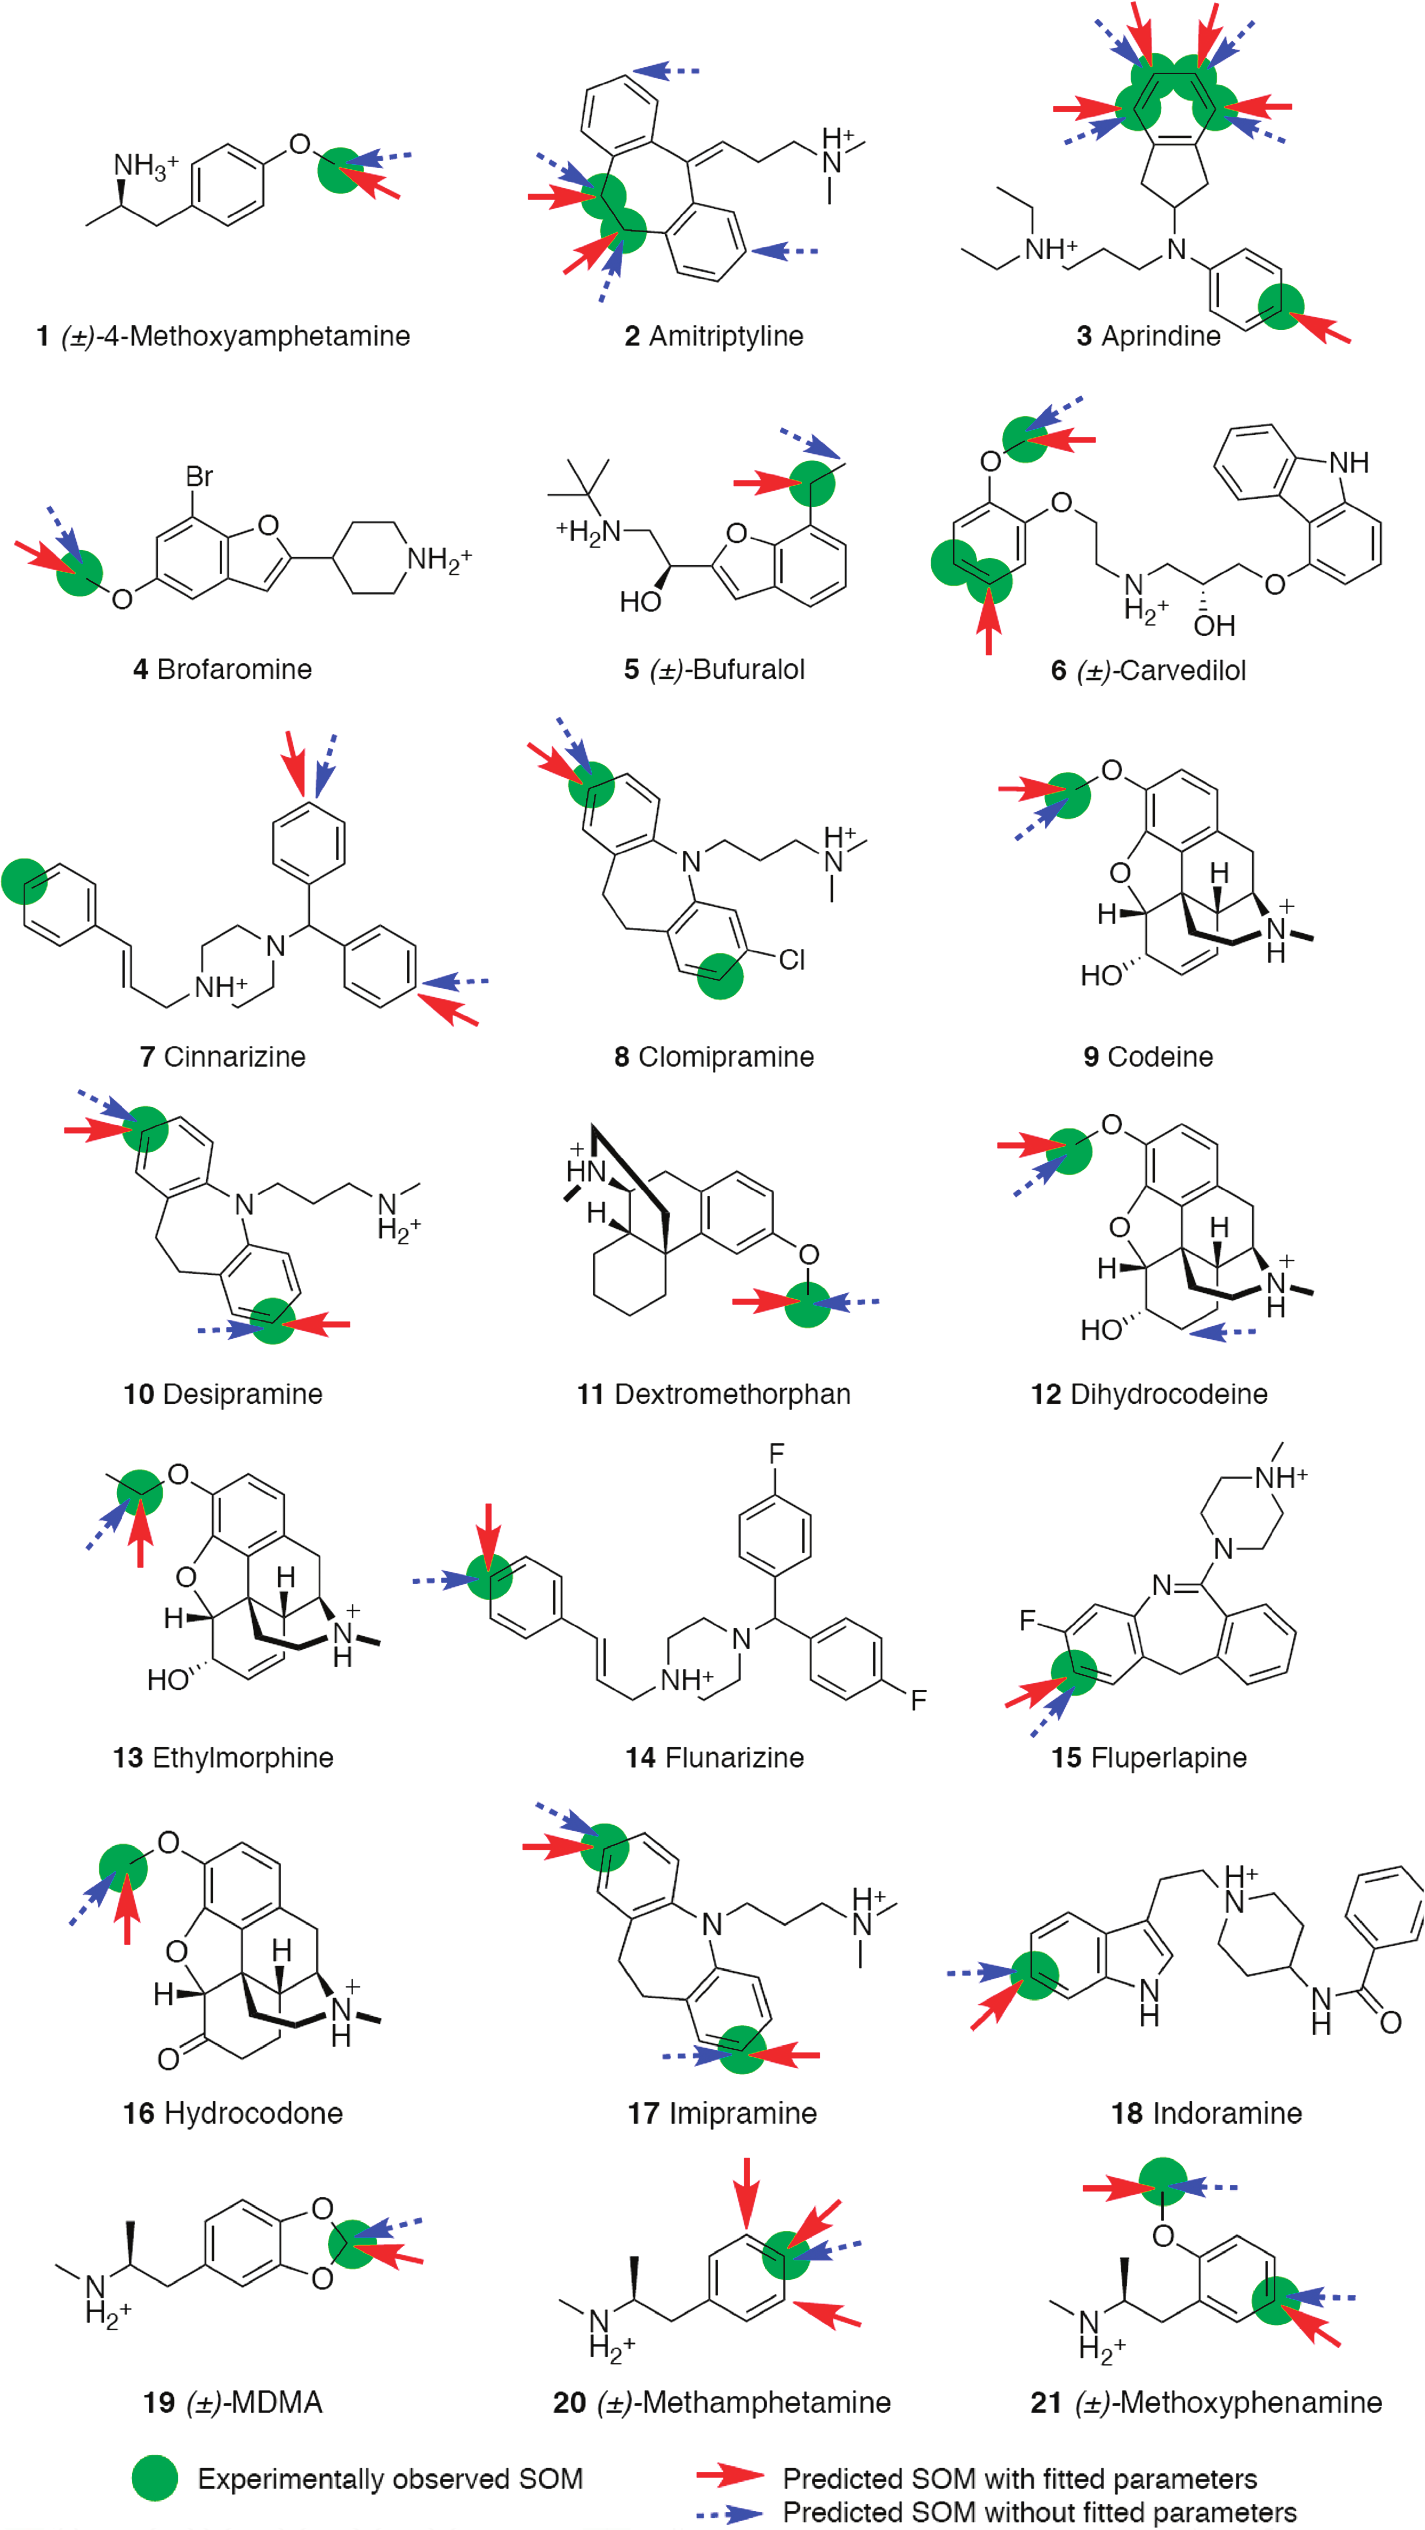
\includegraphics[width=0.65\textwidth]{figures/idsite/idsite_figure-007.png}
\caption{Physical and fitted IDSite predictions of sites of metabolism on the training set.}
\label{fig:idsite_traininga}
\end{figure}

\begin{figure}
\ContinuedFloat
\centering
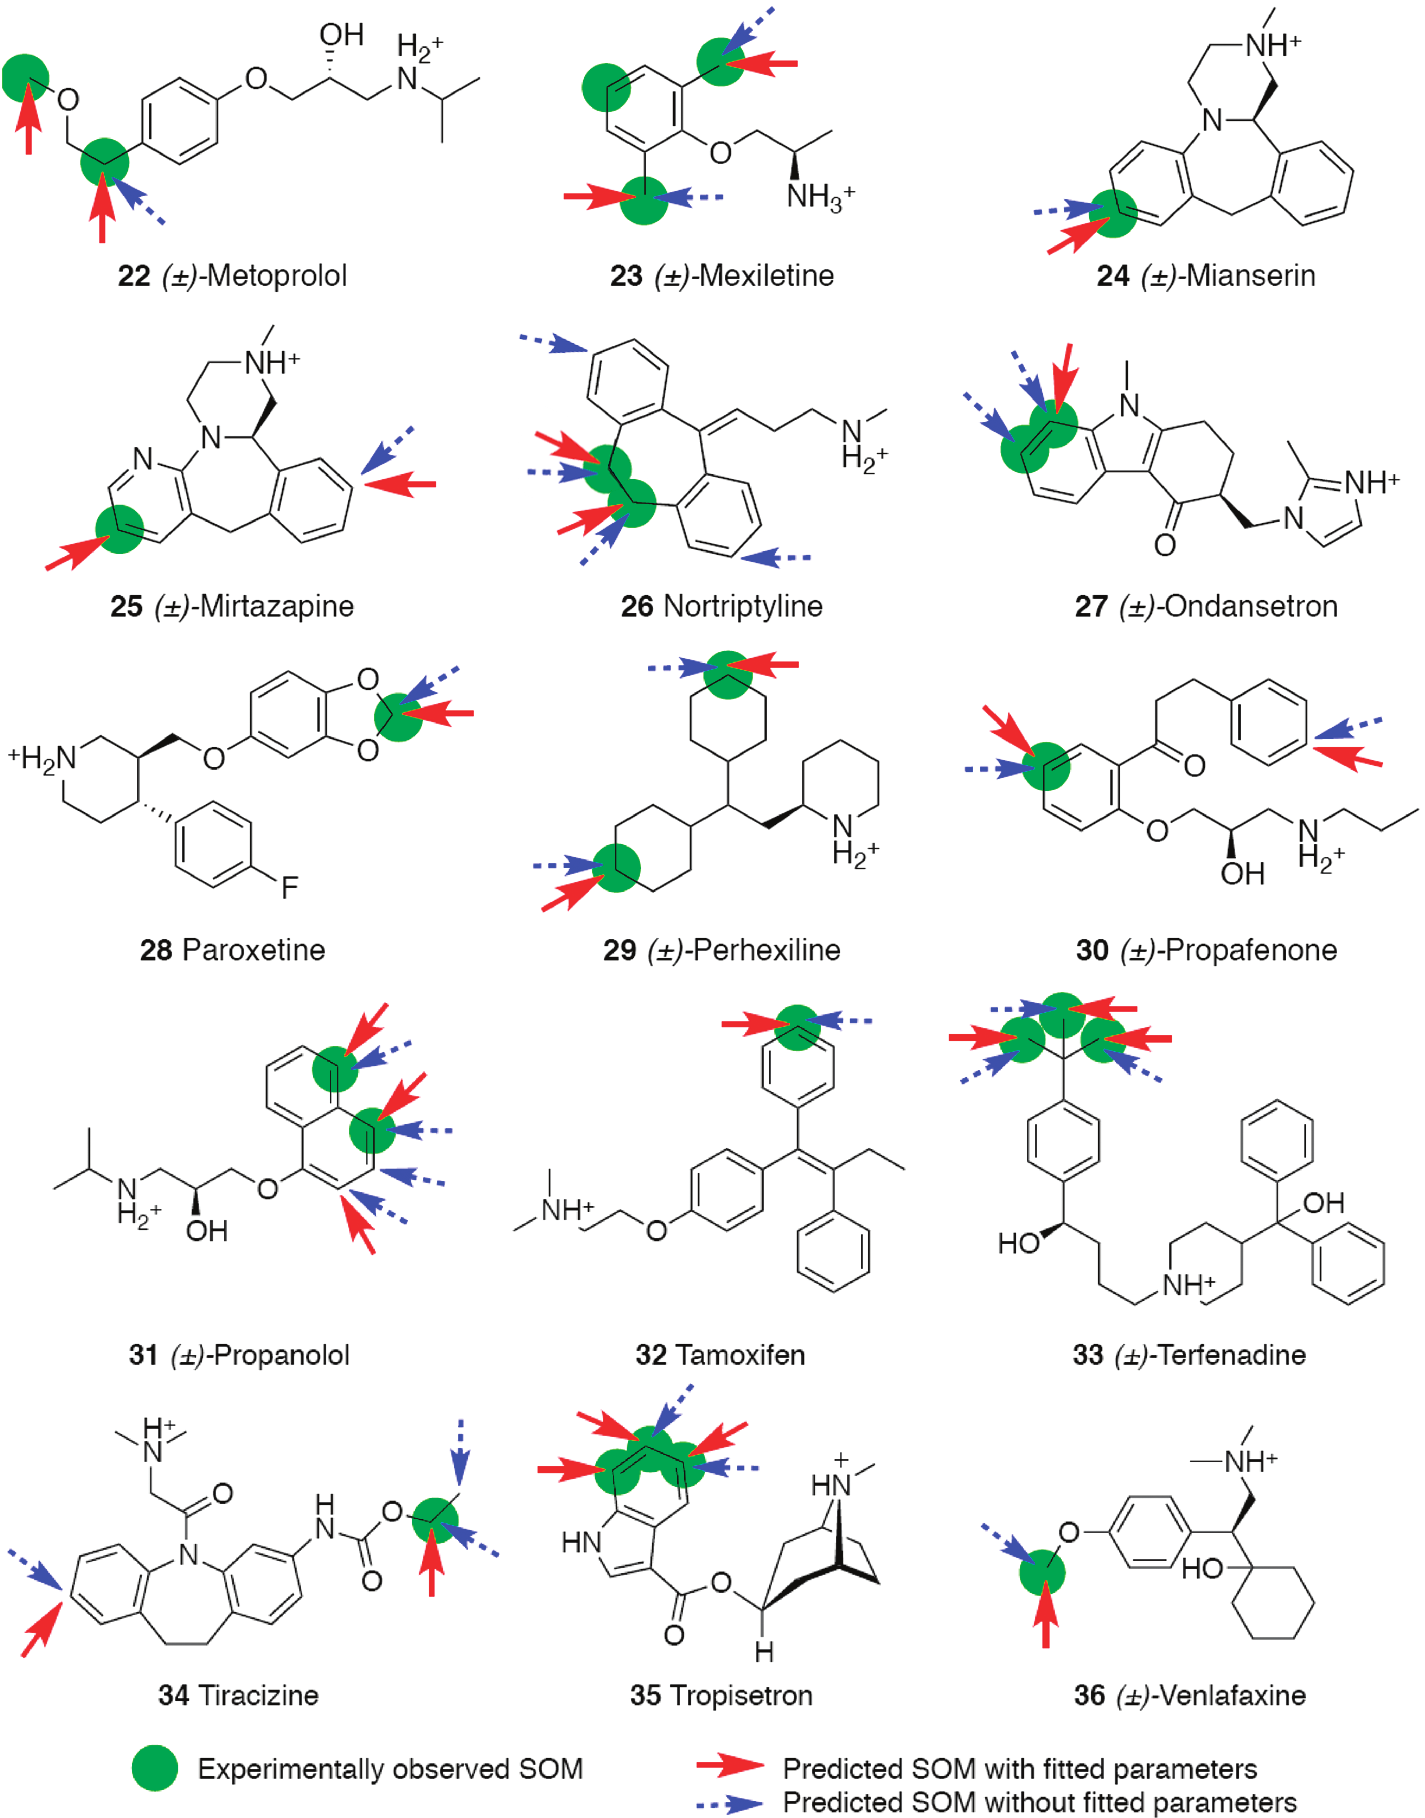
\includegraphics[width=0.65\textwidth]{figures/idsite/idsite_figure-008.png}
\caption{(continued)}
\label{fig:idsite_trainingb}
\end{figure}


\begin{figure}
\centering
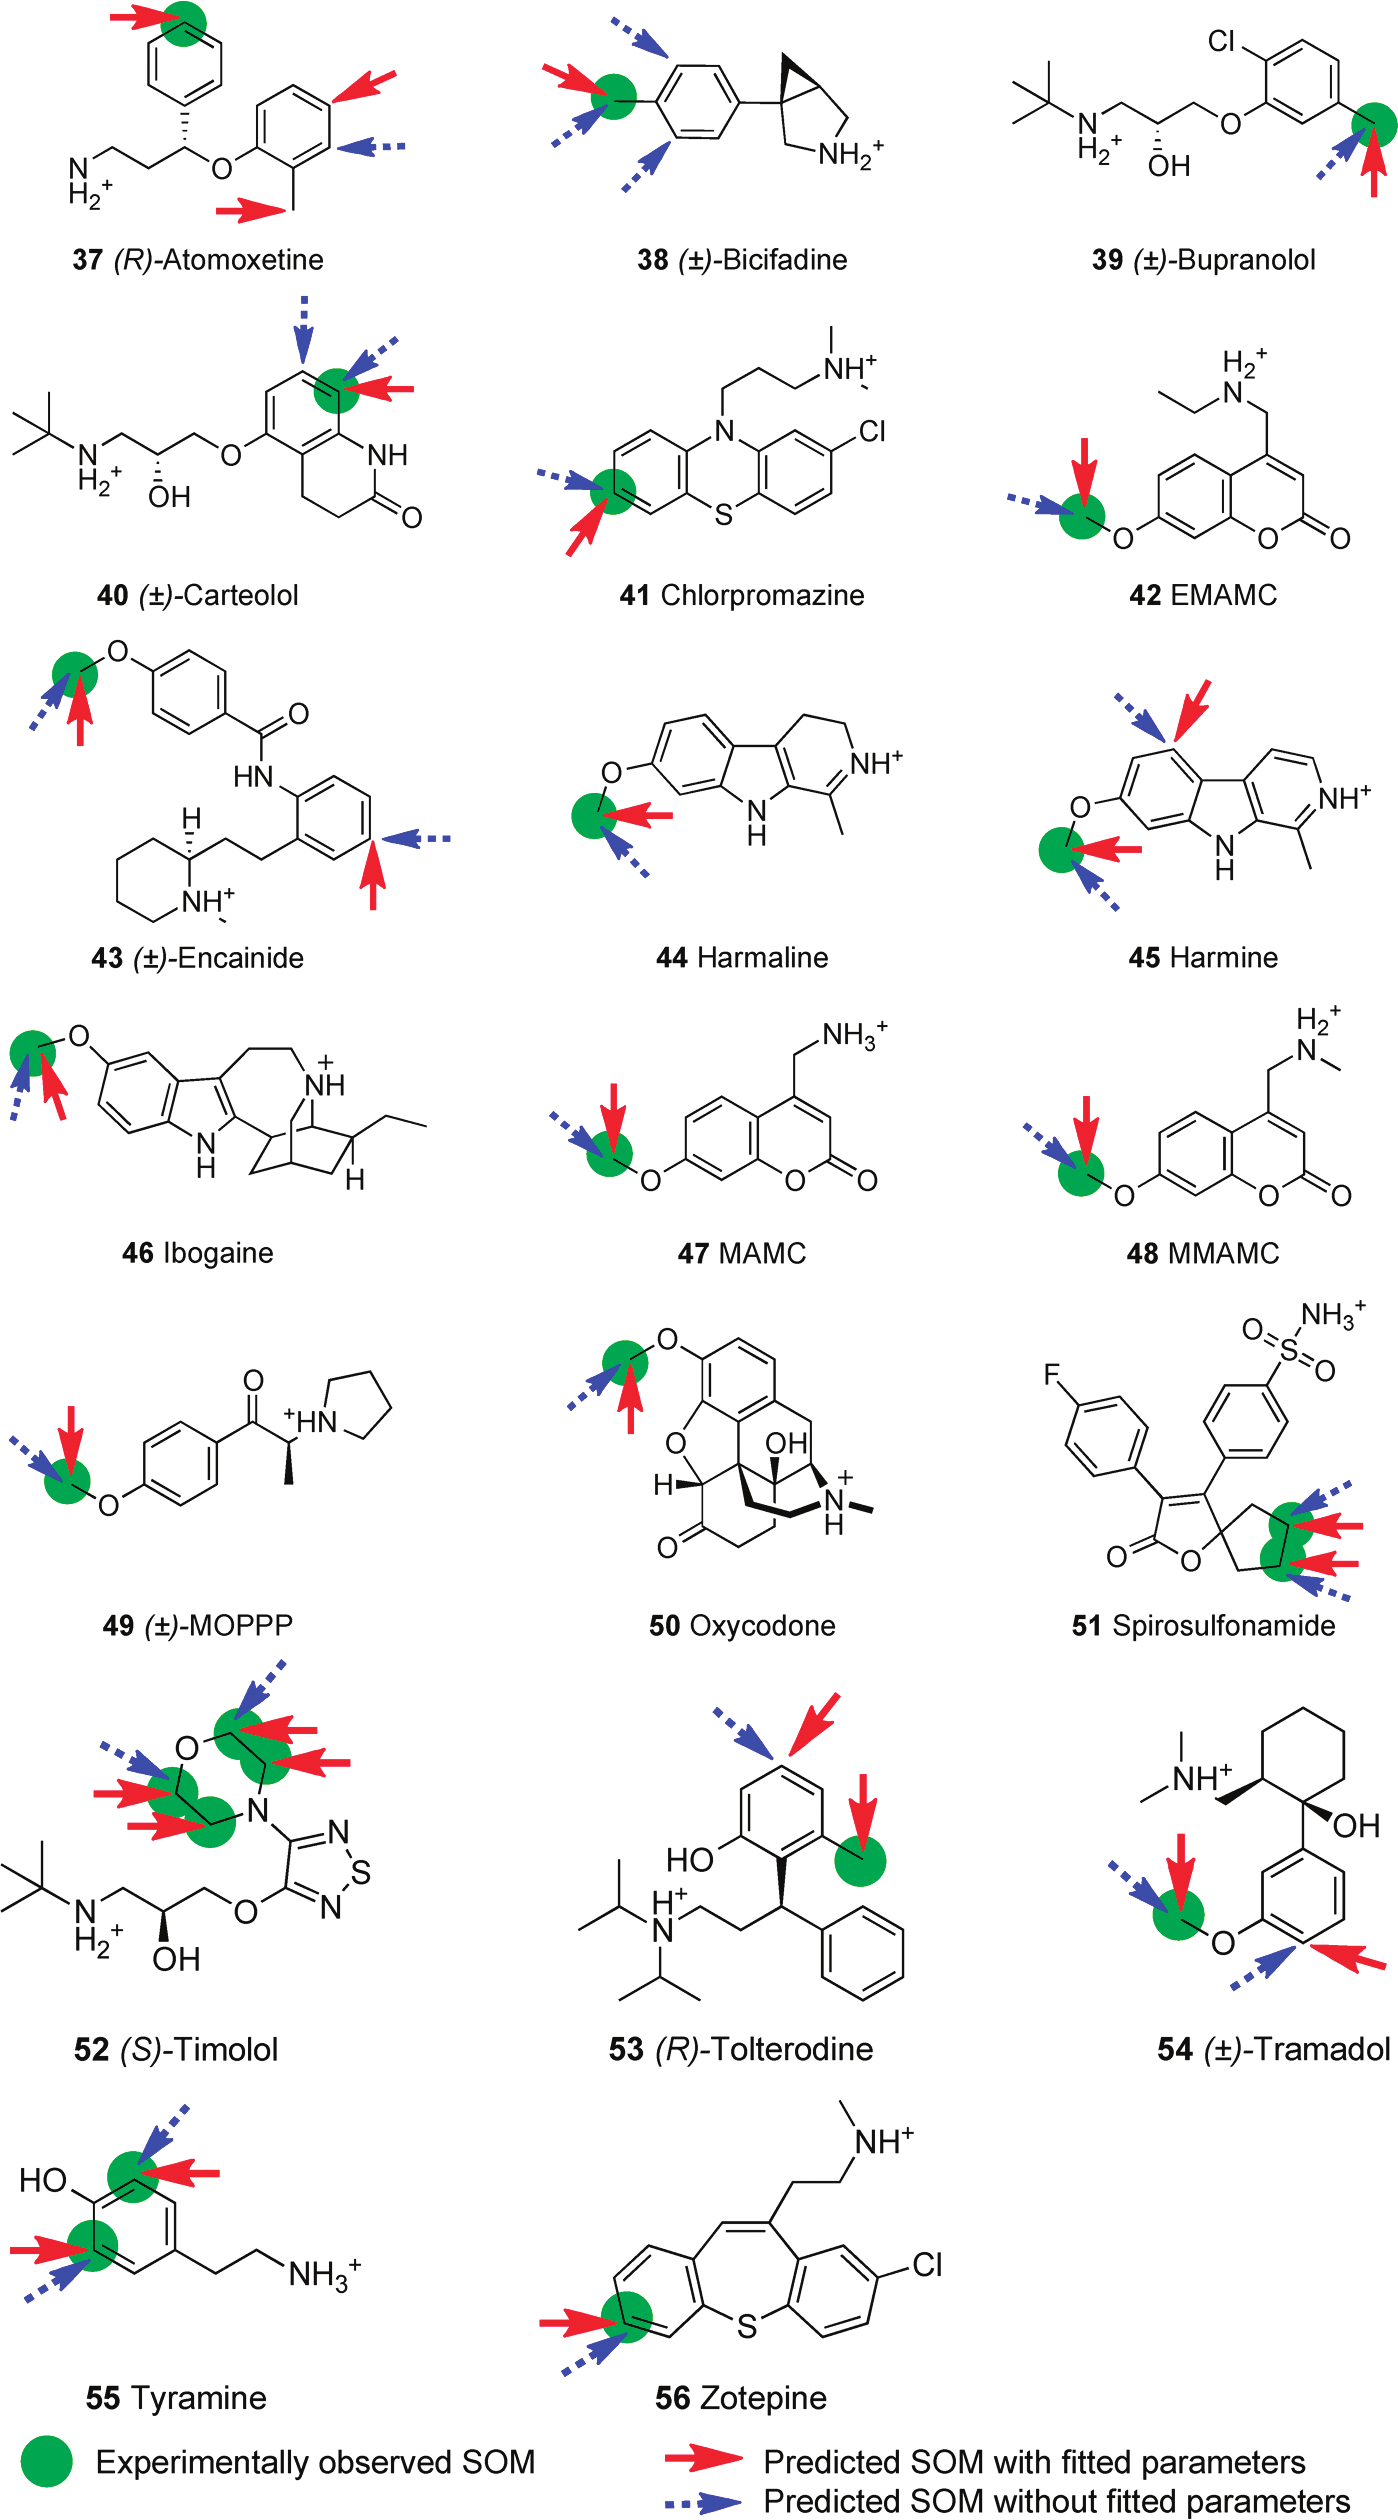
\includegraphics[width=0.65\textwidth]{figures/idsite/idsite_figure-009.png}
\caption{Physical and fitted IDSite predictions of sites of metabolism on the test set.}
\label{fig:idsite_test}
\end{figure}


\section{Discussion}
\label{section:p450/discussion}


%\chapter[p450 Sites of Metabolism]{Prediction of p450 Sites of Metabolism}
\section{Introduction}
\label{section:p450/introduction}
The most common method of drug clearance among currently perscribed drugs is metabolism, which is the primary method of clearance for approximately 75\% of the top 200 most commonly perscribed drugs in the United States \cite{williams2004drug}.
Cytochrome p450 is critical to drug metabolism, being active in approximately 75\% of drugs which are cleared in this method \cite{guengerich2007cytochrome}.

\begin{figure}[h]
\centering
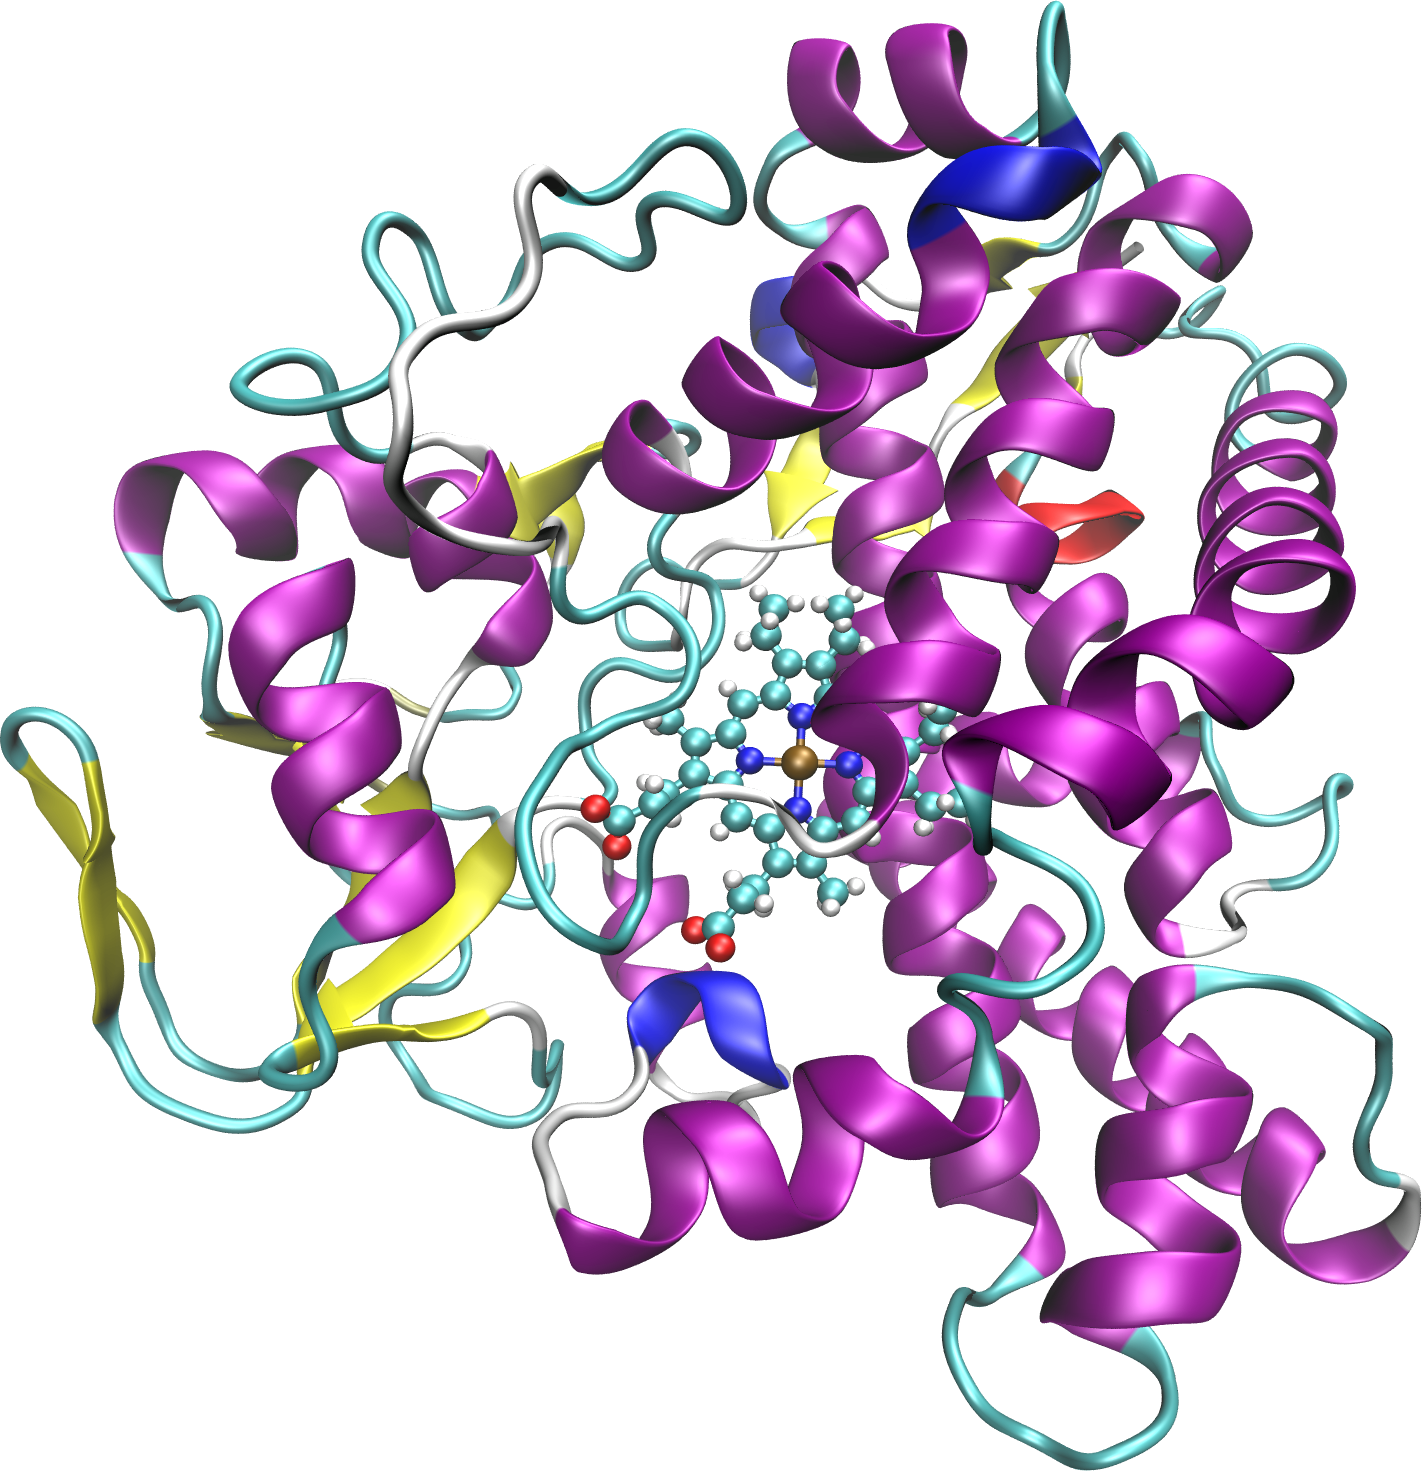
\includegraphics[width=0.5\textwidth]{figures/p450.png}
\caption{
The structure of cytochrome P450, taken from PDBid 1JFB, shown in cartoon representation.
The bonded heme group, shown as ball and stick model, is visible in the center.
}
\label{fig:p450}
\end{figure}


\section{Methods}
\label{section:p450/methods}

\begin{figure}[h!]
\centering
\includegraphics[width=0.55\textwidth]{dot_files/idsite.png}
\caption{An overview of the entire IDSite procedure.
The dotted lines represent abbreviated versions of the full procedure.
Receiver operating characteristic graphs for the full version, and these abbreviated versions, are presented in \ref{figure:idsite_roc_sampling}.
Series colors on ROC graphs correspond to arrow colors here.}
\label{figure:idsite_overview}
\end{figure}

Prediction of sites of metabolism is a three stage procedure:
\begin{enumerate}
\item Initially a number of different ligand conformations are generated, and these are docked into a rigid protein, with soft VDW terms using Glide \cite{halgren2004glide,friesner2004glide}.
\item The docked conformations are refined using a Monte Carlo Minimization (MMC) approach which samples degrees of freedom in both the ligand and protein.
\item Refined conformations are classified into reactive site or non-reactive site on the basis of the energy of the refined conformations and the intrinsic reactivity of the site. \cite{li2011idsite}
\end{enumerate}

\subsection{Docking}
\label{subsection:p450/docking}
In the initial docking stage of the IDSite protocol Glide is used to generate a number of proposed docked conformations for each ligand.
Glide (standard precision) is used to generate a number of different ligand conformations by sampling conformations of freely rotatable bonds and rings.
A bounding box, which will be used for a grid search, is defined centered at the centroid of the ligand with an edge length of 10 angstroms.
Because the crystal structure used for CYP2D6 (PDBID: 2F9Q) does not have a ligand, the centroid of residues Glu216, Asp301, Thr309, and Phe483 was used instead in this case.
Because the steric clashes present in many proposed docked conformations can be relieved using a simple minimization procedure a reduced Van der Waals (VDW) radii are used in the docking stage for non-polar atoms.
The VDW radii used for the P450 are scaled by a factor of 0.4, and the scaling for the ligand starts at 0.8.
If an insufficient number of poses, in this case fewer than four, are found using these scaling factors for the radii the scaling of the ligand is stepped down until at least four poses are found.
Additional filtering of possible high energy conformations was also skipped in order to ensure the greatest diversity of docked poses reached the refinement stage.
The collection of docked poses are then clustered according to the RMSD of the ligand, and each pose is minimized.
The top sixty ranked poses according to the Glide SP metric are retained screened using a number of different criteria.
A hard sphere overlap criteria is used to remove poses with obvious steric clashes which were not removed during the minimization procedure.
A conserved feature of CYP2D6 ligand complexes is a salt bridge with Glu216 or Asp301.
In order to reduce sampling cost IDSite only considers structures with at least one hydrogen-bond donor within 4 residues of the centroid of these two residues and Ser304.
The sphere defined by these residues is illustrated along with the bounding box used for sampling in Figure \ref{fig:idsite_glide}
A number of other rule based geometric screens are used to remove structures which are unlikely to react.
Structures meeting any of the following criteria:
\begin{enumerate}
\item The distance of the basic nitrogen to the ferryl oxygen is less than 5.0 angstroms;
\item The distance of the basic nitrogen to the negative charged oxygen (in Glu216 or Asp301) is greater than 5.5 angstroms;
\item More than 2 heavy atoms from the ligands are further than 16.0 angstroms away from the heme iron;
\item More than 1 heavy atom from the ligand are closer than 1.0 angstroms to the receptor;
\item More than 6 heavy atoms from the ligand are closer than 1.8 angstroms to the receptor;
\item No heavy atom in the ligand is within 5.0 angstroms to the heme iron;
\end{enumerate}
are removed.
If the number of structures at this point is too low, the VDW scaling factors of the non-polar atoms of the ligand are stepped down, and the process is repeated.
If four or more poses are found at these point these poses are passed onto the next stage of the IDSite procedure, the Monte Carlo Minimization refinement stage.

\begin{figure}[h]
\centering
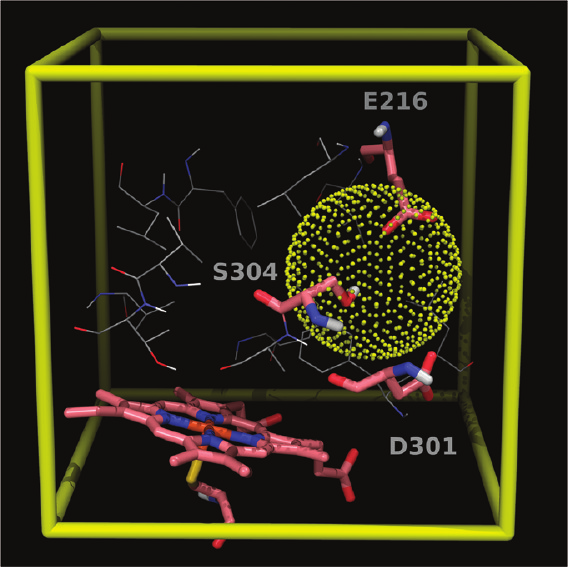
\includegraphics[width=0.35\textwidth]{figures/idsite/glide.png}
\caption{An overview of the entire IDSite procedure.}
\label{fig:idsite_glide}
\end{figure}

% IDSite uses reduced VDW radii for nonpolar atoms both in the protein receptor and the ligand, so that slight steric clashes are tolerated during the docking stage.
% For the protein receptor the VDW scaling factor is fixed at 0.40, while for the ligand, the scaling factor starting from 0.80 is adaptively adjusted until at least 4 valid poses are found.
% With highly flexible ligands and relatively high scaling factors, Glide often finds only a handful of valid poses, and even fewer survive after IDSite screening.
% However, if the scaling factor is set too low, the docked poses may contain too many serious steric clashes, which can cause problems in the subsequent minimization.
% If IDSite fails to find enough valid poses, the scaling factor is adjusted and the number of poses to pass the initial docking phase in Glide is increased accordingly to augment sampling.

% joe is this far
% If the ligand contains other hydrogen-bond donors except for the basic nitrogen, the constrained docking is likely to generate poses that form hydrogen bonds instead of the salt bridge to Glu216 or Asp301.
% However, IDSite is able to distinguish these poses and filter them via an additional salt bridge filter in the pose screening, so that only the poses with a stable salt bridge are allowed to pass to the refinement stage.


\subsection{Monte Carlo Minimization Refinement}
\label{subsection:p450/mcm}
Since the emphasis in IDSite sampling is efficient sampling of low energy conformations, as only the lowest energy conformations are passed on to the next stage of prediction, Monte Carlo Minimization was used instead of a more traditional Monte Carlo simulation because it provides more efficient sampling of low energy conformations (see \ref{subsection:monte_carlo}).
The Monte Carlo Minimization sampling used by IDSite for refinement incorporates three different types of steps: side chain motions, rigid body transformations, and hybrid Monte Carlo simulations.
For each Monte Carlo step, one of three types of motions is selected according to the weighted probabilities, which are different for the two different PLOP sampling stages (see table \ref{table:mmc_params}).
\begin{table}[h]
    \centering
    \begin{tabular}{|c|c|c|}
        \cline{2-3}
        \multicolumn{1}{r|}{~}                       & \multicolumn{2}{c|}{PLOP Sampling Stage} \\
        \cline{2-3}
        \multicolumn{1}{r|}{~}                       & First                        & Second                        \\
        \hline
        Number of Residues Sampled                   & 12                           & 40                            \\
        \vspace{-1.5ex}
        Number of Structures                         & \multirow{2}{*}{max(n*8,24)} & \multirow{2}{*}{max(n*20,60)} \\
        Advanced to Next Stage                       &                              &                               \\
        P(side chain step)                           & 0.5                          & 0.7                           \\
        P(rigid body step)                           & 0.1                          & 0.2                           \\
        P(HMC)                                       & 0.4                          & 0.2                           \\
        \hline
    \end{tabular}
    \caption{The number of residues sampled as well as the number of structures advanced to the next stage from each of the sampling stages.
Also, the relative probabilities of selecting each of the different sampling steps during a Monte Carlo minimization sampling stage.}
    \label{table:mmc_params}
\end{table}

Using the chosen method, a new conformation is proposed and minimized before the Metropolis acceptance criteria (equation \ref{equation:metropolis_acceptance}) is applied to the proposed state, using a temperature of 300 K.
All atoms of all residues with any atom within 5 angstroms of the ligand in the starting crystal structure were allowed to move during Monte Carlo moves, including the ligand itself.

During the minimization Monte Carlo sampling stages of the IDSite procedure, artificial constraints are used to guide the sampling towards a transition state like conformation.
These constraints create artificial bond or angle potentials, which affect the minimization but are not used in the Monte Carlo acceptance test.
For each of the minimization Monte Carlo sampling stages of the IDSite procedure, two different sets of constraints are applied depending on the hybridization of the carbon atom at the possible site of metabolism, for a total of four possible different sets of constraints.
In the first minimization Monte Carlo stage, two constraints are applied, shown in figures \ref{figure:first_sp2_constraints} and \ref{figure:first_sp3_constraints}:
\begin{enumerate}
\item The sulfur-iron-carbon angle is constrained to 145 degrees, with 20 degrees of ``slack'', or a flat bottom to the potential well (denoted as 145\plusorminus20 degrees).
The spring constant of this constraint is about 25 kcal/mol/degree\superscript{2}, or {\textapprox}40\% the strength of a carbon-carbon-carbon angle.
\item A ``dummy'' oxygen atom is placed above the plane of the heme group, in the same position that it would occupy if an oxygen molecule was bound to the heme.  
This dummy atom has no interactions with other atoms, but is used as the anchor of a distance constraint for the carbon at the site of metabolism.  
The carbon-dummy oxygen distance is constrained to 2.5\plusorminus0.5 angstroms.
The spring constant of this constraint is 100 kcal/mol/angstrom\superscript{2}, approximately 1/3rd the strength of a carbon-carbon bond.
\end{enumerate}
\begin{figure}
\centering
\begin{subfigure}[b]{0.35\textwidth}
\centering
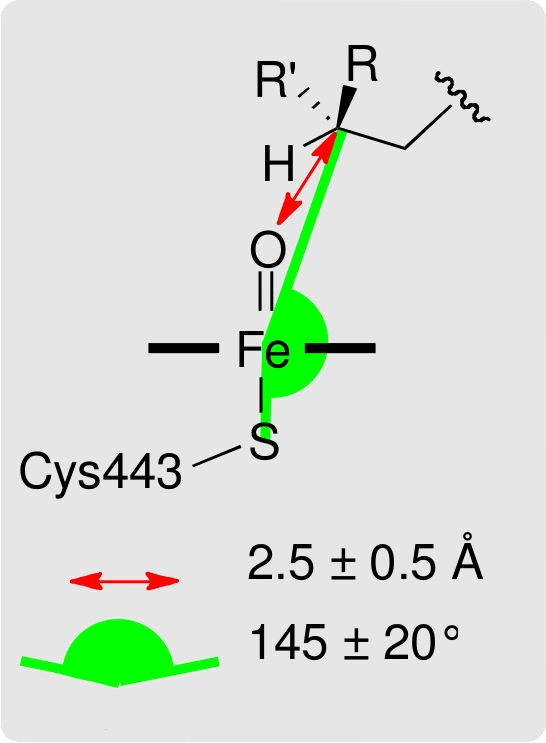
\includegraphics[width=\textwidth]{figures/idsite/33a}
\caption{}
\label{figure:first_sp3_constraints}
\end{subfigure}
\hspace{0.1\textwidth}
\begin{subfigure}[b]{0.35\textwidth}
\centering
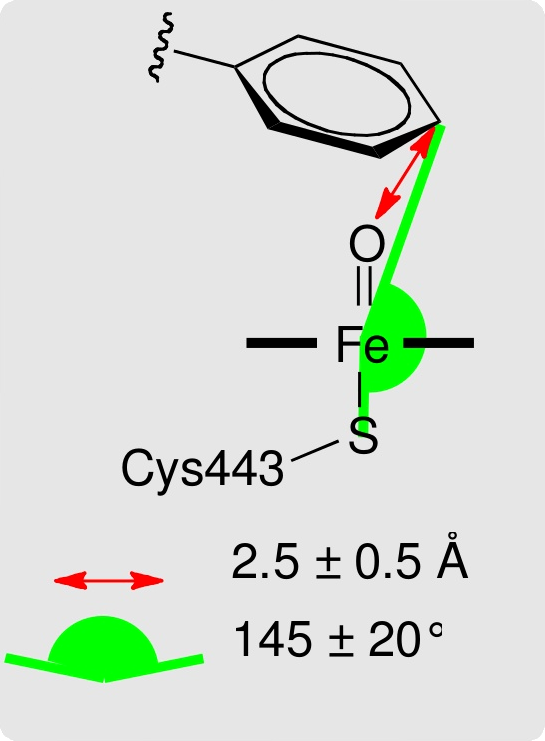
\includegraphics[width=\textwidth]{figures/idsite/33b}
\caption{}
\label{figure:first_sp2_constraints}
\end{subfigure}
\caption{The constraints applied to (a) sp\superscript{3} and (b) sp\superscript{2} atoms during the constrained minimization and first minimization Monte Carlo sampling stage.
The spring constant of the bond constraint (red arrow) is 100 kcal/mol/angstrom\superscript{2}, and that of the angle constraint is 25 kcal/mol/degree\superscript{2}.
The oxygen atom depicted in this figure is a ``dummy'' atom and does not interact with any other atoms in the structure except through the constraint.}
\label{figure:first_constraints}
\end{figure}


In the second minimization Monte Carlo sampling stage, the constraints are different for sp\superscript{2} and sp\superscript{3} carbons.
These constraints are illustrated in figures \ref{figure:second_sp3_constraints} and \ref{figure:second_sp2_constraints}.
For sp\superscript{3} sites:
\begin{enumerate}
\item the hydrogen bound to the carbon at the possible site of metabolism is constrained to a distance of 1.25\plusorminus0.1 angstroms and a spring constant of 20 kcal/mol/angstrom\superscript{2},
\item the carbon in question is constrained to 2.2\plusorminus0.8 angstroms and a spring constant of 10 kcal/mol/angstrom\superscript{2},
\item the heme iron-hydrogen-carbon angle is constrained to 138\plusorminus5 degrees and a spring constant of 20 kcal/mol/degree\superscript{2}.
\end{enumerate}
For sp\superscript{2} sites:
\begin{enumerate}
\item the carbon at the possible site of metabolism is constrained to 1.8\plusorminus0.1 angstroms and a spring constant of 20 kcal/mol/angstrom\superscript{2},
\item both adjacent carbons are also constrained to the dummy oxygen atom, at a distance of 2.5\plusorminus0.1 angstroms and a spring constant of 20 kcal/mol/angstrom\superscript{2}, and
\item finally, the hydrogen bonded to the carbon at the possible site of metabolism is constrained to the oxygen atom at a distance of 2.0\plusorminus0.1 angstroms and a 20 kcal/mol/angstrom\superscript{2} spring constant.
\end{enumerate}
\begin{figure}
    \centering
    \begin{subfigure}[b]{0.35\textwidth}
    \centering
    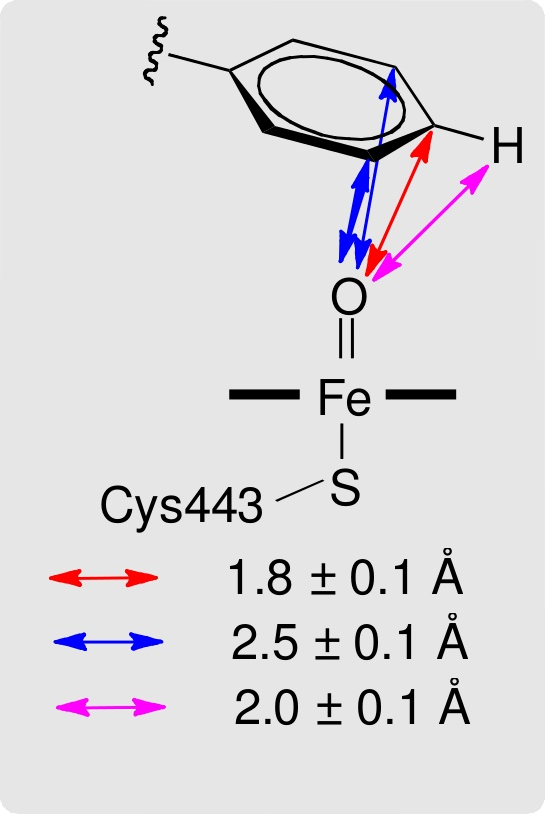
\includegraphics[width=1.0\textwidth]{figures/idsite/34b}
    \caption{}
    \label{figure:second_sp2_constraints}
    \end{subfigure}
    \hspace{0.1\textwidth}
    \begin{subfigure}[b]{0.35\textwidth}
    \centering
    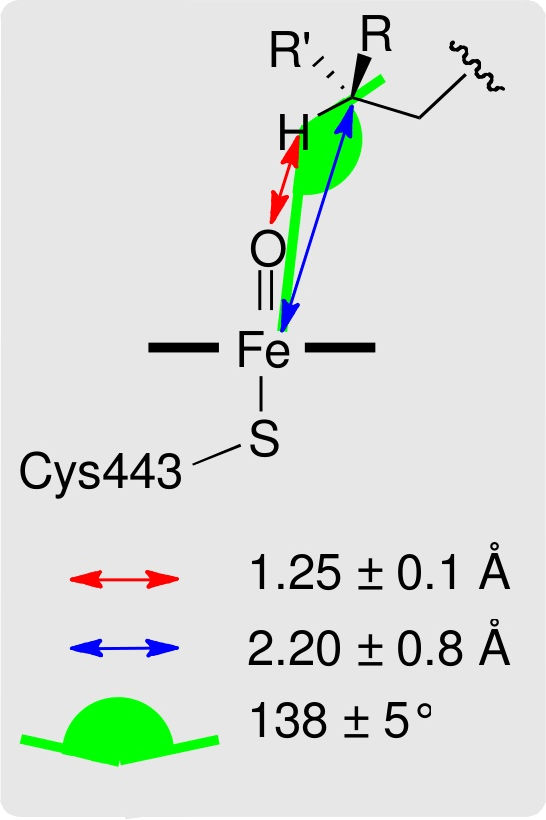
\includegraphics[width=1.0\textwidth]{figures/idsite/34a}
    \caption{}
    \label{figure:second_sp3_constraints}
    \end{subfigure}
    \caption{The constraints applied to (a) sp\superscript{2} and (b) sp\superscript{3} atoms during the constrained minimization and second minimization Monte Carlo sampling stage.}
    \label{figure:second_constraints}
\end{figure}
 

As CYP2D6 forms a conserved salt bridge with the substrate with either glutamate 216 or aspartate 301 \cite{paine2003residues}, this was also incorporated as a constraint during the sampling stages.
In the first sampling stage, this salt bridge is enforced by introducing a harmonic constraint of 3.0\plusorminus0.3 angstroms between the basic nitrogen of the substrate and each of the side chain oxygen atoms in GLU216, ASP301, and SER304 (see figure \ref{figure:salt_bridge_first}).
The spring constants of these constraints are 15.0, 8.0, and 4.0 kcal/mol/angstrom\superscript{2} for GLU216, ASP301, and SER304, respectively.
Additionally, an angle constraint of 150.0\plusorminus30.0 degrees with spring constant of 5.0 kcal/mol/degree\superscript{2} is applied to each of the N-H-O angles.
\begin{figure}[hp]
\centering
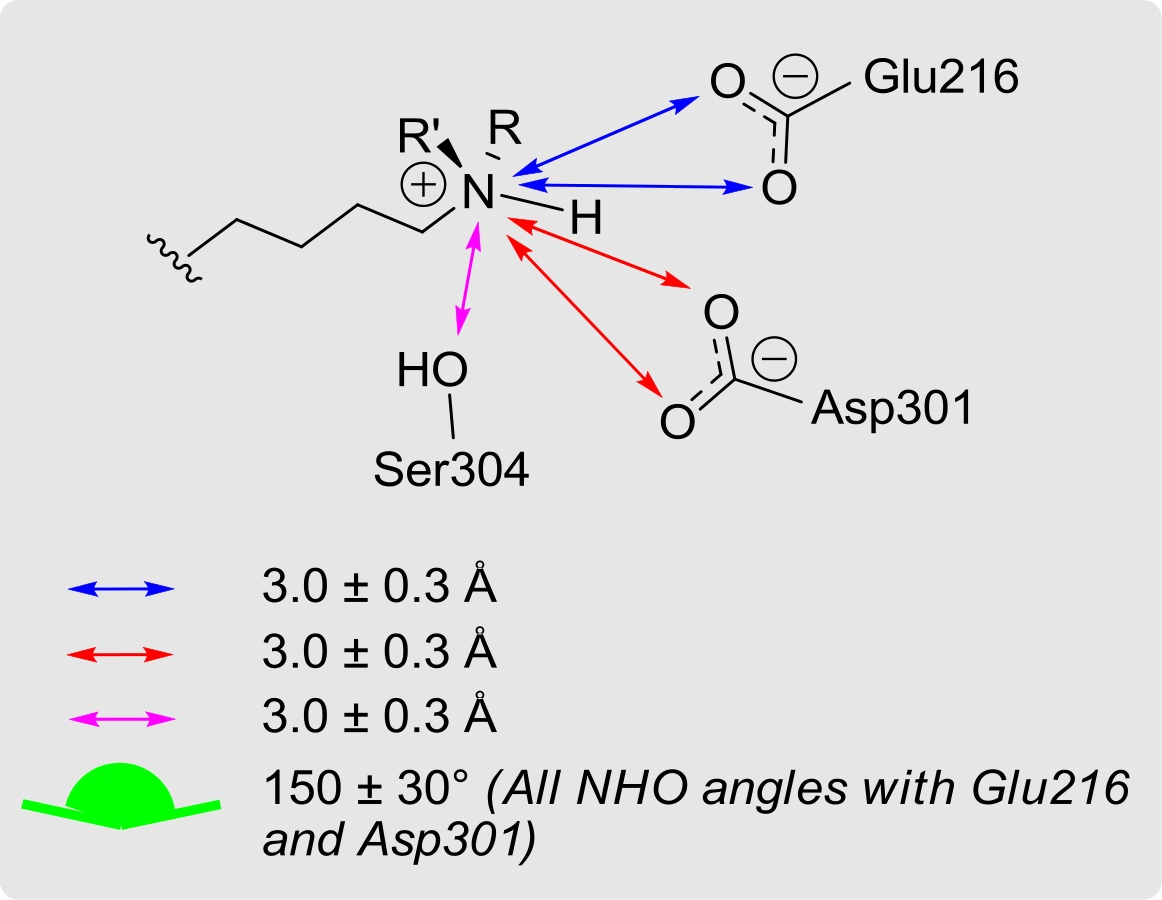
\includegraphics[width=0.50\textwidth]{figures/idsite/salt_bridge_first}
\caption{The constraints applied to the salt bridge region of CYP2D6 during the {\it first} minimization Monte Carlo sampling stage.}
\label{figure:salt_bridge_first}
\end{figure}

In the second sampling stage, four separate trajectories are calculated for each of the four carboxalate oxygens of GLU216, ASP301 (shown in figure \ref{figure:salt_bridge_second}).
In each trajectory a constraint of 1.9\plusorminus0.1 angstroms is applied between the hydrogen attached to the basic substrate nitrogen and one of the four carboxalate oxygens.
Additionally, the angle of the hydrogen bond is constrained to 168\plusorminus12 degrees, with a spring constant of 5.0 kcal/mol/degree\superscript{2}.
\begin{figure}[hp]
\centering
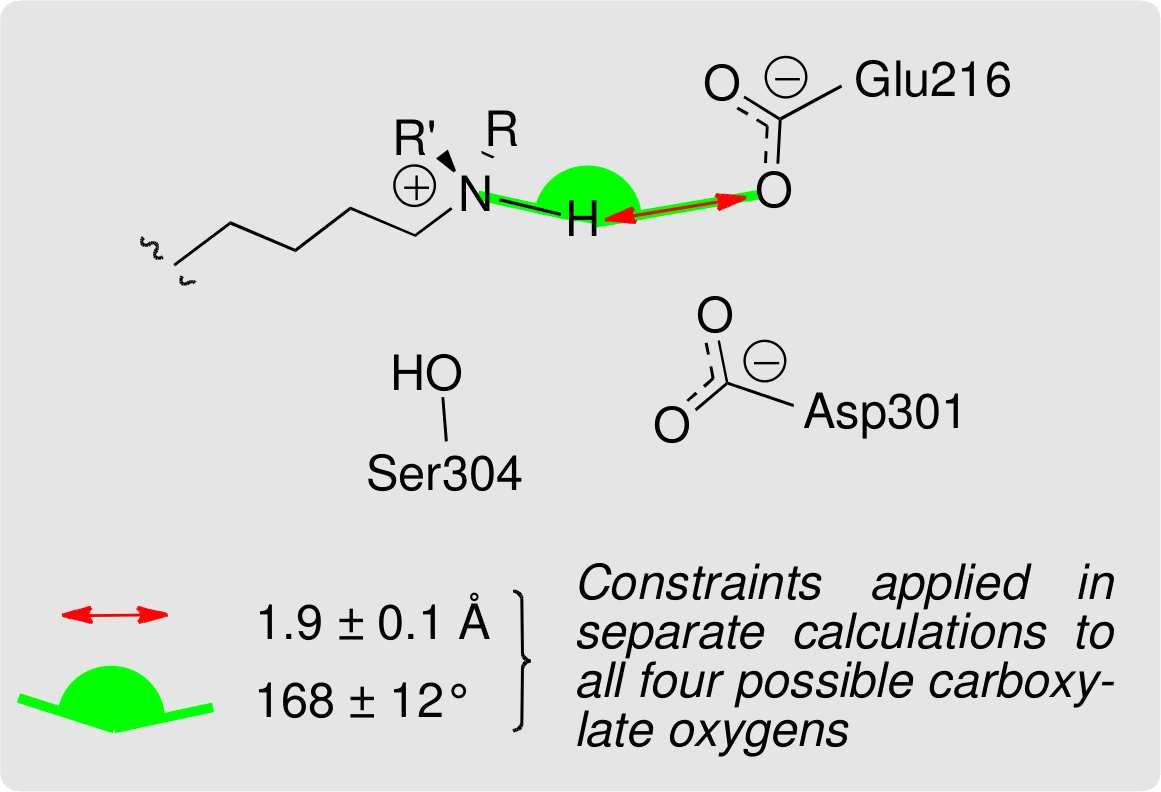
\includegraphics[width=0.50\textwidth]{figures/idsite/salt_bridge_second}
\caption{The constraints applied to the salt bridge region of CYP2D6 during the {\it second} minimization Monte Carlo sampling stage.}
\label{figure:salt_bridge_second}
\end{figure}
 % figure

\begin{figure}[hp]
\centering
\includegraphics[width=0.7\textwidth]{dot_files/mcm_flowchart.png}
\caption{An outline of the Monte Carlo minimization refinement stages in PLOP.}
\label{figure:mcm_flowchart}
\end{figure}

Three different methods of sampling, or moves, were implemented in order to sample different protein-ligand conformations.
A flow chart presenting the minimization Monte Carlo procedure is presented in figure \ref{figure:mcm_flowchart}.
\begin{enumerate}
\item Side chain moves.
Several types of side chain motions were implemented in PLOP.
In all cases, they are defined in a such a way that they can be applied to both ligands and proteins.
The same atomic overlap screening function implemented with the rigid body Monte Carlo was implemented with the side chain torsional moves.
a. Random torsion angle moves: The first type of move that was implemented is random movement of torsional chi angles.
For small torsion moves, a random perturbation of the angle of +/- X is made, where X is a random number with user defined magnitude.
For large torsion moves, for each torsion angle that is changed, a random angle is selected in the form 60*Y +/- X, where Y = 1 through 5, and X is the same random number for the small torsion moves.
The large move was introduced since positions at the top of rotamer barriers are relatively unlikely to be selected, and efficiency thus can be improved by focusing on the more probable moves.
The ratio of small to large torsion moves can be used-adjusted, as can the ratio of probabilities of changing all the torsions in a randomly selected side chain versus changing only one single (randomly selected) torsion among all the free torsions in the simulation can be set as a user-defined parameter.
Rotamer side chain moves: A second type of torsional samples implemented is random selection of a new rotamer state for the entire side chain, plus an optional user defined small noise term for each torsion in the rotamer state.
A database of protein rotamer states obtained from crystallographic data are already a part of PLOP \cite{xiang2001extending} Rotamer libraries for ligands are generated by examining all possible side chain conformations at 10 degree resolution and screening this set for steric clashes.
A Monte Carlo move in this case represents a choice of a new torsional rotamer state for the entire side chain.
Monte Carlo moves based on torsional states cannot lead to correct equilibrium distributions, as transitions from non-rotamer states to rotamer states are defined, but not reverse transitions, upsetting detailed balance.
However, a pretabulated rotamer state is more likely to be low energy than a randomly generated torsional state, and thus allows for more diverse conformational searching.
Correlated torsional moves: Most torsional rearrangements of the side chains in the core of proteins are highly correlated because of the density.
In order to attempt to include correlated torsional motion, at each step we examine the distance between all pairs of beta carbons in the ligands that are free to move.
At each step, for the set of side chains that are free to move, clusters where beta carbons are all mutually within a user-specified distance are identified.
This process takes a trivial amount of time compared to an energy evaluation, so does not slow the simulation at all.
Then, with user specified probabilities, clusters of different sizes are selected for the torsional moves, either with random side chain moves, or rotamer selection moves.
By selecting only clusters where all residues are mutual neighbors, detailed balanced is observed for simulations where accurate equilibrium sampling is desired.
By varying the dihedral angles of the rotatable bonds, IDSite uses side chain MC moves in PLOP to sample the selected side-chain conformations of the protein and of the ligand.
Up to three close residues (C beta distance within 6 angstroms) are allowed to rotate collectively, but the moves of the protein residues and those of the ligand are separated.
In each attempted movement, the conformations of the selected side chains (from the protein/ligand) are either changed by random perturbations or assigned by the randomly selected rotamers from a library.
For an attempt with a random perturbation, the displacement of each dihedral angle is the sum of a large rotation (N times 60 degrees with N as a random integer between 0 and 5) and a random perturbation from 0 to 30 degrees.
For a rotamer library attempt, a side-chain conformation is updated with a random rotamer from a high resolution side-chain library for protein residues \cite{xiang2001extending}, and from a homogeneous library at 10 degree resolution for the ligand.
If a structure with tolerable overlaps is generated in an attempt, it is minimized and sent to subsequent stages for judgment of acceptance.
Each side-chain move takes less than 15 seconds and is the fastest among all the three move types.

% from mike's
For side chain Monte Carlo, a steric screen with an overlap factor of 0.6 was used.
Rotamer torsional moves were selected 75\% of the time, with half of the remaining being of random torsions, and the other half random perturbations of all torsions within the randomly selected side chains.
Clusters of size 1 (i.e. single side chains), size 2 and size three were selected in equal proportion, and all side chains in the cluster were perturbed with the selected torsion move.
A mutual beta carbon distance of 6 Angstroms was used for the clustering size.
Small torsion perturbations made +/- 60 degress from the current dihedral angle, and were performed 5\% of the time; Large periodic moves were performed 95\% of the time.
Only outer steps were performed, and each side chain Monte Carlo series consisted in only one move.
Minimization was performed after the single step, and acceptance was performed at 1 K.


\item % TODO
Rigid motion moves.
Rigid body translation and rotation were also implemented for noncovalently linked moieties, such as ligands.
Random rotations and translations were coupled together, allowing for more concerted movement.
Rigid body move implemented in PLOP can optionally include a screening step, where atomic Lennard-Jones overlaps that would lead to energies much higher than would be observed in any conceivably long equilibrium simulation are rejected without further evaluation.
A ratio of 0.7 between the distance between the two atoms and the sum of the Lennard-Jones radii of the two atoms yields energies on the order of 10's of thousands of kcal/mol, and is thus reasonable to maintain equilibrium sampling in a Monte Carlo simulation.
Translations were implemented in a random direction, with a user-defined magnitude.
Rotations were implemented by picking a random quarternion (a random angle around a random axis, through the geometric center of the rigid group) with a user specified maximum random angle centered around either the current angle, or 180 from the current angle, in the case of a flip.
Multiple time scale Monte Carlo sampling was also implemented with rigid body moves, with short range and long range interactions defined as above.
In addition, an option to compute the inner Monte Carlo loops with reduced Lennard-Jones radii were also implemented, to increase the ability to escape from tight spacial bottlenecks.
In this case, the long time step energies are the full energies with unscaled Lennard-Jones radii.
This increases the conformational freedom and therefore sampling for the short, at a cost of decreasing the acceptance probability in the outer loop.
Scaled Lennard-Jones radii were also implemented in multiple time dynamics, but yielded very little apparent improvement because of the lack of phase space overlap between dynamics with different scaled Lennard-Jones radii).
Rigid body moves are used to sample the translational and rotational space of the ligand.
Multiple attempts with reduced VDW radii are applied, as it is quite common to fail in searching for a clash-free conformation in a single rigid body moving attempt (especially when the ligand is large and flexible and the binding pocket is relatively small).
Each rigid body move includes 1000 attempts, and each attempt performs a translation along a random vector and a rotation around a random axis, with less than 0.5 angstroms and 60 degree displacement, respectively.
In addition, the VDW radii are reduced (scaling factor 0.8) to soften the Lennard-Jones potential, so that mild steric clashes are allowed, which are likely to be resolved by the subsequent minimization.
The rigid body move usually takes 20 to 40 seconds per move.

% from mike's
For rigid body Monte Carlo, a steric screen with an overlap factor of 0.7 was used, with a translation size of 0.5 Angstroms and a rotation size of plus or minus 60 degrees.
No flip moves were included, as flips were not anticipated with the geometry of the ligand system [Robert, check this is true?] A Lennard-Jones scaling parameter of 0.8 was used during the inner steps.
Each rigid MC step consisted of 1000 inner steps, and only one outer step, meaning that only one minimization occurred each time rigid body Monte Carlo was selected as the move step.


\item The Hybrid Monte Carlo (HMC) \cite{duane1987hybrid} step is a velocity verlet molecular dynamics simulation.
This simulation allows all atoms in both the ligand and residues containing atoms withing 5 angstroms of the ligand to move.
Initial velocities are taken from a Maxwell-Boltzmann distribution at 900 K.
Bonded and short range interactions evaluated every 1 nanosecond inner time step, and long range potentials are assumed to be fixed over inner steps.
Five inner steps compose each outer HMC step.
In the outer step the molecular surface, long range interactions and, Born alphas are updated before computing the energy and applying the Metropolis acceptance criteria at a temperature of 900 K after each MD run.
Taking up to 15 minutes per move, the HMC is the most expensive among all three types of moves in PLOP.

%, with long range interactions evaluated every long time step.
%In this case, molecular dynamics is run only using only the short range energies, which will conserve energy and thus yield proper Markov chain behavior while the cutoffs and Born alpha are not updated.
%Inner loop Monte Carlo steps are performed with only the short range dynamics, and outer loop Monte Carlo steps are performed with all interactions.
%In the case of implicit solvent simulations, the Born alpha are only reevaluated in the outer loop Monte Carlo steps.
%This allows for evaluation of the full surface integral relatively infrequently, and yields a properly weighted Boltzmann distribution of conformations without needing position derivatives of the Born alphas.

%Energies are conserved in vacuum simulations if the long range cutoff extends to cover the entire molecule.
%With implicit solvent dynamics, energies are not conserved as there is no derivative of the Born alpha with respect to position, so a thermostat must be used to approximate realistic dynamics.
%One mode of action is to run HMC on top of normal RESPA dynamics, with acceptance and rejections done after a fixed number of steps of MD, as in typical HMC.
%Velocities are re-randomized after every Monte Carlo step from the Maxwell-Boltzmann distribution.
%However, HMC can also be implemented in a multiple-time step Monte Carlo framework \cite{hetenyi2002multiple}.
%The hybrid Monte Carlo (HMC)\cite{duane1987hybrid} move in PLOP performs simultaneous sampling for the selected residues in the protein side chains and backbone as well as the ligand.
%Each HMC move performs a 5 picosecond, constant energy molecular dynamic (MD) simulation (starting at 900K) on all the atoms in the selected residues.
%Taking up to 15 minutes per move, the HMC is the most expensive among all three types of moves in PLOP.

%The underlying molecular dynamics for the hybrid Monte Carlo consisted of 500 5 ns RESPA \cite{tuckerman1991molecular} steps, each with 5 1 ns short range steps.
%The dynamics were initialized from a Maxwell-Boltzmann distribution at 900 K, and then run without any thermostat the full 2.5 ps run.
%Minimization was performed after the single HMC step, with acceptance/rejection performed at a Monte Carlo temperature of 900 K.

% is built on top of a molecular dynamics (MD) integrator.
% We implemented velocity verlet MD using the RESPA formalism \cite{tuckerman1991molecular}, with bonded and short range interactions evaluated every inner time step, with long range interactions evaluated every long time step.
% We also included in the including Andersen, Berendsen, and Langevin thermostats, as well as Brownian Dynamics.
% Short range interactions included all bonded interactions and nonbonded interactions less than a user-specified cutoff.
% Both short and long range cutoffs are dipole-based as described in a previous paper [cite].
% and then run without any thermostat the full 2.5 ps run.

\end{enumerate}

\subsection{Evaluation}
\label{subsection:p450/evaluation}
Both a parameterized and an unparameterized model were used to classify potential sites of metabolism.
IDSite makes the assumptions that all intermediates before the rate determining step are at equilibrium \cite{wang2007stochastic}, that hydrogen abstraction is the rate limiting step for hydroxilation of aliphatic carbons and electrophilic attack is the rate limiting step for hydroxilation of aromatic rings \cite{guengerich2001common,shaik2005theoretical}.
With these assumptions the rate of metabolism at each possible site of reaction is affected by the free energy of binding in order to put that site in the site of reaction, as well as the free energy barrier of rate determining step, or
\input{equations/curtin_hammett} % dG = dG bind + dG react
The ${\Delta}G_{\mathrm{binding}}$ above is calculated using a PLOP evaluation of the refined pose.
The intrinsic reactivity for the system is computed from DFT calculations on a simplified system, replacing the heme with a methody radical, and using a linear relationship between $IR(\mathrm{heme})$ and $IR(\mathrm{methoxy\ radical})$ to estimate the true reactivity for the heme system.
\begin{figure}[h]
\centering
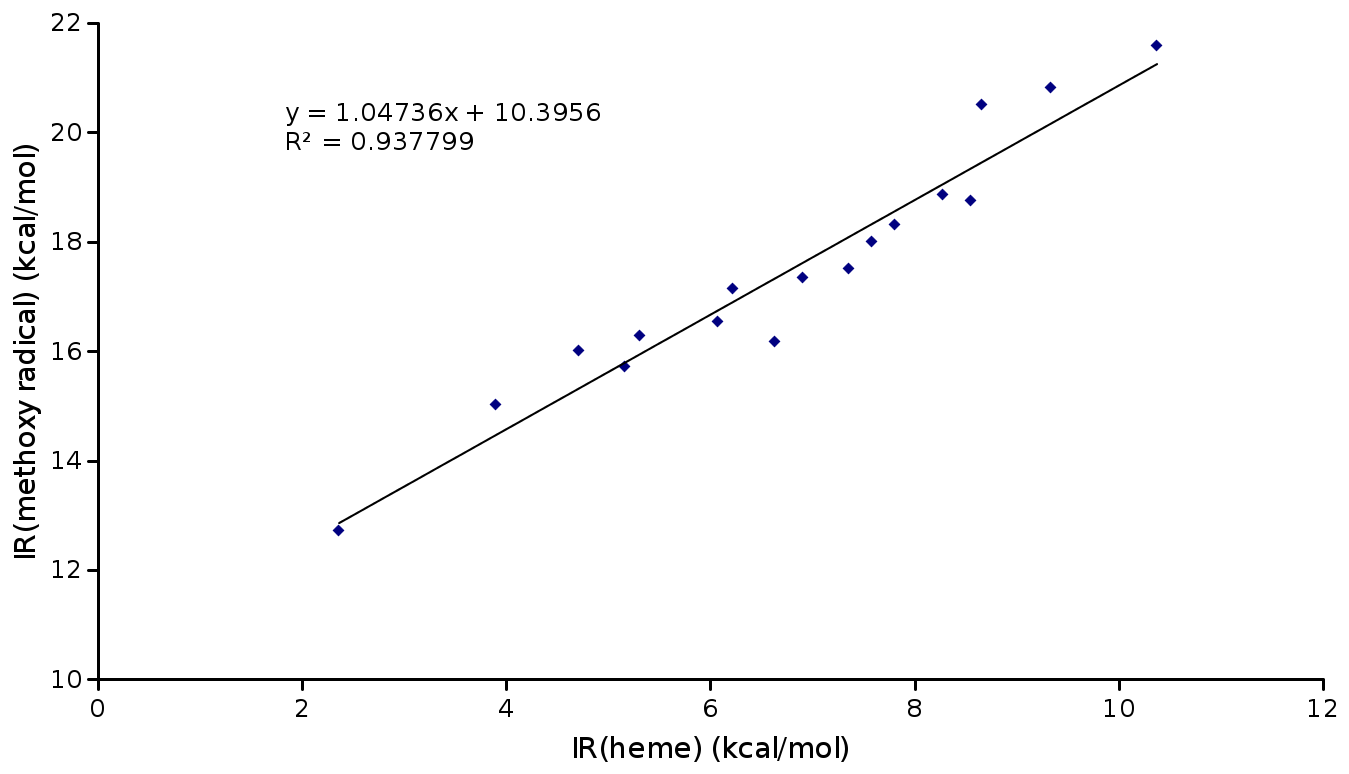
\includegraphics[width=0.8\textwidth]{figures/idsite/intrinsic_corrected.png}
\label{fig:idsite/intrinsic}
\caption{The linear relationship between the calculated intrinsic reactivity of the methoxy radical complex and that of the heme complex.
Adapted from \protect\cite{li2011idsite} with minor correction.
In the original manuscript the slope of the regression was reported as 1.117 and that number was used throughout.
This difference should not significantly affect the physical IDSite classifier results, and does not affect the results of the fit model.
In the rest of this text the value from the original publication of 1.117 will be used.}
\end{figure}
\input{tables/heme_methoxy.tex}
\input{equations/intrinsic_reactivity} % estimate from abbreviated reactivity
Since this constant $C$ is identical for each state it has no effect on the relative differences in ${\Delta}G_{\mathrm{site}}$ or the relative rate of metabolism at possible sites.
\input{equations/g_site} % E/G equation
Since the ligand is forced to assume a different conformation in order to react, the energy of this transition state conformation, $E_{\mathrm{TS}}$, is also computed using PLOP.
As the relative abundance of different metabolites is determined by differences in ${\Delta}G$ per site rather than absolute reactivities, the constant in equation \ref{equation:g_site} does not affect which metabolites are produced.
A site of possible metabolism is classified as positive if it is observed in greater than 0.1\% yield, which corresponds to a \ddg\ of \textapprox4.75 kcal/mol between the most favored state and the cutoff for negative predictions. 

The second classifier is similar however:
\begin{enumerate}
\item a different constant is used to estimate $IR(\mathrm{heme})$ from $IR(\mathrm{methoxy\ radical})$, namely 1.071,
\item if the binding energy of the transition state complex of a pose is within 5.26 kcal/mol of the lowest pose, it is set to the binding energy of the lowest pose.
Otherwise the difference is scaled by 0.58,
\item and the cutoff for an active prediction is changed from 4.75 kcal/mol to 1.46 kcal/mol.
\end{enumerate}
These parameters were decided upon by maximizing $\frac{\mathrm{true\ positives}}{(\mathrm{false\ positives + false\ negatives})}$ on a training set of 36 compounds.


\section{Results}
\label{section:p450/results}
Both physical and fitted IDSite were able to acheive promising results predicting CYP2D6 sites of metabolism.

The physical model correctly identified 68 of 82 active sites of metabolism for a sensitivity of 0.829.
For inactive sites this model correctly identified 1054 of 1075 inactive sites with a specificity of 0.980.
The fit model performed similarly, and even slighly better identifying 52 of 57 sites of metabolism (sensitivity of 0.912) in the training set and 25 of 25 in the test set (sensitivity of 1.0).
\begin{equation}
\mathrm{sensitivity} = \frac{TN}{TN + FP} = \frac{\text{\# of true sites of non-metabolism identified}}{\text{\#\ experimental\ sites\ of\ non-metabolism}}
\end{equation}

\begin{equation}
\mathrm{sensitivity} = \frac{TP}{TP + FN} = \frac{\text{\#\ of\ true\ sites\ of\ metabolism\ identified}}{\text{\#\ experimental\ sites\ of\ metabolism}}
\end{equation}

\begin{table}[h]
\singlespace
\footnotesize
\centering
\begin{tabular}{cccccccccc}
\hline
	&	&Physical	&	&	&Fitted	&	&	&	&\\
Compound \#	&Compound Name	&TP	&FP	&FN	&TP	&FP	&FN	&	&\\
\hline
1	&4-methoxyamphetamine	&1	&0	&0	&1	&0	&0	&	&\\
2	&Amitriptyline	&2	&2	&0	&2	&0	&0	&	&\\
3	&Aprindine	&4	&0	&1	&5	&0	&0	&	&\\
4	&Brofaromine	&1	&0	&0	&1	&0	&0	&	&\\
5	&Bufuralol	&0	&1	&1	&1	&0	&0	&	&\\
6	&Carvedilol	&1	&0	&2	&2	&0	&1	&	&\\
7	&Cinnarizine	&0	&2	&1	&0	&2	&1	&	&\\
8	&Clomipramine	&1	&0	&1	&1	&0	&1	&	&\\
9	&Codeine	&1	&0	&0	&1	&0	&0	&	&\\
10	&Desipramine	&2	&0	&0	&2	&0	&0	&	&\\
11	&Dextromethorphan	&1	&0	&0	&1	&0	&0	&	&\\
12	&Dihydrocodeine	&1	&1	&0	&1	&0	&0	&	&\\
13	&Ethylmorphine	&1	&0	&0	&1	&0	&0	&	&\\
14	&Flunarizine	&1	&0	&0	&1	&0	&0	&	&\\
15	&Fluperlapine	&1	&0	&0	&1	&0	&0	&	&\\
16	&Hydrocodone	&1	&0	&0	&1	&0	&0	&	&\\
17	&Imipramine	&2	&0	&0	&2	&0	&0	&	&\\
18	&Indoramine	&1	&0	&0	&1	&0	&0	&	&\\
19	&MDMA	&1	&0	&0	&1	&0	&0	&	&\\
20	&Methamphetamine	&1	&0	&0	&1	&2	&0	&	&\\
21	&Methoxyphenamine	&2	&0	&0	&2	&0	&0	&	&\\
22	&Metoprolol	&1	&0	&1	&2	&0	&0	&	&\\
23	&Mexiletine	&2	&0	&1	&2	&0	&1	&	&\\
24	&Mianserin	&1	&0	&0	&1	&0	&0	&	&\\
25	&Mirtazapine	&0	&1	&1	&1	&1	&0	&	&\\
26	&Nortriptyline	&1	&1	&0	&1	&0	&0	&	&\\
27	&Ondansetron	&2	&0	&0	&1	&0	&1	&	&\\
28	&Paroxetine	&1	&0	&0	&1	&0	&0	&	&\\
29	&Perhexiline	&2	&0	&0	&2	&0	&0	&	&\\
30	&Propafenone	&1	&1	&0	&1	&1	&0	&	&\\
31	&Propranolol	&2	&2	&0	&2	&1	&0	&	&\\
32	&Tamoxifen	&1	&0	&0	&1	&0	&0	&	&\\
33	&Terfenadine	&3	&0	&0	&3	&0	&0	&	&\\
34	&Tiracizine	&1	&2	&0	&1	&1	&0	&	&\\
35	&Tropisetron	&2	&0	&1	&3	&0	&0	&	&\\
36	&Venlafaxine	&1	&0	&0	&1	&0	&0	&	&\\
	&TOTAL	&47	&13	&10	&52	&8	&5	&	&\\
\hline
\end{tabular}
\caption{Results of physical and fitted IDSITE on training set of 36 compounds.}
\label{table:p450_training}
\end{table}

\begin{table}[h]
\singlespace
\footnotesize
\centering
\begin{tabular}{cccccccc}
\hline
 &  &  & Physical &  &  & Fitted & \\
Compound \# & Compound & TP & FP & FN & TP & FP & FN \\
\hline
37 & Atomoxetine & 0 & 1 & 1 & 1 & 2 & 0 \\
38 & Bicifadine & 1 & 2 & 0 & 1 & 0 & 0 \\
39 & Bupranolol & 1 & 0 & 0 & 1 & 0 & 0 \\
40 & Carteolol & 1 & 1 & 0 & 1 & 0 & 0 \\
41 & Chlorpromazine & 1 & 0 & 0 & 1 & 0 & 0 \\
42 & EMAMC & 1 & 0 & 0 & 1 & 0 & 0 \\
43 & Encainide & 1 & 1 & 0 & 1 & 1 & 0 \\
44 & Harmaline & 1 & 0 & 0 & 1 & 0 & 0 \\
45 & Harmine & 1 & 1 & 0 & 1 & 1 & 0 \\
46 & Ibogaine & 1 & 0 & 0 & 1 & 0 & 0 \\
47 & MAMC & 1 & 0 & 0 & 1 & 0 & 0 \\
48 & MMAMC & 1 & 0 & 0 & 1 & 0 & 0 \\
49 & MOPPP & 1 & 0 & 0 & 1 & 0 & 0 \\
50 & Oxycodone & 1 & 0 & 0 & 1 & 0 & 0 \\
51 & Spirosulfonamide & 2 & 0 & 0 & 2 & 0 & 0 \\
52 & Timolol & 2 & 0 & 2 & 4 & 0 & 0 \\
53 & Tolterodine & 0 & 1 & 1 & 1 & 1 & 0 \\
54 & Tramadol & 1 & 1 & 0 & 1 & 1 & 0 \\
55 & Tyramine & 2 & 0 & 0 & 2 & 0 & 0 \\
56 & Zotepine & 1 & 0 & 0 & 1 & 0 & 0 \\
 & Total & 21 & 8 & 4 & 25 & 6 & 0 \\
\hline
\end{tabular}
\caption{Results of physical and fitted IDSite on a test set of 20 compounds.
Note that for the physical model there is no training performed so results in the text are presented in a unified fashion for the training and test set.}
\label{table:p450_testing}
\end{table}






The fit model also correctly identified 709 of 717 inactive sites in the training set (specificity of 0.989) and 352 of 358 inactive sites in the test set (specificity of 0.983).
As the performance of the fit model is similar to that of the physical model, it does not appear that the fit model is overparameterized to the training set.
Specific results for both models are presented in Tables \ref{table:p450_training} and \ref{table:p450_testing}, and the specific sites identified by both models as well as experiments are illustrated in Figures \ref{fig:idsite_traininga} and \ref{fig:idsite_test}. 

We believe that the parameters help account for some degree of noise in the molecular mechanics calculations.
The scaling of the binding energy difference, either to zero inside a window about the minimum energy pose, or by a factor of 0.58 decreases the relative weight of the molecular mechanics contribution relative the quantum contribution to the classifier.
This might imply that some sites are not being classified as active because they are not in the lowest energy conformation around the docked pose, suggesting that additional molecular mechanics sampling might further improve results.
However as will be discussed later, the molecular mechanics stage already dominates the total time necessary for an IDSite prediction, and the current molecular mechanics procedure takes about 450 hours.   

\begin{figure}
\centering
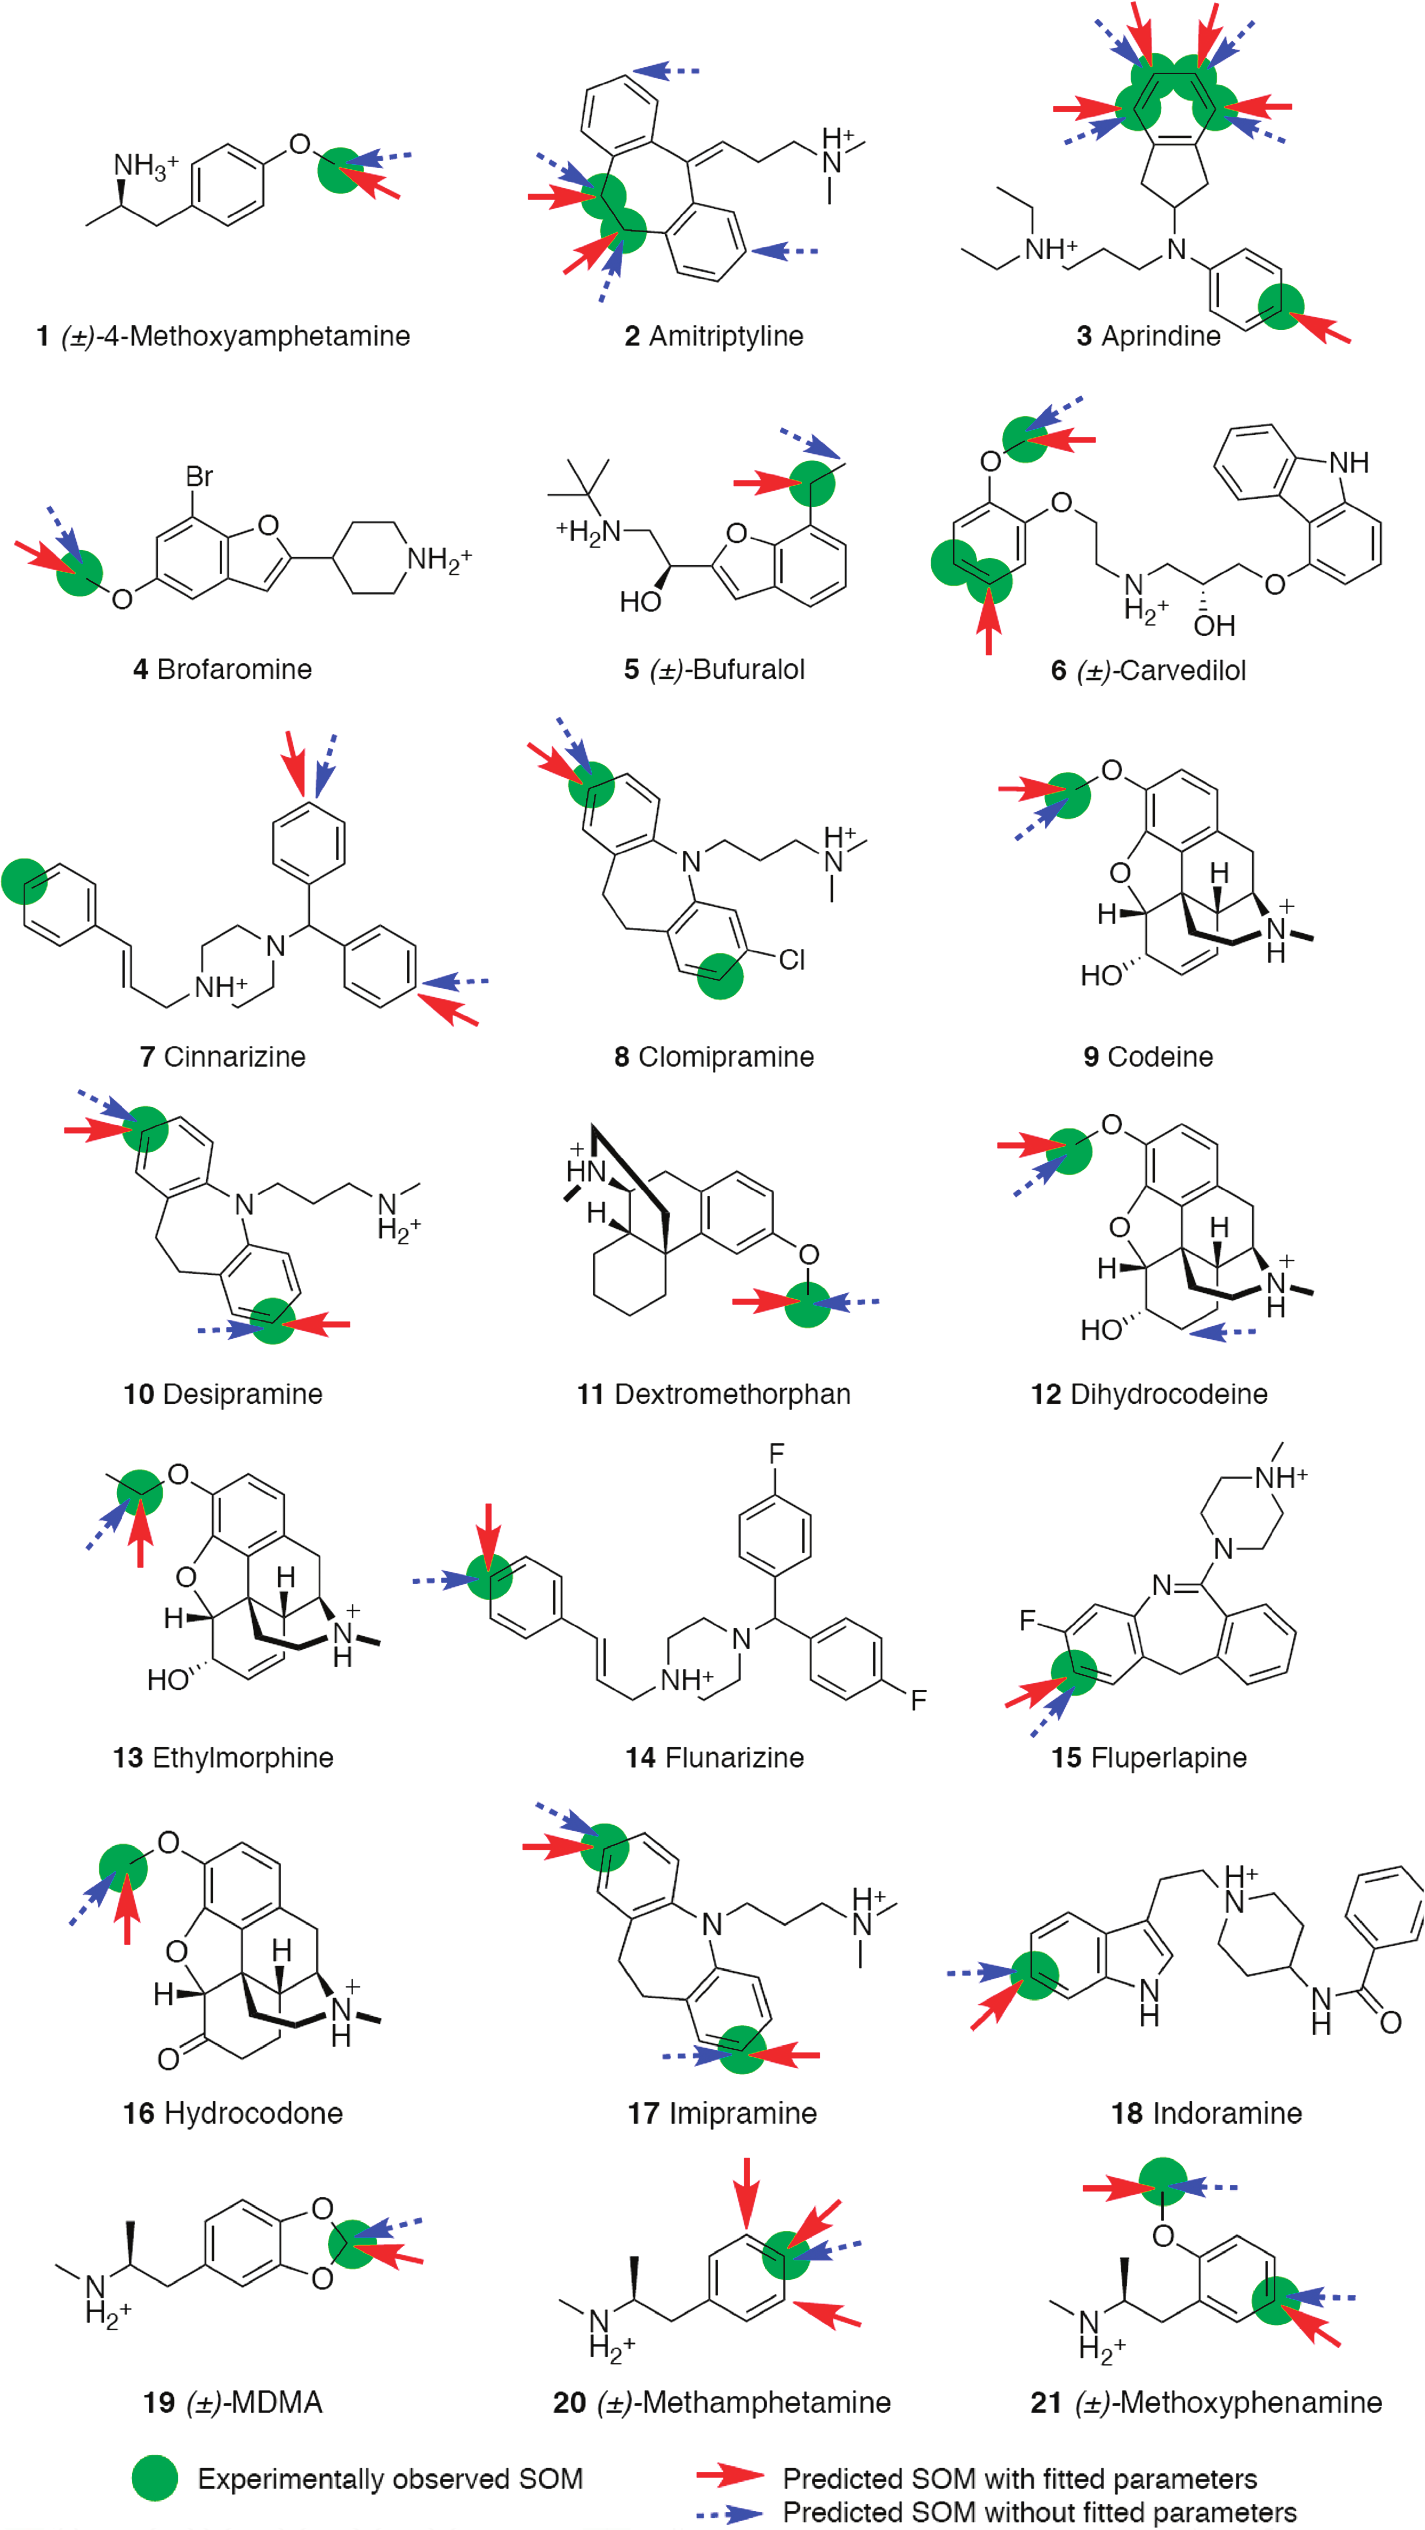
\includegraphics[width=0.65\textwidth]{figures/idsite/idsite_figure-007.png}
\caption{Physical and fitted IDSite predictions of sites of metabolism on the training set.}
\label{fig:idsite_traininga}
\end{figure}

\begin{figure}
\ContinuedFloat
\centering
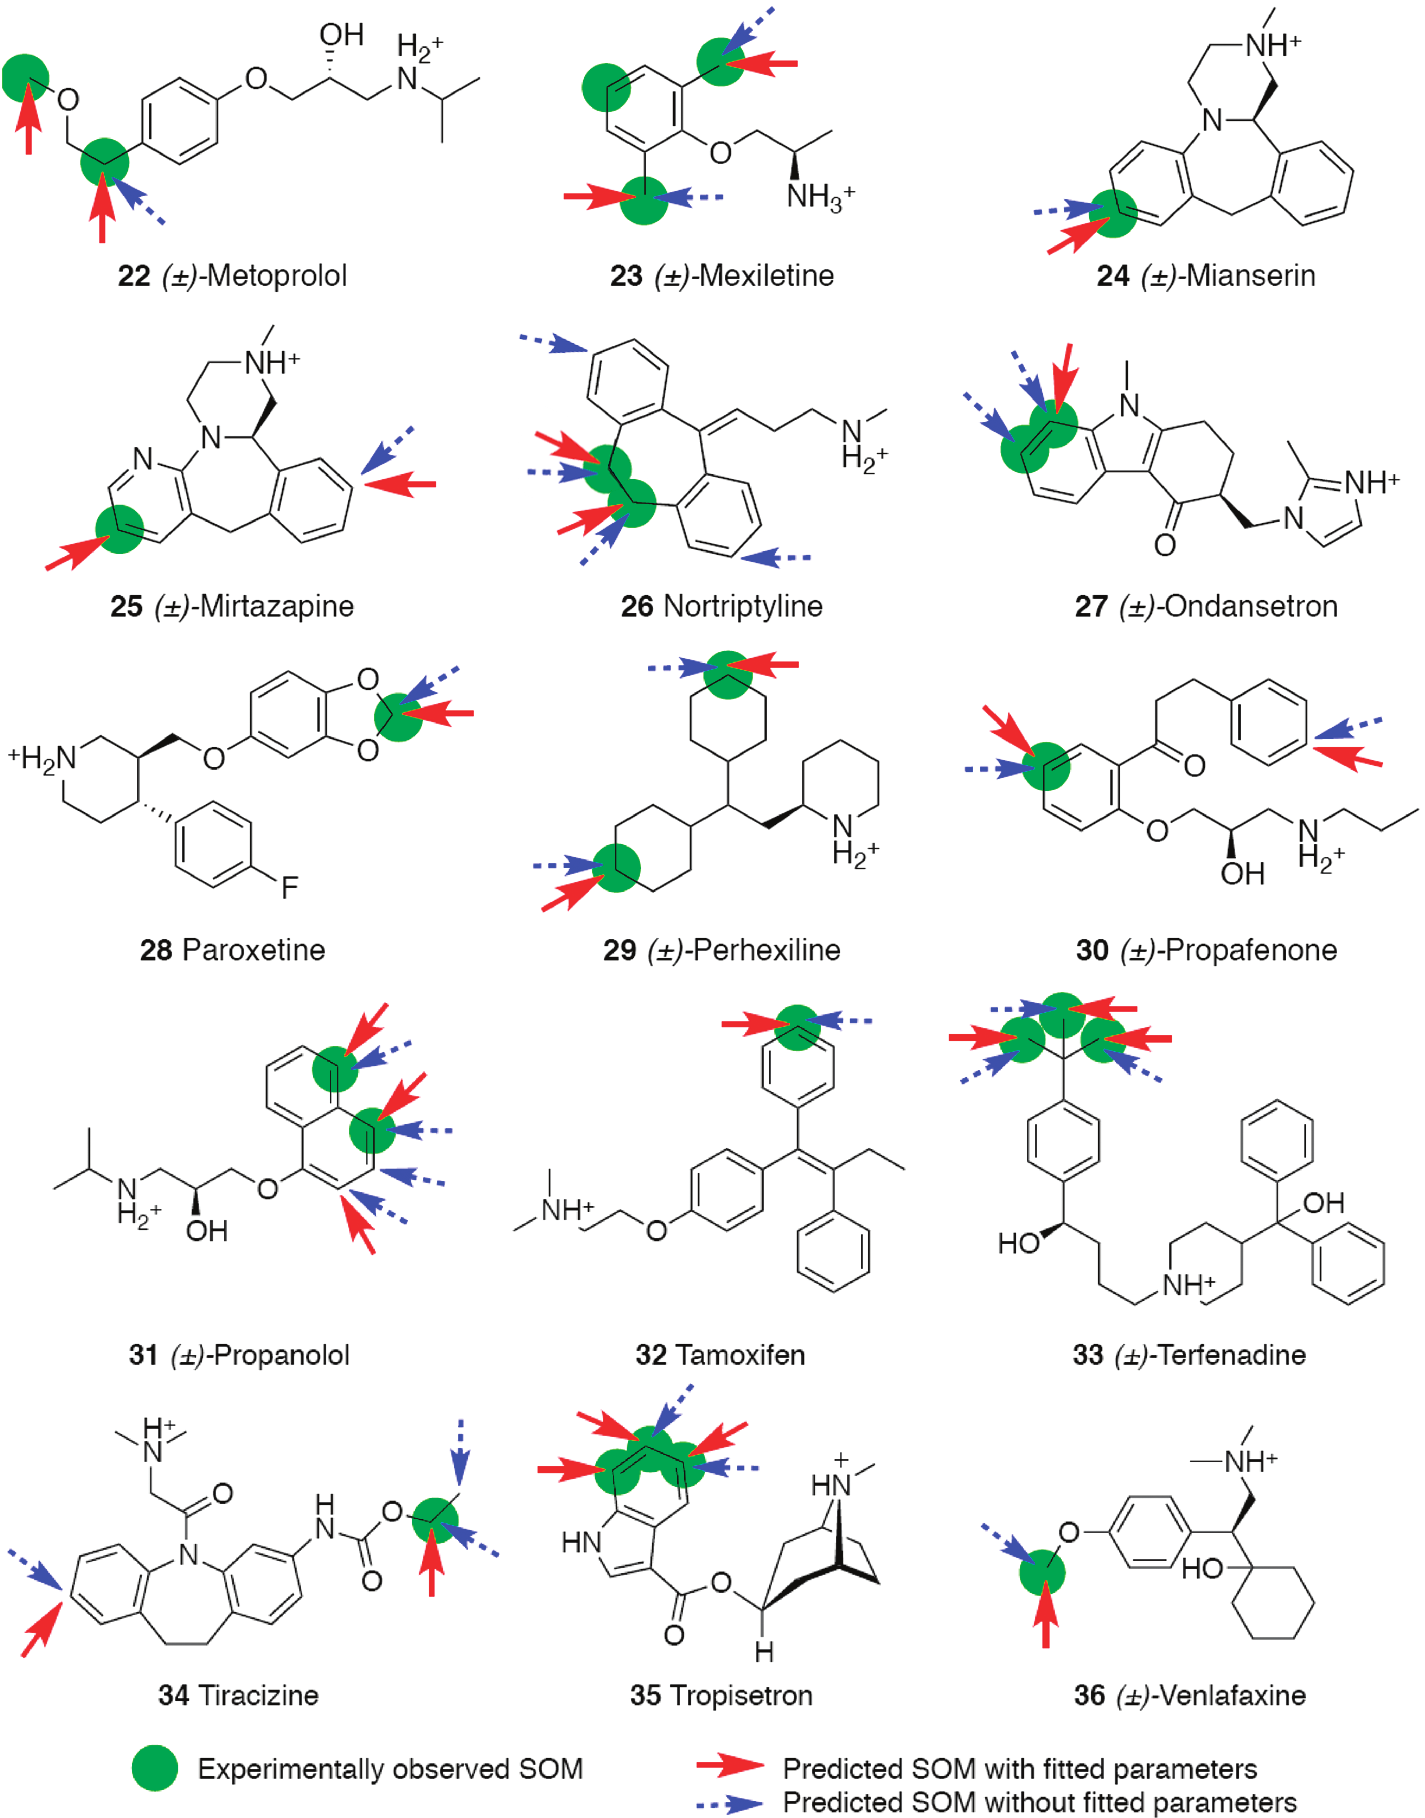
\includegraphics[width=0.65\textwidth]{figures/idsite/idsite_figure-008.png}
\caption{(continued)}
\label{fig:idsite_trainingb}
\end{figure}


\begin{figure}
\centering
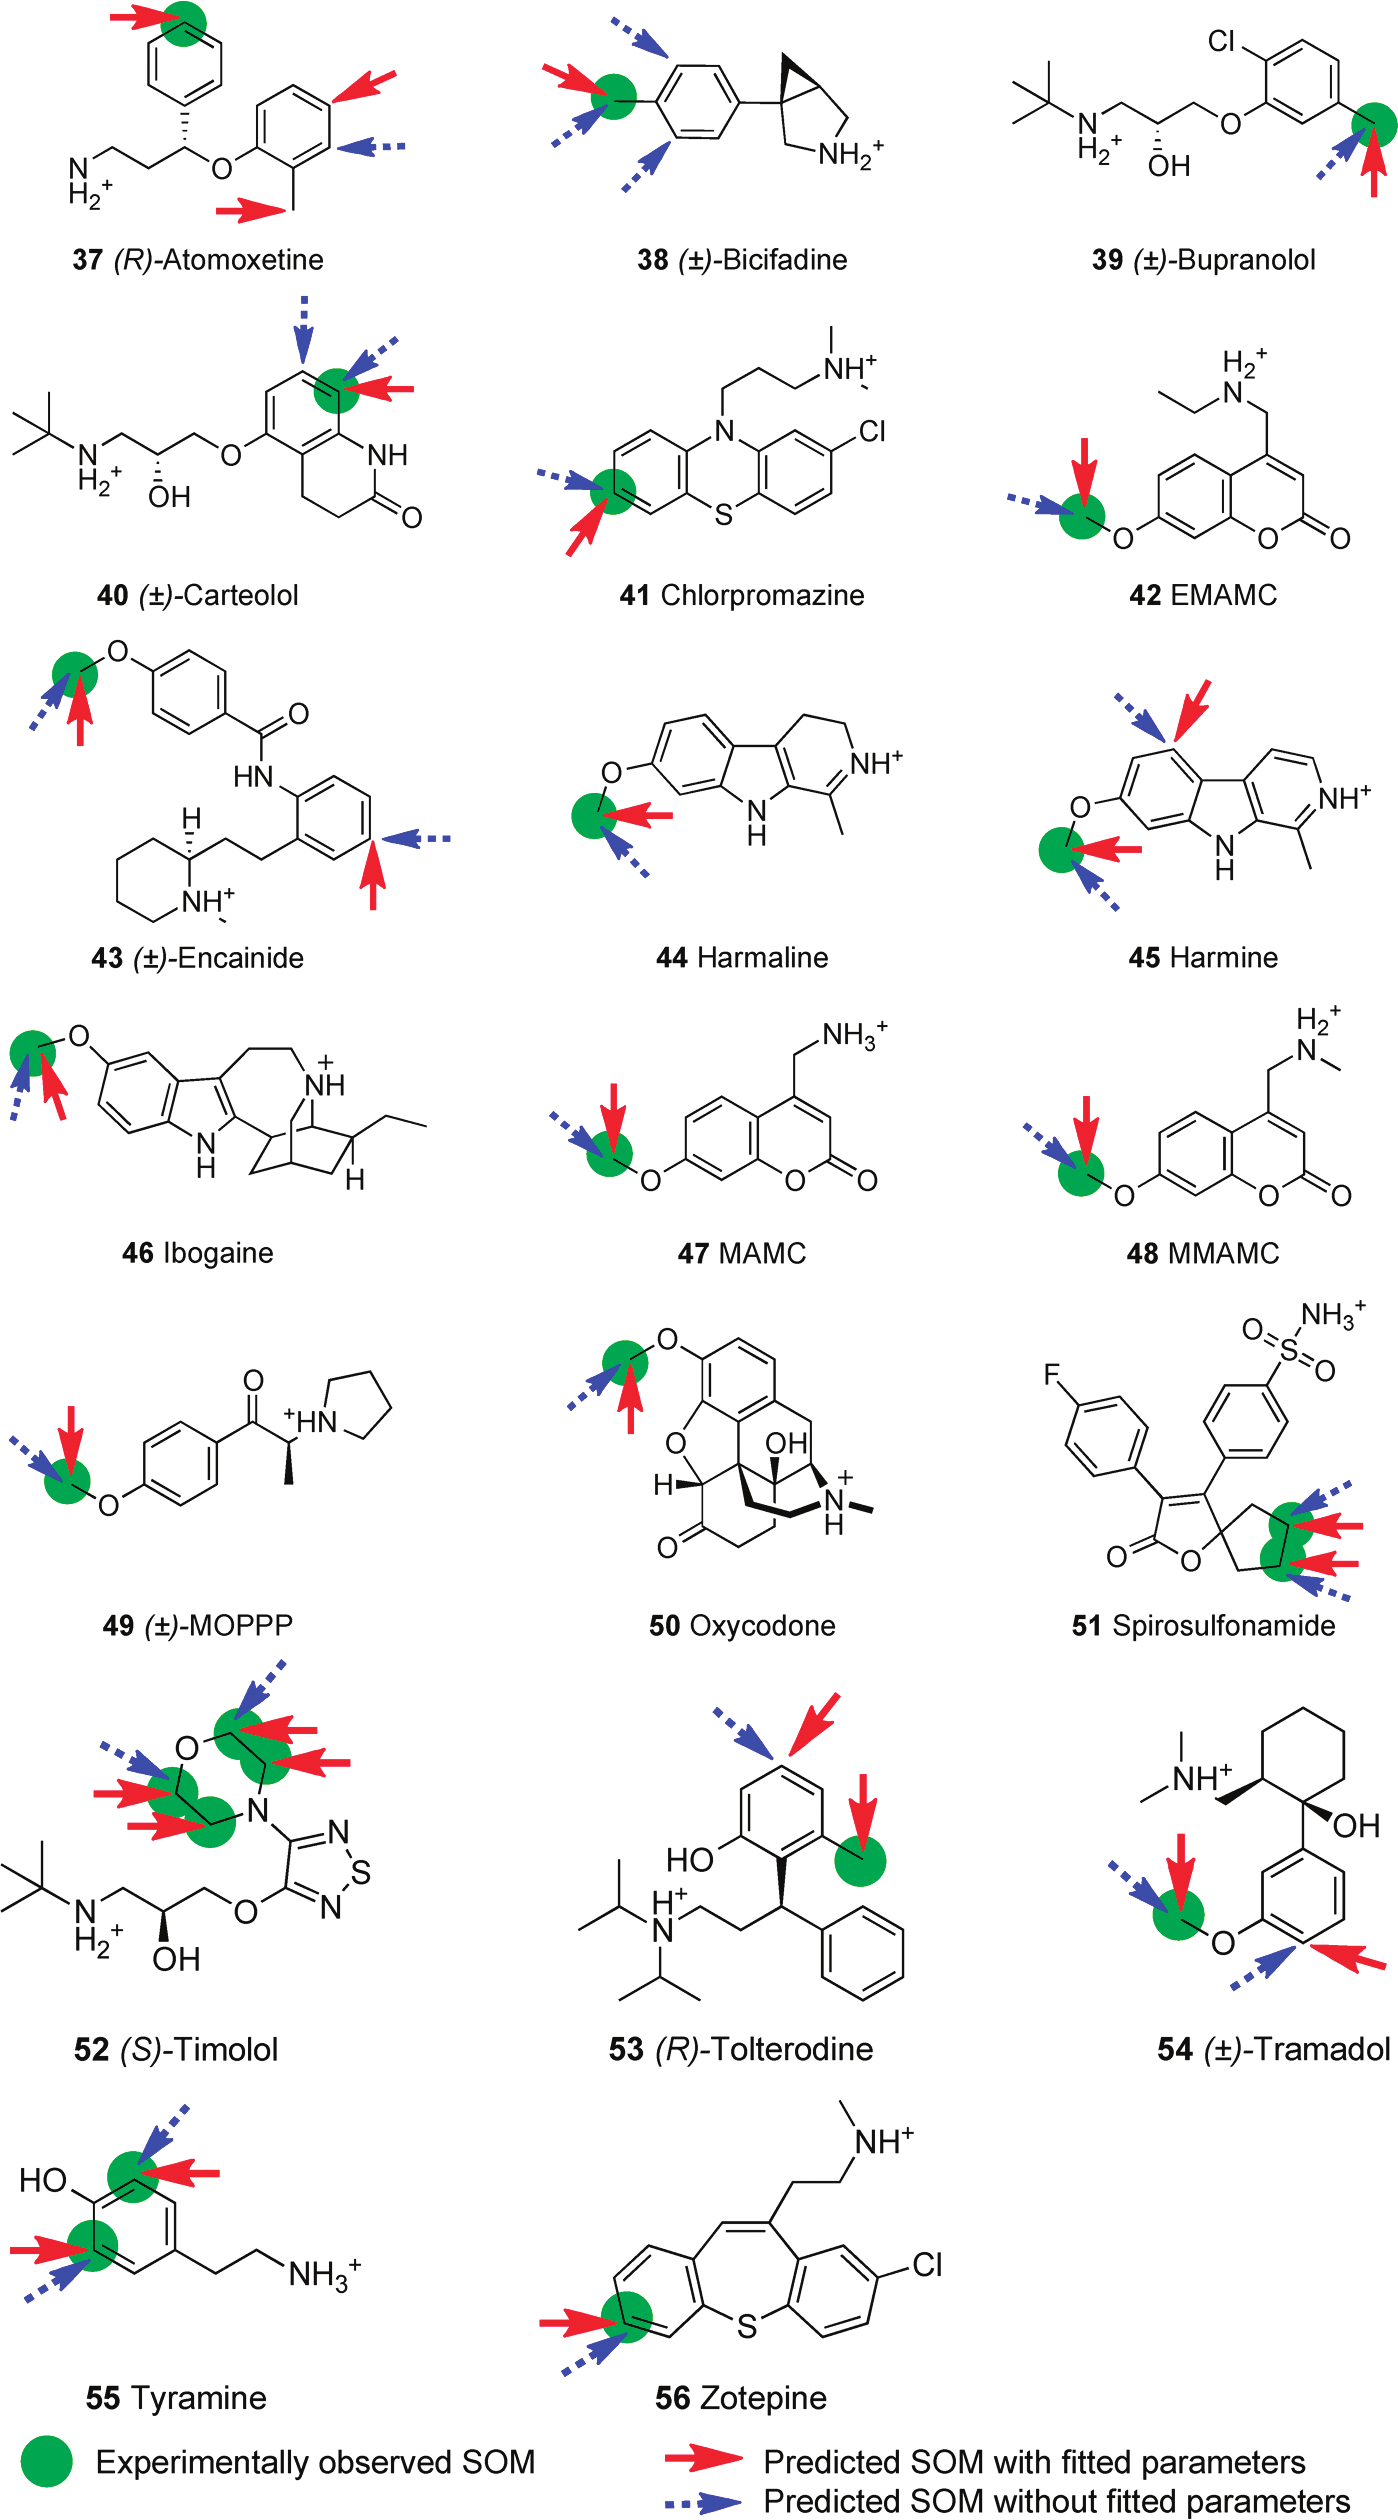
\includegraphics[width=0.65\textwidth]{figures/idsite/idsite_figure-009.png}
\caption{Physical and fitted IDSite predictions of sites of metabolism on the test set.}
\label{fig:idsite_test}
\end{figure}


\section{Discussion}
\label{section:p450/discussion}


\chapter[p450 Sites of Metabolism]{Prediction of p450 Sites of Metabolism}
\section{Introduction}
\label{section:p450/introduction}
The most common method of drug clearance among currently perscribed drugs is metabolism, which is the primary method of clearance for approximately 75\% of the top 200 most commonly perscribed drugs in the United States \cite{williams2004drug}.
Cytochrome p450 is critical to drug metabolism, being active in approximately 75\% of drugs which are cleared in this method \cite{guengerich2007cytochrome}.

\begin{figure}[h]
\centering
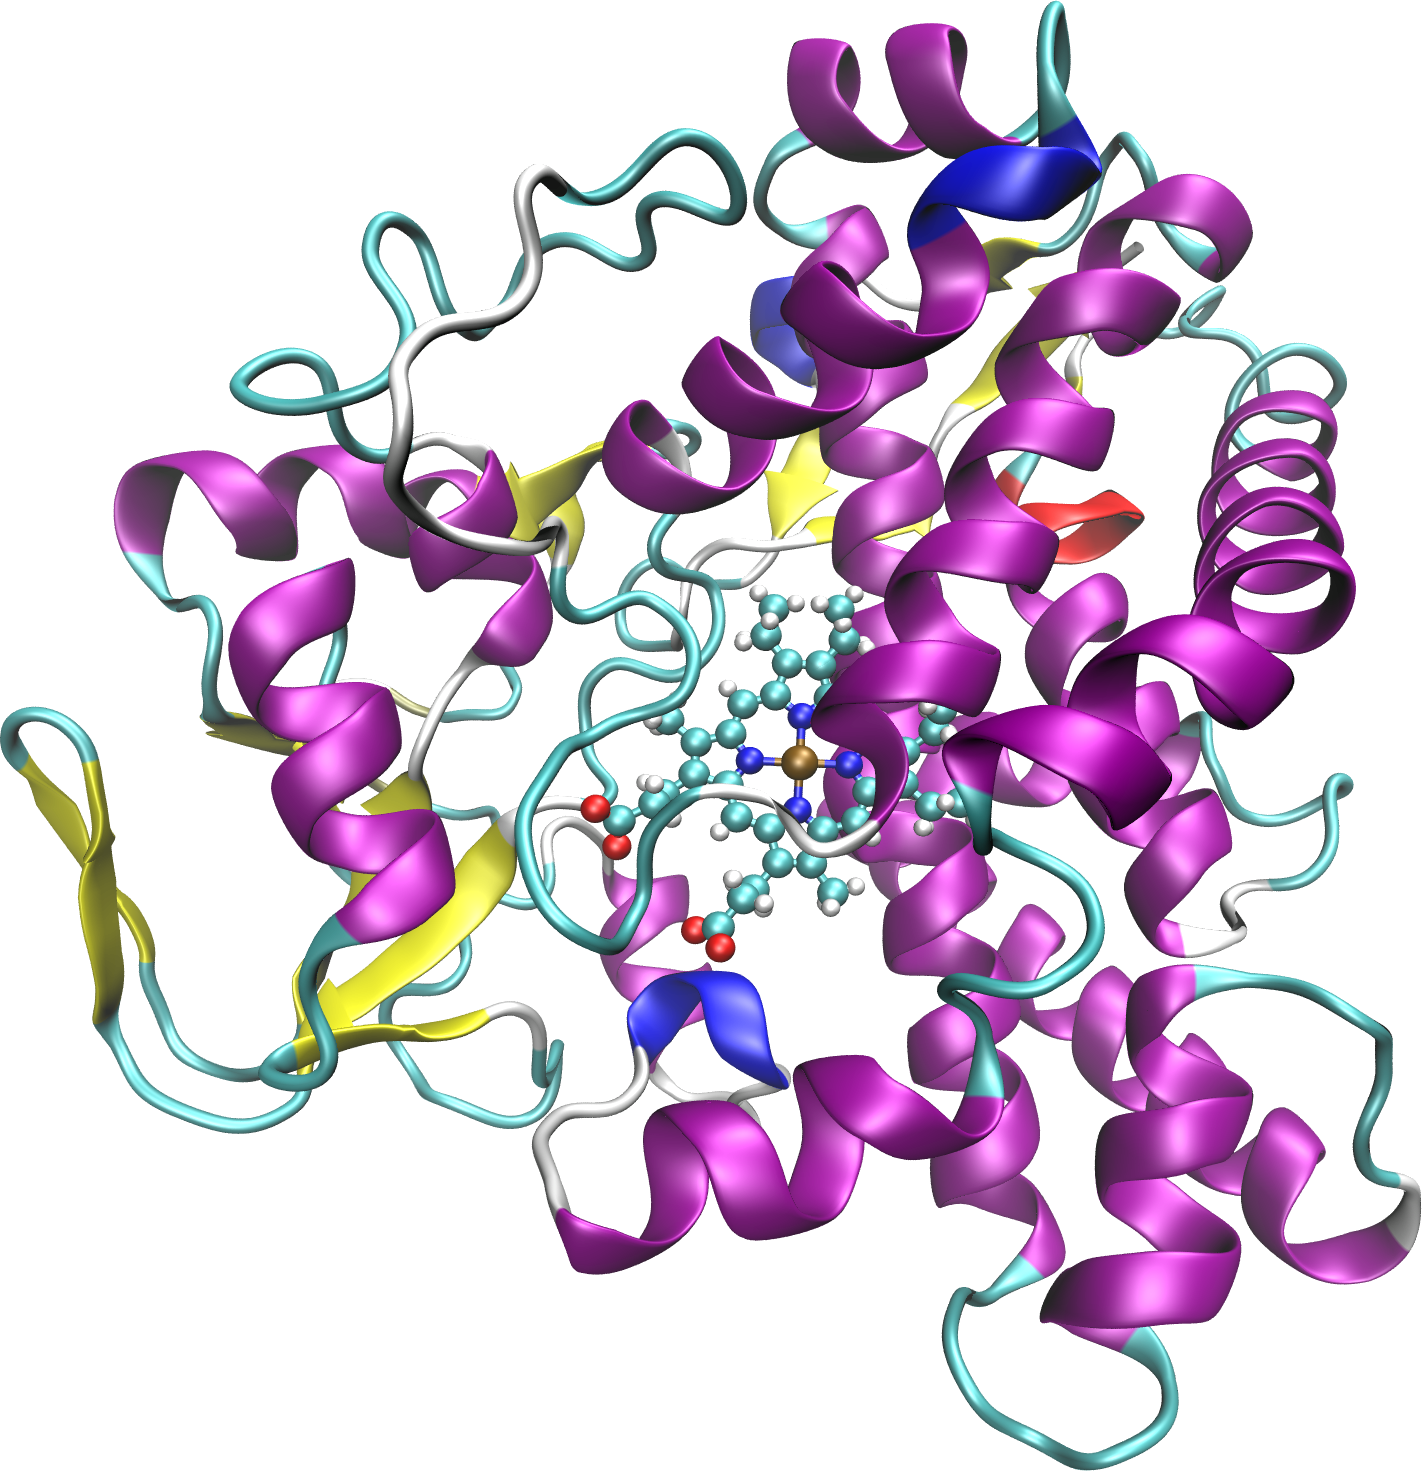
\includegraphics[width=0.5\textwidth]{figures/p450.png}
\caption{
The structure of cytochrome P450, taken from PDBid 1JFB, shown in cartoon representation.
The bonded heme group, shown as ball and stick model, is visible in the center.
}
\label{fig:p450}
\end{figure}


\section{Methods}
\label{section:p450/methods}

\begin{figure}[h!]
\centering
\includegraphics[width=0.55\textwidth]{dot_files/idsite.png}
\caption{An overview of the entire IDSite procedure.
The dotted lines represent abbreviated versions of the full procedure.
Receiver operating characteristic graphs for the full version, and these abbreviated versions, are presented in \ref{figure:idsite_roc_sampling}.
Series colors on ROC graphs correspond to arrow colors here.}
\label{figure:idsite_overview}
\end{figure}

Prediction of sites of metabolism is a three stage procedure:
\begin{enumerate}
\item Initially a number of different ligand conformations are generated, and these are docked into a rigid protein, with soft VDW terms using Glide \cite{halgren2004glide,friesner2004glide}.
\item The docked conformations are refined using a Monte Carlo Minimization (MMC) approach which samples degrees of freedom in both the ligand and protein.
\item Refined conformations are classified into reactive site or non-reactive site on the basis of the energy of the refined conformations and the intrinsic reactivity of the site. \cite{li2011idsite}
\end{enumerate}

\subsection{Docking}
\label{subsection:p450/docking}
In the initial docking stage of the IDSite protocol Glide is used to generate a number of proposed docked conformations for each ligand.
Glide (standard precision) is used to generate a number of different ligand conformations by sampling conformations of freely rotatable bonds and rings.
A bounding box, which will be used for a grid search, is defined centered at the centroid of the ligand with an edge length of 10 angstroms.
Because the crystal structure used for CYP2D6 (PDBID: 2F9Q) does not have a ligand, the centroid of residues Glu216, Asp301, Thr309, and Phe483 was used instead in this case.
Because the steric clashes present in many proposed docked conformations can be relieved using a simple minimization procedure a reduced Van der Waals (VDW) radii are used in the docking stage for non-polar atoms.
The VDW radii used for the P450 are scaled by a factor of 0.4, and the scaling for the ligand starts at 0.8.
If an insufficient number of poses, in this case fewer than four, are found using these scaling factors for the radii the scaling of the ligand is stepped down until at least four poses are found.
Additional filtering of possible high energy conformations was also skipped in order to ensure the greatest diversity of docked poses reached the refinement stage.
The collection of docked poses are then clustered according to the RMSD of the ligand, and each pose is minimized.
The top sixty ranked poses according to the Glide SP metric are retained screened using a number of different criteria.
A hard sphere overlap criteria is used to remove poses with obvious steric clashes which were not removed during the minimization procedure.
A conserved feature of CYP2D6 ligand complexes is a salt bridge with Glu216 or Asp301.
In order to reduce sampling cost IDSite only considers structures with at least one hydrogen-bond donor within 4 residues of the centroid of these two residues and Ser304.
The sphere defined by these residues is illustrated along with the bounding box used for sampling in Figure \ref{fig:idsite_glide}
A number of other rule based geometric screens are used to remove structures which are unlikely to react.
Structures meeting any of the following criteria:
\begin{enumerate}
\item The distance of the basic nitrogen to the ferryl oxygen is less than 5.0 angstroms;
\item The distance of the basic nitrogen to the negative charged oxygen (in Glu216 or Asp301) is greater than 5.5 angstroms;
\item More than 2 heavy atoms from the ligands are further than 16.0 angstroms away from the heme iron;
\item More than 1 heavy atom from the ligand are closer than 1.0 angstroms to the receptor;
\item More than 6 heavy atoms from the ligand are closer than 1.8 angstroms to the receptor;
\item No heavy atom in the ligand is within 5.0 angstroms to the heme iron;
\end{enumerate}
are removed.
If the number of structures at this point is too low, the VDW scaling factors of the non-polar atoms of the ligand are stepped down, and the process is repeated.
If four or more poses are found at these point these poses are passed onto the next stage of the IDSite procedure, the Monte Carlo Minimization refinement stage.

\begin{figure}[h]
\centering
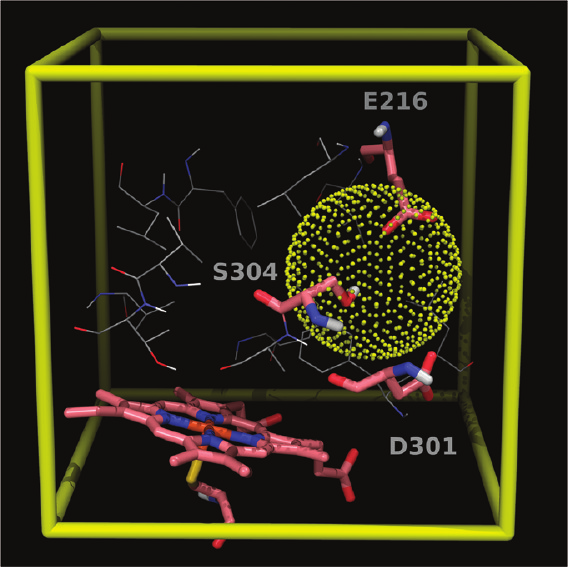
\includegraphics[width=0.35\textwidth]{figures/idsite/glide.png}
\caption{An overview of the entire IDSite procedure.}
\label{fig:idsite_glide}
\end{figure}

% IDSite uses reduced VDW radii for nonpolar atoms both in the protein receptor and the ligand, so that slight steric clashes are tolerated during the docking stage.
% For the protein receptor the VDW scaling factor is fixed at 0.40, while for the ligand, the scaling factor starting from 0.80 is adaptively adjusted until at least 4 valid poses are found.
% With highly flexible ligands and relatively high scaling factors, Glide often finds only a handful of valid poses, and even fewer survive after IDSite screening.
% However, if the scaling factor is set too low, the docked poses may contain too many serious steric clashes, which can cause problems in the subsequent minimization.
% If IDSite fails to find enough valid poses, the scaling factor is adjusted and the number of poses to pass the initial docking phase in Glide is increased accordingly to augment sampling.

% joe is this far
% If the ligand contains other hydrogen-bond donors except for the basic nitrogen, the constrained docking is likely to generate poses that form hydrogen bonds instead of the salt bridge to Glu216 or Asp301.
% However, IDSite is able to distinguish these poses and filter them via an additional salt bridge filter in the pose screening, so that only the poses with a stable salt bridge are allowed to pass to the refinement stage.


\subsection{Monte Carlo Minimization Refinement}
\label{subsection:p450/mcm}
Since the emphasis in IDSite sampling is efficient sampling of low energy conformations, as only the lowest energy conformations are passed on to the next stage of prediction, Monte Carlo Minimization was used instead of a more traditional Monte Carlo simulation because it provides more efficient sampling of low energy conformations (see \ref{subsection:monte_carlo}).
The Monte Carlo Minimization sampling used by IDSite for refinement incorporates three different types of steps: side chain motions, rigid body transformations, and hybrid Monte Carlo simulations.
For each Monte Carlo step, one of three types of motions is selected according to the weighted probabilities, which are different for the two different PLOP sampling stages (see table \ref{table:mmc_params}).
\begin{table}[h]
    \centering
    \begin{tabular}{|c|c|c|}
        \cline{2-3}
        \multicolumn{1}{r|}{~}                       & \multicolumn{2}{c|}{PLOP Sampling Stage} \\
        \cline{2-3}
        \multicolumn{1}{r|}{~}                       & First                        & Second                        \\
        \hline
        Number of Residues Sampled                   & 12                           & 40                            \\
        \vspace{-1.5ex}
        Number of Structures                         & \multirow{2}{*}{max(n*8,24)} & \multirow{2}{*}{max(n*20,60)} \\
        Advanced to Next Stage                       &                              &                               \\
        P(side chain step)                           & 0.5                          & 0.7                           \\
        P(rigid body step)                           & 0.1                          & 0.2                           \\
        P(HMC)                                       & 0.4                          & 0.2                           \\
        \hline
    \end{tabular}
    \caption{The number of residues sampled as well as the number of structures advanced to the next stage from each of the sampling stages.
Also, the relative probabilities of selecting each of the different sampling steps during a Monte Carlo minimization sampling stage.}
    \label{table:mmc_params}
\end{table}

Using the chosen method, a new conformation is proposed and minimized before the Metropolis acceptance criteria (equation \ref{equation:metropolis_acceptance}) is applied to the proposed state, using a temperature of 300 K.
All atoms of all residues with any atom within 5 angstroms of the ligand in the starting crystal structure were allowed to move during Monte Carlo moves, including the ligand itself.

During the minimization Monte Carlo sampling stages of the IDSite procedure, artificial constraints are used to guide the sampling towards a transition state like conformation.
These constraints create artificial bond or angle potentials, which affect the minimization but are not used in the Monte Carlo acceptance test.
For each of the minimization Monte Carlo sampling stages of the IDSite procedure, two different sets of constraints are applied depending on the hybridization of the carbon atom at the possible site of metabolism, for a total of four possible different sets of constraints.
In the first minimization Monte Carlo stage, two constraints are applied, shown in figures \ref{figure:first_sp2_constraints} and \ref{figure:first_sp3_constraints}:
\begin{enumerate}
\item The sulfur-iron-carbon angle is constrained to 145 degrees, with 20 degrees of ``slack'', or a flat bottom to the potential well (denoted as 145\plusorminus20 degrees).
The spring constant of this constraint is about 25 kcal/mol/degree\superscript{2}, or {\textapprox}40\% the strength of a carbon-carbon-carbon angle.
\item A ``dummy'' oxygen atom is placed above the plane of the heme group, in the same position that it would occupy if an oxygen molecule was bound to the heme.  
This dummy atom has no interactions with other atoms, but is used as the anchor of a distance constraint for the carbon at the site of metabolism.  
The carbon-dummy oxygen distance is constrained to 2.5\plusorminus0.5 angstroms.
The spring constant of this constraint is 100 kcal/mol/angstrom\superscript{2}, approximately 1/3rd the strength of a carbon-carbon bond.
\end{enumerate}
\begin{figure}
\centering
\begin{subfigure}[b]{0.35\textwidth}
\centering
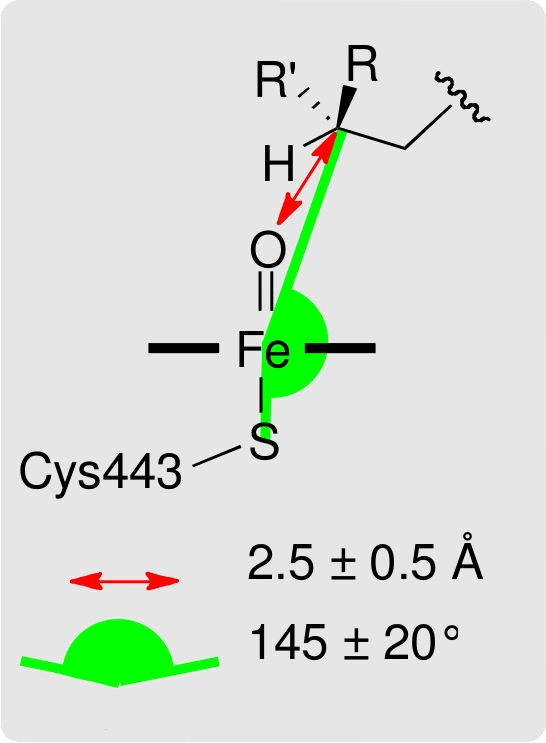
\includegraphics[width=\textwidth]{figures/idsite/33a}
\caption{}
\label{figure:first_sp3_constraints}
\end{subfigure}
\hspace{0.1\textwidth}
\begin{subfigure}[b]{0.35\textwidth}
\centering
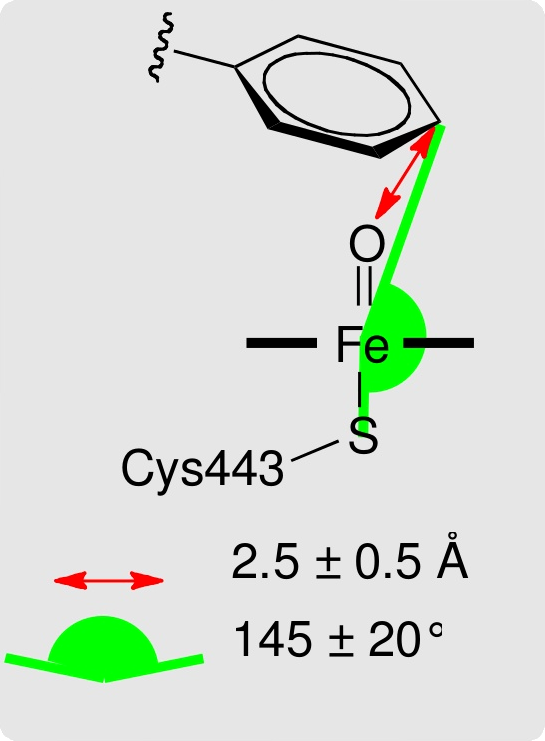
\includegraphics[width=\textwidth]{figures/idsite/33b}
\caption{}
\label{figure:first_sp2_constraints}
\end{subfigure}
\caption{The constraints applied to (a) sp\superscript{3} and (b) sp\superscript{2} atoms during the constrained minimization and first minimization Monte Carlo sampling stage.
The spring constant of the bond constraint (red arrow) is 100 kcal/mol/angstrom\superscript{2}, and that of the angle constraint is 25 kcal/mol/degree\superscript{2}.
The oxygen atom depicted in this figure is a ``dummy'' atom and does not interact with any other atoms in the structure except through the constraint.}
\label{figure:first_constraints}
\end{figure}


In the second minimization Monte Carlo sampling stage, the constraints are different for sp\superscript{2} and sp\superscript{3} carbons.
These constraints are illustrated in figures \ref{figure:second_sp3_constraints} and \ref{figure:second_sp2_constraints}.
For sp\superscript{3} sites:
\begin{enumerate}
\item the hydrogen bound to the carbon at the possible site of metabolism is constrained to a distance of 1.25\plusorminus0.1 angstroms and a spring constant of 20 kcal/mol/angstrom\superscript{2},
\item the carbon in question is constrained to 2.2\plusorminus0.8 angstroms and a spring constant of 10 kcal/mol/angstrom\superscript{2},
\item the heme iron-hydrogen-carbon angle is constrained to 138\plusorminus5 degrees and a spring constant of 20 kcal/mol/degree\superscript{2}.
\end{enumerate}
For sp\superscript{2} sites:
\begin{enumerate}
\item the carbon at the possible site of metabolism is constrained to 1.8\plusorminus0.1 angstroms and a spring constant of 20 kcal/mol/angstrom\superscript{2},
\item both adjacent carbons are also constrained to the dummy oxygen atom, at a distance of 2.5\plusorminus0.1 angstroms and a spring constant of 20 kcal/mol/angstrom\superscript{2}, and
\item finally, the hydrogen bonded to the carbon at the possible site of metabolism is constrained to the oxygen atom at a distance of 2.0\plusorminus0.1 angstroms and a 20 kcal/mol/angstrom\superscript{2} spring constant.
\end{enumerate}
\begin{figure}
    \centering
    \begin{subfigure}[b]{0.35\textwidth}
    \centering
    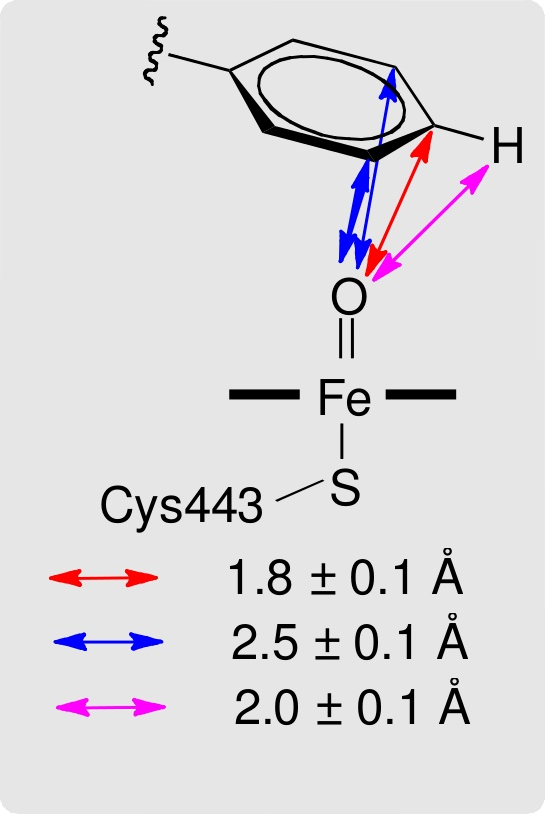
\includegraphics[width=1.0\textwidth]{figures/idsite/34b}
    \caption{}
    \label{figure:second_sp2_constraints}
    \end{subfigure}
    \hspace{0.1\textwidth}
    \begin{subfigure}[b]{0.35\textwidth}
    \centering
    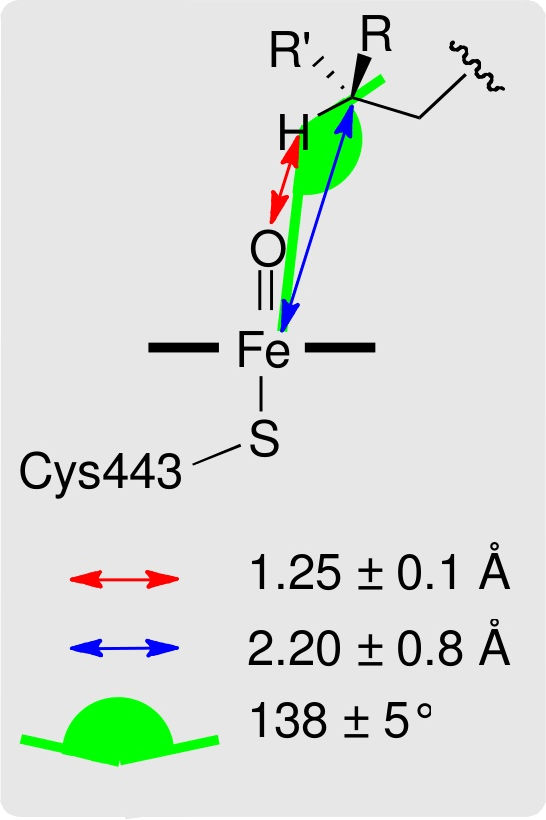
\includegraphics[width=1.0\textwidth]{figures/idsite/34a}
    \caption{}
    \label{figure:second_sp3_constraints}
    \end{subfigure}
    \caption{The constraints applied to (a) sp\superscript{2} and (b) sp\superscript{3} atoms during the constrained minimization and second minimization Monte Carlo sampling stage.}
    \label{figure:second_constraints}
\end{figure}
 

As CYP2D6 forms a conserved salt bridge with the substrate with either glutamate 216 or aspartate 301 \cite{paine2003residues}, this was also incorporated as a constraint during the sampling stages.
In the first sampling stage, this salt bridge is enforced by introducing a harmonic constraint of 3.0\plusorminus0.3 angstroms between the basic nitrogen of the substrate and each of the side chain oxygen atoms in GLU216, ASP301, and SER304 (see figure \ref{figure:salt_bridge_first}).
The spring constants of these constraints are 15.0, 8.0, and 4.0 kcal/mol/angstrom\superscript{2} for GLU216, ASP301, and SER304, respectively.
Additionally, an angle constraint of 150.0\plusorminus30.0 degrees with spring constant of 5.0 kcal/mol/degree\superscript{2} is applied to each of the N-H-O angles.
\begin{figure}[hp]
\centering
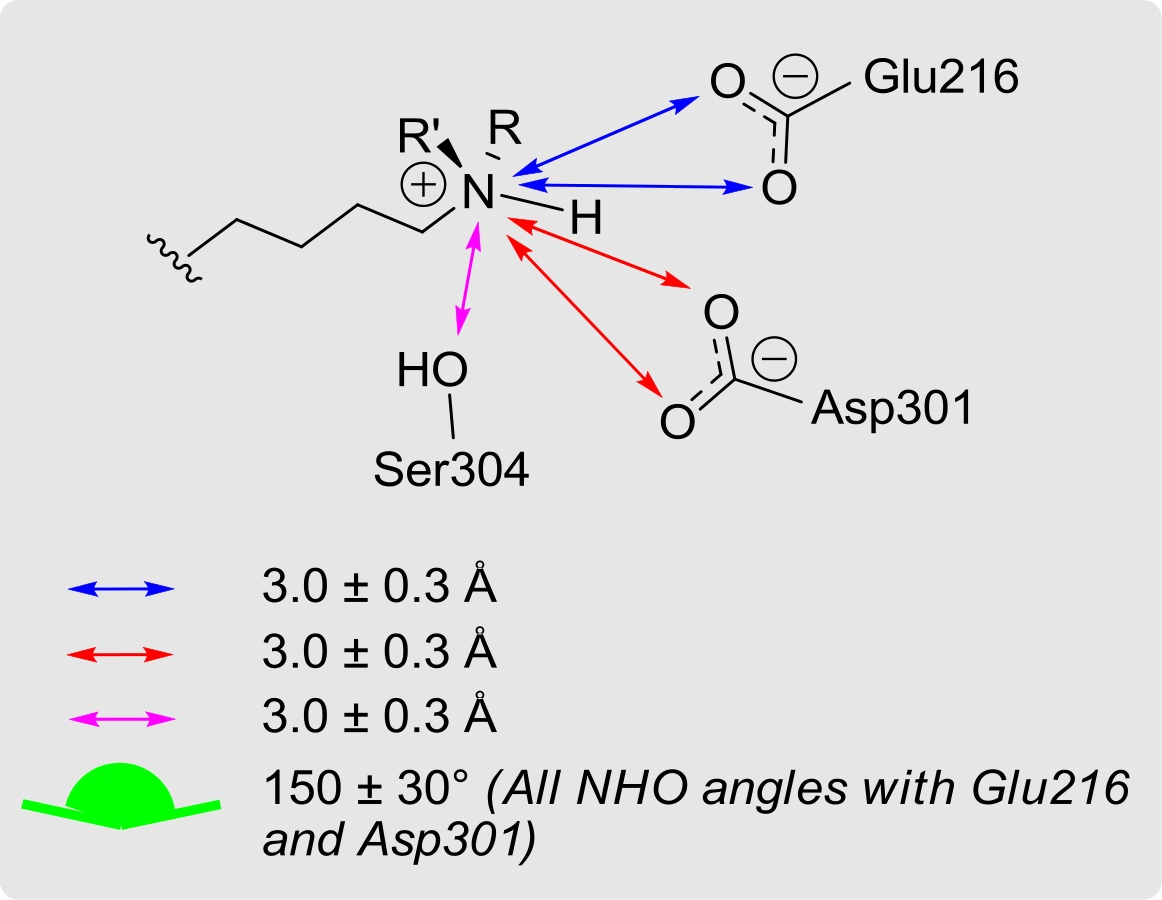
\includegraphics[width=0.50\textwidth]{figures/idsite/salt_bridge_first}
\caption{The constraints applied to the salt bridge region of CYP2D6 during the {\it first} minimization Monte Carlo sampling stage.}
\label{figure:salt_bridge_first}
\end{figure}

In the second sampling stage, four separate trajectories are calculated for each of the four carboxalate oxygens of GLU216, ASP301 (shown in figure \ref{figure:salt_bridge_second}).
In each trajectory a constraint of 1.9\plusorminus0.1 angstroms is applied between the hydrogen attached to the basic substrate nitrogen and one of the four carboxalate oxygens.
Additionally, the angle of the hydrogen bond is constrained to 168\plusorminus12 degrees, with a spring constant of 5.0 kcal/mol/degree\superscript{2}.
\begin{figure}[hp]
\centering
\includegraphics[width=0.50\textwidth]{figures/idsite/salt_bridge_second}
\caption{The constraints applied to the salt bridge region of CYP2D6 during the {\it second} minimization Monte Carlo sampling stage.}
\label{figure:salt_bridge_second}
\end{figure}
 % figure

\begin{figure}[hp]
\centering
\includegraphics[width=0.7\textwidth]{dot_files/mcm_flowchart.png}
\caption{An outline of the Monte Carlo minimization refinement stages in PLOP.}
\label{figure:mcm_flowchart}
\end{figure}

Three different methods of sampling, or moves, were implemented in order to sample different protein-ligand conformations.
A flow chart presenting the minimization Monte Carlo procedure is presented in figure \ref{figure:mcm_flowchart}.
\begin{enumerate}
\item Side chain moves.
Several types of side chain motions were implemented in PLOP.
In all cases, they are defined in a such a way that they can be applied to both ligands and proteins.
The same atomic overlap screening function implemented with the rigid body Monte Carlo was implemented with the side chain torsional moves.
a. Random torsion angle moves: The first type of move that was implemented is random movement of torsional chi angles.
For small torsion moves, a random perturbation of the angle of +/- X is made, where X is a random number with user defined magnitude.
For large torsion moves, for each torsion angle that is changed, a random angle is selected in the form 60*Y +/- X, where Y = 1 through 5, and X is the same random number for the small torsion moves.
The large move was introduced since positions at the top of rotamer barriers are relatively unlikely to be selected, and efficiency thus can be improved by focusing on the more probable moves.
The ratio of small to large torsion moves can be used-adjusted, as can the ratio of probabilities of changing all the torsions in a randomly selected side chain versus changing only one single (randomly selected) torsion among all the free torsions in the simulation can be set as a user-defined parameter.
Rotamer side chain moves: A second type of torsional samples implemented is random selection of a new rotamer state for the entire side chain, plus an optional user defined small noise term for each torsion in the rotamer state.
A database of protein rotamer states obtained from crystallographic data are already a part of PLOP \cite{xiang2001extending} Rotamer libraries for ligands are generated by examining all possible side chain conformations at 10 degree resolution and screening this set for steric clashes.
A Monte Carlo move in this case represents a choice of a new torsional rotamer state for the entire side chain.
Monte Carlo moves based on torsional states cannot lead to correct equilibrium distributions, as transitions from non-rotamer states to rotamer states are defined, but not reverse transitions, upsetting detailed balance.
However, a pretabulated rotamer state is more likely to be low energy than a randomly generated torsional state, and thus allows for more diverse conformational searching.
Correlated torsional moves: Most torsional rearrangements of the side chains in the core of proteins are highly correlated because of the density.
In order to attempt to include correlated torsional motion, at each step we examine the distance between all pairs of beta carbons in the ligands that are free to move.
At each step, for the set of side chains that are free to move, clusters where beta carbons are all mutually within a user-specified distance are identified.
This process takes a trivial amount of time compared to an energy evaluation, so does not slow the simulation at all.
Then, with user specified probabilities, clusters of different sizes are selected for the torsional moves, either with random side chain moves, or rotamer selection moves.
By selecting only clusters where all residues are mutual neighbors, detailed balanced is observed for simulations where accurate equilibrium sampling is desired.
By varying the dihedral angles of the rotatable bonds, IDSite uses side chain MC moves in PLOP to sample the selected side-chain conformations of the protein and of the ligand.
Up to three close residues (C beta distance within 6 angstroms) are allowed to rotate collectively, but the moves of the protein residues and those of the ligand are separated.
In each attempted movement, the conformations of the selected side chains (from the protein/ligand) are either changed by random perturbations or assigned by the randomly selected rotamers from a library.
For an attempt with a random perturbation, the displacement of each dihedral angle is the sum of a large rotation (N times 60 degrees with N as a random integer between 0 and 5) and a random perturbation from 0 to 30 degrees.
For a rotamer library attempt, a side-chain conformation is updated with a random rotamer from a high resolution side-chain library for protein residues \cite{xiang2001extending}, and from a homogeneous library at 10 degree resolution for the ligand.
If a structure with tolerable overlaps is generated in an attempt, it is minimized and sent to subsequent stages for judgment of acceptance.
Each side-chain move takes less than 15 seconds and is the fastest among all the three move types.

% from mike's
For side chain Monte Carlo, a steric screen with an overlap factor of 0.6 was used.
Rotamer torsional moves were selected 75\% of the time, with half of the remaining being of random torsions, and the other half random perturbations of all torsions within the randomly selected side chains.
Clusters of size 1 (i.e. single side chains), size 2 and size three were selected in equal proportion, and all side chains in the cluster were perturbed with the selected torsion move.
A mutual beta carbon distance of 6 Angstroms was used for the clustering size.
Small torsion perturbations made +/- 60 degress from the current dihedral angle, and were performed 5\% of the time; Large periodic moves were performed 95\% of the time.
Only outer steps were performed, and each side chain Monte Carlo series consisted in only one move.
Minimization was performed after the single step, and acceptance was performed at 1 K.


\item % TODO
Rigid motion moves.
Rigid body translation and rotation were also implemented for noncovalently linked moieties, such as ligands.
Random rotations and translations were coupled together, allowing for more concerted movement.
Rigid body move implemented in PLOP can optionally include a screening step, where atomic Lennard-Jones overlaps that would lead to energies much higher than would be observed in any conceivably long equilibrium simulation are rejected without further evaluation.
A ratio of 0.7 between the distance between the two atoms and the sum of the Lennard-Jones radii of the two atoms yields energies on the order of 10's of thousands of kcal/mol, and is thus reasonable to maintain equilibrium sampling in a Monte Carlo simulation.
Translations were implemented in a random direction, with a user-defined magnitude.
Rotations were implemented by picking a random quarternion (a random angle around a random axis, through the geometric center of the rigid group) with a user specified maximum random angle centered around either the current angle, or 180 from the current angle, in the case of a flip.
Multiple time scale Monte Carlo sampling was also implemented with rigid body moves, with short range and long range interactions defined as above.
In addition, an option to compute the inner Monte Carlo loops with reduced Lennard-Jones radii were also implemented, to increase the ability to escape from tight spacial bottlenecks.
In this case, the long time step energies are the full energies with unscaled Lennard-Jones radii.
This increases the conformational freedom and therefore sampling for the short, at a cost of decreasing the acceptance probability in the outer loop.
Scaled Lennard-Jones radii were also implemented in multiple time dynamics, but yielded very little apparent improvement because of the lack of phase space overlap between dynamics with different scaled Lennard-Jones radii).
Rigid body moves are used to sample the translational and rotational space of the ligand.
Multiple attempts with reduced VDW radii are applied, as it is quite common to fail in searching for a clash-free conformation in a single rigid body moving attempt (especially when the ligand is large and flexible and the binding pocket is relatively small).
Each rigid body move includes 1000 attempts, and each attempt performs a translation along a random vector and a rotation around a random axis, with less than 0.5 angstroms and 60 degree displacement, respectively.
In addition, the VDW radii are reduced (scaling factor 0.8) to soften the Lennard-Jones potential, so that mild steric clashes are allowed, which are likely to be resolved by the subsequent minimization.
The rigid body move usually takes 20 to 40 seconds per move.

% from mike's
For rigid body Monte Carlo, a steric screen with an overlap factor of 0.7 was used, with a translation size of 0.5 Angstroms and a rotation size of plus or minus 60 degrees.
No flip moves were included, as flips were not anticipated with the geometry of the ligand system [Robert, check this is true?] A Lennard-Jones scaling parameter of 0.8 was used during the inner steps.
Each rigid MC step consisted of 1000 inner steps, and only one outer step, meaning that only one minimization occurred each time rigid body Monte Carlo was selected as the move step.


\item The Hybrid Monte Carlo (HMC) \cite{duane1987hybrid} step is a velocity verlet molecular dynamics simulation.
This simulation allows all atoms in both the ligand and residues containing atoms withing 5 angstroms of the ligand to move.
Initial velocities are taken from a Maxwell-Boltzmann distribution at 900 K.
Bonded and short range interactions evaluated every 1 nanosecond inner time step, and long range potentials are assumed to be fixed over inner steps.
Five inner steps compose each outer HMC step.
In the outer step the molecular surface, long range interactions and, Born alphas are updated before computing the energy and applying the Metropolis acceptance criteria at a temperature of 900 K after each MD run.
Taking up to 15 minutes per move, the HMC is the most expensive among all three types of moves in PLOP.

%, with long range interactions evaluated every long time step.
%In this case, molecular dynamics is run only using only the short range energies, which will conserve energy and thus yield proper Markov chain behavior while the cutoffs and Born alpha are not updated.
%Inner loop Monte Carlo steps are performed with only the short range dynamics, and outer loop Monte Carlo steps are performed with all interactions.
%In the case of implicit solvent simulations, the Born alpha are only reevaluated in the outer loop Monte Carlo steps.
%This allows for evaluation of the full surface integral relatively infrequently, and yields a properly weighted Boltzmann distribution of conformations without needing position derivatives of the Born alphas.

%Energies are conserved in vacuum simulations if the long range cutoff extends to cover the entire molecule.
%With implicit solvent dynamics, energies are not conserved as there is no derivative of the Born alpha with respect to position, so a thermostat must be used to approximate realistic dynamics.
%One mode of action is to run HMC on top of normal RESPA dynamics, with acceptance and rejections done after a fixed number of steps of MD, as in typical HMC.
%Velocities are re-randomized after every Monte Carlo step from the Maxwell-Boltzmann distribution.
%However, HMC can also be implemented in a multiple-time step Monte Carlo framework \cite{hetenyi2002multiple}.
%The hybrid Monte Carlo (HMC)\cite{duane1987hybrid} move in PLOP performs simultaneous sampling for the selected residues in the protein side chains and backbone as well as the ligand.
%Each HMC move performs a 5 picosecond, constant energy molecular dynamic (MD) simulation (starting at 900K) on all the atoms in the selected residues.
%Taking up to 15 minutes per move, the HMC is the most expensive among all three types of moves in PLOP.

%The underlying molecular dynamics for the hybrid Monte Carlo consisted of 500 5 ns RESPA \cite{tuckerman1991molecular} steps, each with 5 1 ns short range steps.
%The dynamics were initialized from a Maxwell-Boltzmann distribution at 900 K, and then run without any thermostat the full 2.5 ps run.
%Minimization was performed after the single HMC step, with acceptance/rejection performed at a Monte Carlo temperature of 900 K.

% is built on top of a molecular dynamics (MD) integrator.
% We implemented velocity verlet MD using the RESPA formalism \cite{tuckerman1991molecular}, with bonded and short range interactions evaluated every inner time step, with long range interactions evaluated every long time step.
% We also included in the including Andersen, Berendsen, and Langevin thermostats, as well as Brownian Dynamics.
% Short range interactions included all bonded interactions and nonbonded interactions less than a user-specified cutoff.
% Both short and long range cutoffs are dipole-based as described in a previous paper [cite].
% and then run without any thermostat the full 2.5 ps run.

\end{enumerate}

\subsection{Evaluation}
\label{subsection:p450/evaluation}
Both a parameterized and an unparameterized model were used to classify potential sites of metabolism.
IDSite makes the assumptions that all intermediates before the rate determining step are at equilibrium \cite{wang2007stochastic}, that hydrogen abstraction is the rate limiting step for hydroxilation of aliphatic carbons and electrophilic attack is the rate limiting step for hydroxilation of aromatic rings \cite{guengerich2001common,shaik2005theoretical}.
With these assumptions the rate of metabolism at each possible site of reaction is affected by the free energy of binding in order to put that site in the site of reaction, as well as the free energy barrier of rate determining step, or
\input{equations/curtin_hammett} % dG = dG bind + dG react
The ${\Delta}G_{\mathrm{binding}}$ above is calculated using a PLOP evaluation of the refined pose.
The intrinsic reactivity for the system is computed from DFT calculations on a simplified system, replacing the heme with a methody radical, and using a linear relationship between $IR(\mathrm{heme})$ and $IR(\mathrm{methoxy\ radical})$ to estimate the true reactivity for the heme system.
\begin{figure}[h]
\centering
\includegraphics[width=0.8\textwidth]{figures/idsite/intrinsic_corrected.png}
\label{fig:idsite/intrinsic}
\caption{The linear relationship between the calculated intrinsic reactivity of the methoxy radical complex and that of the heme complex.
Adapted from \protect\cite{li2011idsite} with minor correction.
In the original manuscript the slope of the regression was reported as 1.117 and that number was used throughout.
This difference should not significantly affect the physical IDSite classifier results, and does not affect the results of the fit model.
In the rest of this text the value from the original publication of 1.117 will be used.}
\end{figure}
\input{tables/heme_methoxy.tex}
\input{equations/intrinsic_reactivity} % estimate from abbreviated reactivity
Since this constant $C$ is identical for each state it has no effect on the relative differences in ${\Delta}G_{\mathrm{site}}$ or the relative rate of metabolism at possible sites.
\input{equations/g_site} % E/G equation
Since the ligand is forced to assume a different conformation in order to react, the energy of this transition state conformation, $E_{\mathrm{TS}}$, is also computed using PLOP.
As the relative abundance of different metabolites is determined by differences in ${\Delta}G$ per site rather than absolute reactivities, the constant in equation \ref{equation:g_site} does not affect which metabolites are produced.
A site of possible metabolism is classified as positive if it is observed in greater than 0.1\% yield, which corresponds to a \ddg\ of \textapprox4.75 kcal/mol between the most favored state and the cutoff for negative predictions. 

The second classifier is similar however:
\begin{enumerate}
\item a different constant is used to estimate $IR(\mathrm{heme})$ from $IR(\mathrm{methoxy\ radical})$, namely 1.071,
\item if the binding energy of the transition state complex of a pose is within 5.26 kcal/mol of the lowest pose, it is set to the binding energy of the lowest pose.
Otherwise the difference is scaled by 0.58,
\item and the cutoff for an active prediction is changed from 4.75 kcal/mol to 1.46 kcal/mol.
\end{enumerate}
These parameters were decided upon by maximizing $\frac{\mathrm{true\ positives}}{(\mathrm{false\ positives + false\ negatives})}$ on a training set of 36 compounds.


\section{Results}
\label{section:p450/results}
Both physical and fitted IDSite were able to acheive promising results predicting CYP2D6 sites of metabolism.

The physical model correctly identified 68 of 82 active sites of metabolism for a sensitivity of 0.829.
For inactive sites this model correctly identified 1054 of 1075 inactive sites with a specificity of 0.980.
The fit model performed similarly, and even slighly better identifying 52 of 57 sites of metabolism (sensitivity of 0.912) in the training set and 25 of 25 in the test set (sensitivity of 1.0).
\begin{equation}
\mathrm{sensitivity} = \frac{TN}{TN + FP} = \frac{\text{\# of true sites of non-metabolism identified}}{\text{\#\ experimental\ sites\ of\ non-metabolism}}
\end{equation}

\begin{equation}
\mathrm{sensitivity} = \frac{TP}{TP + FN} = \frac{\text{\#\ of\ true\ sites\ of\ metabolism\ identified}}{\text{\#\ experimental\ sites\ of\ metabolism}}
\end{equation}

\begin{table}[h]
\singlespace
\footnotesize
\centering
\begin{tabular}{cccccccccc}
\hline
	&	&Physical	&	&	&Fitted	&	&	&	&\\
Compound \#	&Compound Name	&TP	&FP	&FN	&TP	&FP	&FN	&	&\\
\hline
1	&4-methoxyamphetamine	&1	&0	&0	&1	&0	&0	&	&\\
2	&Amitriptyline	&2	&2	&0	&2	&0	&0	&	&\\
3	&Aprindine	&4	&0	&1	&5	&0	&0	&	&\\
4	&Brofaromine	&1	&0	&0	&1	&0	&0	&	&\\
5	&Bufuralol	&0	&1	&1	&1	&0	&0	&	&\\
6	&Carvedilol	&1	&0	&2	&2	&0	&1	&	&\\
7	&Cinnarizine	&0	&2	&1	&0	&2	&1	&	&\\
8	&Clomipramine	&1	&0	&1	&1	&0	&1	&	&\\
9	&Codeine	&1	&0	&0	&1	&0	&0	&	&\\
10	&Desipramine	&2	&0	&0	&2	&0	&0	&	&\\
11	&Dextromethorphan	&1	&0	&0	&1	&0	&0	&	&\\
12	&Dihydrocodeine	&1	&1	&0	&1	&0	&0	&	&\\
13	&Ethylmorphine	&1	&0	&0	&1	&0	&0	&	&\\
14	&Flunarizine	&1	&0	&0	&1	&0	&0	&	&\\
15	&Fluperlapine	&1	&0	&0	&1	&0	&0	&	&\\
16	&Hydrocodone	&1	&0	&0	&1	&0	&0	&	&\\
17	&Imipramine	&2	&0	&0	&2	&0	&0	&	&\\
18	&Indoramine	&1	&0	&0	&1	&0	&0	&	&\\
19	&MDMA	&1	&0	&0	&1	&0	&0	&	&\\
20	&Methamphetamine	&1	&0	&0	&1	&2	&0	&	&\\
21	&Methoxyphenamine	&2	&0	&0	&2	&0	&0	&	&\\
22	&Metoprolol	&1	&0	&1	&2	&0	&0	&	&\\
23	&Mexiletine	&2	&0	&1	&2	&0	&1	&	&\\
24	&Mianserin	&1	&0	&0	&1	&0	&0	&	&\\
25	&Mirtazapine	&0	&1	&1	&1	&1	&0	&	&\\
26	&Nortriptyline	&1	&1	&0	&1	&0	&0	&	&\\
27	&Ondansetron	&2	&0	&0	&1	&0	&1	&	&\\
28	&Paroxetine	&1	&0	&0	&1	&0	&0	&	&\\
29	&Perhexiline	&2	&0	&0	&2	&0	&0	&	&\\
30	&Propafenone	&1	&1	&0	&1	&1	&0	&	&\\
31	&Propranolol	&2	&2	&0	&2	&1	&0	&	&\\
32	&Tamoxifen	&1	&0	&0	&1	&0	&0	&	&\\
33	&Terfenadine	&3	&0	&0	&3	&0	&0	&	&\\
34	&Tiracizine	&1	&2	&0	&1	&1	&0	&	&\\
35	&Tropisetron	&2	&0	&1	&3	&0	&0	&	&\\
36	&Venlafaxine	&1	&0	&0	&1	&0	&0	&	&\\
	&TOTAL	&47	&13	&10	&52	&8	&5	&	&\\
\hline
\end{tabular}
\caption{Results of physical and fitted IDSITE on training set of 36 compounds.}
\label{table:p450_training}
\end{table}

\begin{table}[h]
\singlespace
\footnotesize
\centering
\begin{tabular}{cccccccc}
\hline
 &  &  & Physical &  &  & Fitted & \\
Compound \# & Compound & TP & FP & FN & TP & FP & FN \\
\hline
37 & Atomoxetine & 0 & 1 & 1 & 1 & 2 & 0 \\
38 & Bicifadine & 1 & 2 & 0 & 1 & 0 & 0 \\
39 & Bupranolol & 1 & 0 & 0 & 1 & 0 & 0 \\
40 & Carteolol & 1 & 1 & 0 & 1 & 0 & 0 \\
41 & Chlorpromazine & 1 & 0 & 0 & 1 & 0 & 0 \\
42 & EMAMC & 1 & 0 & 0 & 1 & 0 & 0 \\
43 & Encainide & 1 & 1 & 0 & 1 & 1 & 0 \\
44 & Harmaline & 1 & 0 & 0 & 1 & 0 & 0 \\
45 & Harmine & 1 & 1 & 0 & 1 & 1 & 0 \\
46 & Ibogaine & 1 & 0 & 0 & 1 & 0 & 0 \\
47 & MAMC & 1 & 0 & 0 & 1 & 0 & 0 \\
48 & MMAMC & 1 & 0 & 0 & 1 & 0 & 0 \\
49 & MOPPP & 1 & 0 & 0 & 1 & 0 & 0 \\
50 & Oxycodone & 1 & 0 & 0 & 1 & 0 & 0 \\
51 & Spirosulfonamide & 2 & 0 & 0 & 2 & 0 & 0 \\
52 & Timolol & 2 & 0 & 2 & 4 & 0 & 0 \\
53 & Tolterodine & 0 & 1 & 1 & 1 & 1 & 0 \\
54 & Tramadol & 1 & 1 & 0 & 1 & 1 & 0 \\
55 & Tyramine & 2 & 0 & 0 & 2 & 0 & 0 \\
56 & Zotepine & 1 & 0 & 0 & 1 & 0 & 0 \\
 & Total & 21 & 8 & 4 & 25 & 6 & 0 \\
\hline
\end{tabular}
\caption{Results of physical and fitted IDSite on a test set of 20 compounds.
Note that for the physical model there is no training performed so results in the text are presented in a unified fashion for the training and test set.}
\label{table:p450_testing}
\end{table}






The fit model also correctly identified 709 of 717 inactive sites in the training set (specificity of 0.989) and 352 of 358 inactive sites in the test set (specificity of 0.983).
As the performance of the fit model is similar to that of the physical model, it does not appear that the fit model is overparameterized to the training set.
Specific results for both models are presented in Tables \ref{table:p450_training} and \ref{table:p450_testing}, and the specific sites identified by both models as well as experiments are illustrated in Figures \ref{fig:idsite_traininga} and \ref{fig:idsite_test}. 

We believe that the parameters help account for some degree of noise in the molecular mechanics calculations.
The scaling of the binding energy difference, either to zero inside a window about the minimum energy pose, or by a factor of 0.58 decreases the relative weight of the molecular mechanics contribution relative the quantum contribution to the classifier.
This might imply that some sites are not being classified as active because they are not in the lowest energy conformation around the docked pose, suggesting that additional molecular mechanics sampling might further improve results.
However as will be discussed later, the molecular mechanics stage already dominates the total time necessary for an IDSite prediction, and the current molecular mechanics procedure takes about 450 hours.   

\begin{figure}
\centering
\includegraphics[width=0.65\textwidth]{figures/idsite/idsite_figure-007.png}
\caption{Physical and fitted IDSite predictions of sites of metabolism on the training set.}
\label{fig:idsite_traininga}
\end{figure}

\begin{figure}
\ContinuedFloat
\centering
\includegraphics[width=0.65\textwidth]{figures/idsite/idsite_figure-008.png}
\caption{(continued)}
\label{fig:idsite_trainingb}
\end{figure}


\begin{figure}
\centering
\includegraphics[width=0.65\textwidth]{figures/idsite/idsite_figure-009.png}
\caption{Physical and fitted IDSite predictions of sites of metabolism on the test set.}
\label{fig:idsite_test}
\end{figure}


\section{Discussion}
\label{section:p450/discussion}



% Bibliography
%\part{Bibliography}
%\chapter{Bibliography}
%\addcontentsline{toc}{chapter}{Bibliography}
\addcontentsline{toc}{chapter}{Bibliography}
\bibliography{refs}
\bibliographystyle{named} 

\end{document}


%Metropolis Monte-Carlo simulation was originally developed in the 1950's to provide rapid sampling of the solution space of many variable problems \cite{metropolis1953equation,hastings1970monte}.
Monte-Carlo techniques generate a sequence of states from a distribution by proposing a new state based only on the current state 
If the ensemble average is the same as the sequence average, a Monte Carlo Markov chain can be used to estimate ensemble averages, this is known as {\it ergodicicy} \cite{schlick2010molecular}.
Another requirement is {\it detailed balance} that the probability of transition from a state $X_{i}$ to a state $X_{i+1}$ is the same as the probability of the reverse transition, i.e. $X_{i+1}$ to $X_{i}$.
By setting the probability of acceptance to
\begin{equation}
\label{equation:metropolis_acceptance}
P(x \rightarrow x') = min\left(1,e^{-\frac{{\Delta}E}{k_{B}T}}\right)
\end{equation}

these conditions are met.

In molecular mechanics, Metropolis Monte Carlo provides a very efficient means of sampling conformation space and a simple method of estimating the distribution of states.
Modifications on this method, such as annealing, where the temperature is continuously decreased over the course of the simulation, or umbrella sampling, which attempts to achieve better sampling in cases where a potential energy barrier divides two or more states from each other \cite{torrie1977nonphysical}.
While Monte Carlo sampling techniques are very fast to provide new states, the majority of these states reflect higher energy conformations.
Since it is of practical biological interest, Monte Carlo minimization has been developed to increase the rate at which minima are sampled \cite{li1987monte}.


%\chapter{Cross Docking}
\label{chapter:cross_docking}
\section{Cross Docking}
\label{section:cross_docking}
\subsection{Cross Docking}
\label{subsection:cross_docking}
\cite{jacobson2004hierarchical}

%\chapter{Computational Mutation Scanning}
\label{chapter:mutations}
\section{Computational Mutation Scanning}
\label{section:mutations}
\subsection{Computational Mutation Scanning}
\label{subsection:mutations}
\cite{jacobson2004hierarchical}

%\chapter{Hash-Based Implicit Solvent}
\label{chapter:cell_solvent}
\section{Hash-Based Implicit Solvent}
\label{section:cell_solvent}
\subsection{Hash-Based Implicit Solvent}
\label{subsection:cell_solvent}
\cite{jacobson2004hierarchical}


%\part{Title for the first part}
%\label{sec:corpus}
%\input{sample-part}
%\part{Title for the second part}
%\label{sec:corpus}
%\input{sample-part}
%\part{Conclusions}
%\label{sec:conclusions}
%\chapter{Conclusions}

The general conclusions go here.
The general conclusions go here.
The general conclusions go here.
The general conclusions go here.
The general conclusions go here.
The general conclusions go here.
The general conclusions go here.
The general conclusions go here.
The general conclusions go here.
The general conclusions go here.
The general conclusions go here.
The general conclusions go here.
The general conclusions go here.
The general conclusions go here.
The general conclusions go here.
The general conclusions go here.
The general conclusions go here.
The general conclusions go here.
The general conclusions go here.
The general conclusions go here.
The general conclusions go here.


%%% Appendices
%\part{Appendices}
%\appendix
%\input{sample-appendix}
%\input{sample-appendix}

% table of tables and table of figures
%\listoffigures
%\cleardoublepage
%\listoftables 
%\cleardoublepage

%%%% Acknowledgments
%~\\[1in] % hack to put space at top.
\textbf{\Huge Acknowledgments}\\

\noindent 
The acknowledgments go here.
The acknowledgments go here.
The acknowledgments go here.
The acknowledgments go here.
The acknowledgments go here.
The acknowledgments go here.
The acknowledgments go here.

%\cleardoublepage


%%%% Dedication page
%\thispagestyle{plain}
%\strut \vfill
%\centerline{\LARGE 
%Dedication text
%}
%\vfill \strut
%\cleardoublepage
